%============================ MAIN DOCUMENT ================================
% define document class
\documentclass[
	a4paper               % paper format
%	,10.5pt               % fontsize
%	,BCOR=18mm            % Binding correction
%	,twoside
%	,headings=openright
	,bibliography=totoc   % If enabled add bibliography to TOC
	,class=scrreprt		  % If removed, makes book format (1 side left, 1 right)
	,listof=totoc         % If enabled add lists to TOC
%	,bilingual
	,monolingual
%	,invert-title		  % Invert the BFH colors
]{bfhthesis}              % KOMA-script report

% Hyperlinks
\usepackage[
	hidelinks,
	pdfusetitle,
]{hyperref}

% Grafiken
\usepackage{graphicx}
%Bildpfad
\graphicspath{{images/}}

% Micro sign
\usepackage{siunitx}

% Farben
\usepackage{color}
\definecolor{LinkColor}{rgb}{0,0,0.2}

% Glossar
\usepackage[
	nonumberlist, %keine Seitenzahlen anzeigen
	%acronym,      %ein Abkürzungsverzeichnis erstellen
	%section,     %im Inhaltsverzeichnis auf section-Ebene erscheinen
	toc,          %Einträge im Inhaltsverzeichnis
]{glossaries}
\makeglossaries
%!TEX root = ../thesis.tex

%
% vorher in Konsole folgendes aufrufen: 
%	makeglossaries makeglossaries dokumentation.acn && makeglossaries dokumentation.glo
%

%
% Glossareintraege --> referenz, name, beschreibung
% Aufruf mit \gls{...}
%
% \newglossaryentry{non-repudiation}{name={non-repudiation},plural={non-repudiation},description={After a message is signed, one can not dispute that a message was signed}}
% \newglossaryentry{sender_authenticity}{name={sender authenticity},plural={sender authenticity},description={The origin/sender of a message can not be forged}}
% \newglossaryentry{message_integrity}{name={message integrity},plural={message integrity},description={No unauthorized change to the message can be made, the message is tamperproof}}
\newglossaryentry{hkdf}{
    name        =   {HKDF},
    description =   {The HMAC-based Extract-and-Expand Key Derivation Function is a function that takes potentially weak keying material as input and outputs high entropy keying material. For more information see section \ref{sec:kdf}}
}

\newglossaryentry{25519}{
    name        = {Curve25519}, 
    description = {A popular elliptic curve used in many cryptographic systems based on elliptic curve cryptography. See section \ref{par:curve25519}} 
}

\newglossaryentry{fdh}{
    name        = {FDH},
    description = {A Full-Domain Hash is a hash function with an image size equal to the original gorup. See section \ref{sec:rsa-fdh}}. 
} 

\newglossaryentry{idempotence}{
    name        = {idempotence},
    description = {Idempotence in the context of computer science is a property to ensure that the state of system will not change, no matter how many times the same request was made. See section \ref{abort-idempotency}} 
} 

\newglossaryentry{abort-idempotency}{
    name        = {abort-idempotency},
    description = {Abort-idempotency is a special case of \gls{idempotence}. On every step in a protocol it needs to be ensured that even on an abort, the same request always receives the same response. See section \ref{abort-idempotency}} 
} 

\newglossaryentry{RSABS}{
    name        = {RSA Blind Signatures},
    description = {Chaums Blind Signature Scheme based on RSA. See section \ref{sec:blind-rsa-sign}} 
}

\newglossaryentry{CSBS}{
    name        = {Clause Blind Schnorr Signatures},
    description = {A secure variant of Blind Schnorr Signature Schemes introduced in section \ref{sec:clause-blind-schnorr-sig}}
} 

% \newglossaryentry{25519}{
    % name        = {},
    % description = {} 
% } 

%Nomenklatur
\usepackage{nomencl}
\makenomenclature

%PDF pages
\usepackage{pdfpages}

%Adjustbox (tikz figures of Taler)
\usepackage{adjustbox}

%BFH Boxes
% see BFH example for usage, looks nice!<<
\LoadBFHModule{listings,terminal,boxes}

%Akronyme
\usepackage[printonlyused,footnote]{acronym}

% Literaturverweise
\usepackage[
	backend=biber,
	style=alphabetic,
	%citestyle=authoryear
]{biblatex}
\addbibresource{bibliography.bib}
\addbibresource{bibliography_projekt2.bib}

% TODOs in text
% documentation: http://tug.ctan.org/macros/latex/contrib/todonotes/todonotes.pdf
\usepackage{todonotes}

%Crypto Grafiken
\usepackage{cryptocode}
%\usepackage{amsmath}

\usepackage{listings}
\usepackage{xcolor}

\definecolor{mGreen}{rgb}{0,0.6,0}
\definecolor{mGray}{rgb}{0.5,0.5,0.5}
\definecolor{mPurple}{rgb}{0.58,0,0.82}
\definecolor{backgroundColour}{rgb}{0.95,0.95,0.92}
\definecolor{ApiColor}{HTML}{307FCB}
\definecolor{whyite}{HTML}{A1C66C} % Needs to be here due to some typo in BFH-CI stuff. Thanks BFH.


\begin{document}
 
\frontmatter


\title{Adding Schnorr's Blind Signature in Taler}
\subtitle{An improved Taler Blind Signature System}
\author{{Gian Demarmels}, {Lucien Heuzeveldt}}
\institution{Bern University of Applied Science}
\department{Engineering and Computer Sciences}
\institute{Institute for Cybersecurity and Engineering ICE}
\version{1.0}
\titlegraphic{
\includegraphics[width=\width]{logo-2021.png}}
\advisor{Prof. Dr. Emmanuel Benoist}
\expert{Elektronikingenieur HTL Daniel Voisard}
\degreeprogram{Bachelor of Science in Computer Science}
\setupSignature{
	G. Demarmels={
\includegraphics[width=\linewidth]{logo-2021.png}},
	L. Heuzeveldt={
\includegraphics[width=\linewidth]{bfh_logo.png}\vskip-\baselineskip}
}


%----------------  BFH tile page   -----------------------------------------
\maketitle

% Abstract
\chapter{Abstract}
%As our society becomes more and more digitalized, an electronic version of cash
%becomes inevitable.  The design of payment systems is not just a technological
%matter, but has far-reaching sociopolitical consequences.
\begin{samepage}
We describe the design and implementation of GNU Taler, an electronic payment
system based on an extension of Chaumian online e-cash with efficient change.
In addition to anonymity for customers, it provides the novel notion of
\emph{income transparency}, which guarantees that merchants can reliably
receive a payment from an untrusted payer only when their income from the
payment is visible to tax authorities.

Income transparency is achieved by the introduction of a \emph{refresh
protocol}, which gives anonymous change for a partially spent coin without
introducing a tax evasion loophole.  In addition to income transparency, the
refresh protocol can be used to implement Camenisch-style \emph{atomic swaps}, and to
preserve anonymity in the presence of protocol \emph{aborts} and crash faults with
data loss by participants.

Furthermore, we show the provable security of our income-transparent anonymous
e-cash, which, in addition to the usual \emph{anonymity} and
\emph{unforgeability} properties of e-cash, also formally models
\emph{conservation} of funds and income transparency.

Our implementation of GNU Taler is usable by non-expert users and integrates
with the modern Web architecture.  Our payment platform addresses a range of
practical issues, such as tipping customers, providing refunds, integrating
with banks and know-your-customer (KYC) checks, as well as Web platform
security and reliability requirements.  On a single machine, we achieve
transaction rates that rival those of global, commercial credit card
processors.  We increase the robustness of the exchange---the component that
keeps bank money in escrow in exchange for e-cash---by adding an auditor
component, which verifies the correct operation of the system and allows to
detect a compromise or misbehavior of the exchange early.

Just like bank accounts have reason to exist besides bank notes, e-cash only
serves as part of a whole payment system stack.  Distributed ledgers have
recently gained immense popularity as potential replacement for parts of the
traditional financial industry.  While cryptocurrencies based on proof-of-work
such as Bitcoin have yet to scale to be useful as a replacement for established
payment systems, other more efficient systems based on blockchains with more
classical consensus algorithms might still have promising applications in the
financial industry.

We design, implement and analyze the performance of \emph{Byzantine Set Union
Consensus} (BSC), a Byzantine consensus protocol that agrees on a (super-)set
of elements at once, instead of sequentially agreeing on the individual
elements of a set.  While BSC is interesting in itself, it can also be used as
a building block for permissioned blockchains, where---just like in
Nakamoto-style consensus---whole blocks of transactions are agreed upon at once,
increasing the transaction rate.
\end{samepage}


%------------ TABLEOFCONTENTS ----------------
\tableofcontents

%------------ START MAIN PART ----------------
\mainmatter

%------------ Introduction
\chapter{Introduction}

\section{Motivation}
Public key cryptography based on elliptic curves allows smaller key sizes compared to other cryptographic systems.
While still providing equivalent security, the smaller key size leads to huge performance benefits.
\\
Blind Signatures are one of the key components upon which Taler's privacy is built upon.
Our thesis adds support for a modern cryptographic scheme called the Clause Blind Schnorr Signature scheme \cite{cryptoeprint:2019:877}.\\
Additionally to the benefits of ellicptic curve cryptography, adding a second blind signature scheme makes Taler independent of a single cryptographic scheme and thus provides \textit{cipher agility}.


\section{Goals}
\label{sec:goals}
The project definition is as follows \cite{project-definition}:

The students will implement the blind Schnorr signature inside Taler.
Taler is a system for the management of virtual money.
Taler is based on coins that need to be signed by an exchange (for instance a bank).
In the actual version of the system, coins are signed by the exchange using Schaum's bind-signature protocol.
This allows users to have signed coins, without the exchange knowing what it signed.
This step is fundamental for the privacy protection of the system.
\\The students have to insert the Schnorr blind signature algorithm inside the protocol for the creation of coins.
But they also need to change the Taler subsystems where the verification of the signature is done.
\\The actual Taler system allows people to let an exchange sign a coin for which they do not have the private key.
This is a security issue (for misuse of coins on the dark-net for instance).
An optional task for the project is to prevent a user to let an exchange sign a public key when the client does not have access to the corresponding private key.
\\Here is a list of the tasks that the students must do:
\begin{itemize}
    \item Design a protocol integrating Schnorr blind signature in the creation of Taler coins.
    \item Implement the protocol inside the exchange application and the wallet app.
    \item Analyze the different Taler subsystems to find where the blind signature is verified.
    \item Replace verification of the blind signature everywhere it occurs.
    \item Compare both blind signature systems (Schaum's and Schnorr's), from the point of view of security, privacy protection, speed, \dots
    \item Write tests for the written software.
    \item Conduct tests for the written software.
    \item Transfer the new software the Taler developers team
\end{itemize}
Here is a list of optional features:
\begin{itemize}
    \item Design a protocol, such that the exchange can verify that the user knows the private key corresponding to the coin that is to be signed.
    \item Implement that protocol.
\end{itemize}

\section{Scope}
\label{sec:scope}
In scope are all necessary changes on the protocol(s) and components for the following tasks:
\begin{itemize}
    \item Research the current state of Blind Schnorr Signature schemes
    \item Redesign the Taler protocols to support Blind Schnorr signatures
    \item Add support for a Blind Schnorr Signature Scheme in the exchange, merchant, wallet-core, wallet web-extension and optionally on the android mobile wallet
    \item design and implement a protocol where the user proves to the exchange the knowledge of the coin that is to be signed (optional)
\end{itemize}

Out of scope is production readyness of the implementation.
This is because changes in the protocos and code need to be thoroughly vetted to ensure that no weaknesses or security vulnerabilities were introduced.
Such an audit is out of scope for the thesis and is recommended to be performed in the future.
The iOS wallet will not be considered in this work.
\\
It is not unusual that a scope changes when a project develops.
Due to different reasons, the scope needed to be shifted.
Since there are no libraries supporting \gls{CSBS}, the signature scheme has to be implemented and tested before integrating it into Taler.
While this is still reasonable to do in this project, it will affect the scope quite a bit.
The analysis of the optional goal showed, that a good solution that aligns with Taler's goals and properties needs more research and is a whole project by itself.

Scope changes during the project:
\begin{itemize}
    \item \textbf{Added:} Implement the cryptographic routines in GNUnet
    \item \textbf{Removed: } design and implement a protocol where the user proves to the exchange the knowledge of the coin that is to be signed (optional)
    \item \textbf{Adjusted: } Focus is on the implementation of the exchange protocols (Withdraw, Spend, Refresh and cryptographic utilities)
    \item \textbf{Adjusted: } Implementation of the refresh protocol and wallet-core are nice-to-have goals
    \item \textbf{Removed: } The Merchant and the android wallet implementations are out of scope
\end{itemize}

%------------ Project management
% \input{content/2_project_management.tex}

%------------ Preliminaries
\chapter{Preliminaries}
\label{chap:preliminaries}
\section{\acl{Taler} Overview}
\label{sec:taler-intro}
This chapter provides an high-level overview of GNU Taler with its core components.
The purpose of this chapter is to provide all the necessary details to understand this work and is not a specification nor a documentation of GNU Taler.
For more information on GNU Taler refer to \cite{dold:the-gnu-taler-system} or the GNU Taler documentation \cite{taler-documentation}.
\\
Generally, GNU Taler is based on Chaumian e-cash \cite{chaum:blind-sign}.
The following parts discuss the different entities seen in the figure \ref{fig:simple-diagram}

\subsection{Components}
\label{sec:taler-components}
In this section the different components are described as in \cite{dold:the-gnu-taler-system}.
\begin{figure}[htp]
    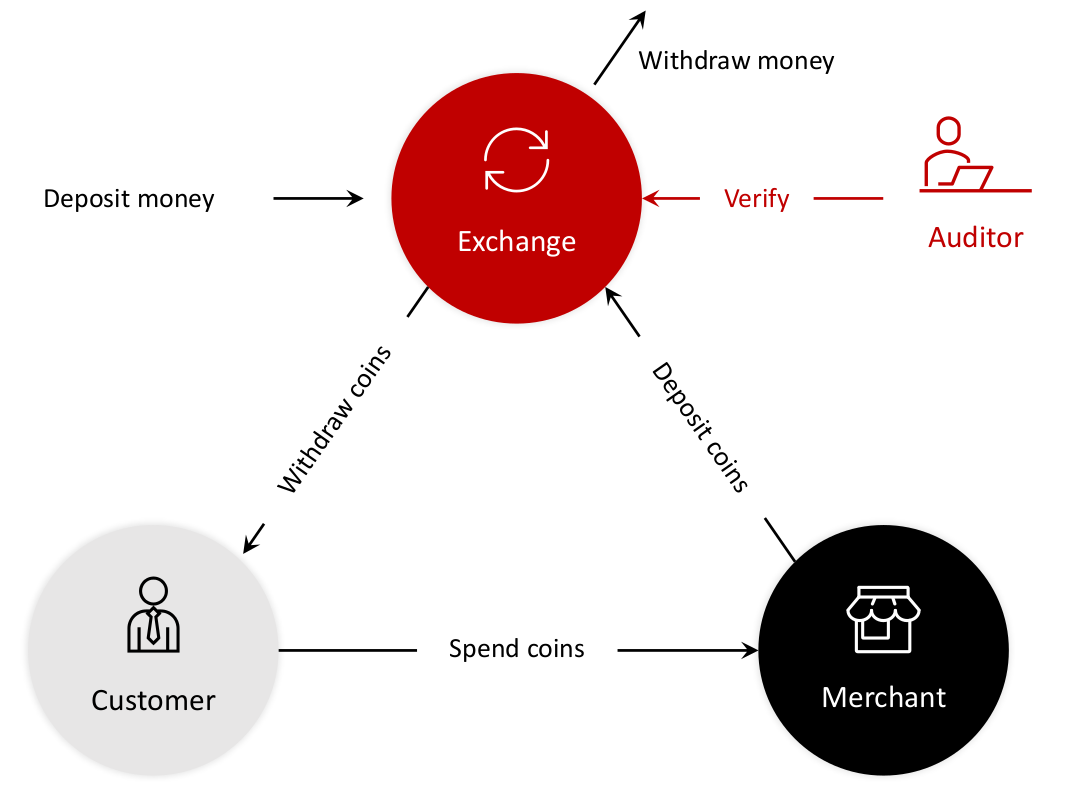
\includegraphics[height=0.6\textwidth]{diagram-simple.png}
    \centering
    \caption{GNU Taler simple overview (source: \cite{pic:simple-diagram})}
    \label{fig:simple-diagram}
\end{figure}

\subsubsection{Exchange}
\label{sec:exchange}
The exchange is the payment service provider for financial transactions between a customer and merchant.
The exchange holds bank money as reserve for the anonymous digital coins.
\\
Details of the exchange's functionality can be found in section 4.3 from Florian Dold's thesis \cite{dold:the-gnu-taler-system} or in the documentation \cite{taler-documentation:exchange-operator-manual}.
\\The code can be found in the exchange's git repository \cite{taler-git:exchange}.

\subsubsection{Customer (Wallet)}
A customer holds Taler Coins in his electronic wallet.
As we see in figure \ref{fig:simple-diagram}, a customer can withdraw coins from the exchange.
These coins can then be spent with a merchant.
\\
Details of the wallet's functionality can be found in section 4.6 from Florian Dold's thesis \cite{dold:the-gnu-taler-system} or in the documentations \cite{taler-documentation:wallet-developer-manual} \cite{taler-documentation:wallet-cli-manual}.
\\
Git Repositories:
\begin{itemize}
    \item Main repository \cite{taler-git:wallet-core} \\
          This Repository includes the wallet-core and the implementations for the web extension and CLI.
    \item Android app \cite{taler-git:android}
    \item iOS app \cite{taler-git:ios}
\end{itemize}

\subsubsection{Merchant}
A merchant accepts Taler Coins in exchange for goods and services.
The merchant deposits these coins at the exchange and receives bank money in return.
\\
Details of the wallet's functionality can be found in section 4.5 from Florian Dold's thesis \cite{dold:the-gnu-taler-system} or in the documentations:
\begin{itemize}
    \item Operator manual \cite{taler-documentation:merchant-backend-operator-manual}
    \item Merchant API \cite{taler-documentation:merchant-api}
    \item Back-Office  \cite{taler-documentation:back-office}
    \item Point-of-Sales \cite{taler-documentation:pos-manual}
\end{itemize}

\noindent Git Repositories:
\begin{itemize}
    \item Backend: \cite{taler-git:merchant}
    \item Backoffice: \cite{taler-git:backoffice}
    \item Point-of-Sales App: \cite{taler-git:android} (part of android repo)
\end{itemize}

\noindent Merchant Frontend Repositories:
\begin{itemize}
    \item Payments with Django: \cite{taler-git:django-payments}
    \item Wordpress woocommerce plugin: \cite{taler-git:woocommerce}
    \item Saleor Frontend: \cite{taler-git:saleor}
    \item Demo Frontends: \cite{taler-git:merchant-demos}
\end{itemize}

\subsubsection{Auditor}
The auditors, which are typically run by financial regulators, have the purpose to monitor the behavior of the exchanges to assure that exchanges operate correctly.
\\
Details of the auditor's functionality can be found in section 4.4 from Florian Dold's thesis \cite{dold:the-gnu-taler-system} or in the documentation \cite{taler-documentation:auditor-operator-manual}.
\\Git Repositories:
\begin{itemize}
    \item Main repository \cite{taler-git:exchange} (Part of exchange repository, inside ./src/auditor and ./src/auditordb)
    \item Auditor's public website \cite{taler-git:auditor}
\end{itemize}

\subsubsection{Bank}
The banks receive wire transfer instructions from customers and exchanges.
As long as the banks can make wire transfers to each other, the Taler parties do not have to have the same bank.

\subsection{Taler Step by Step}
\begin{figure}[htp]
    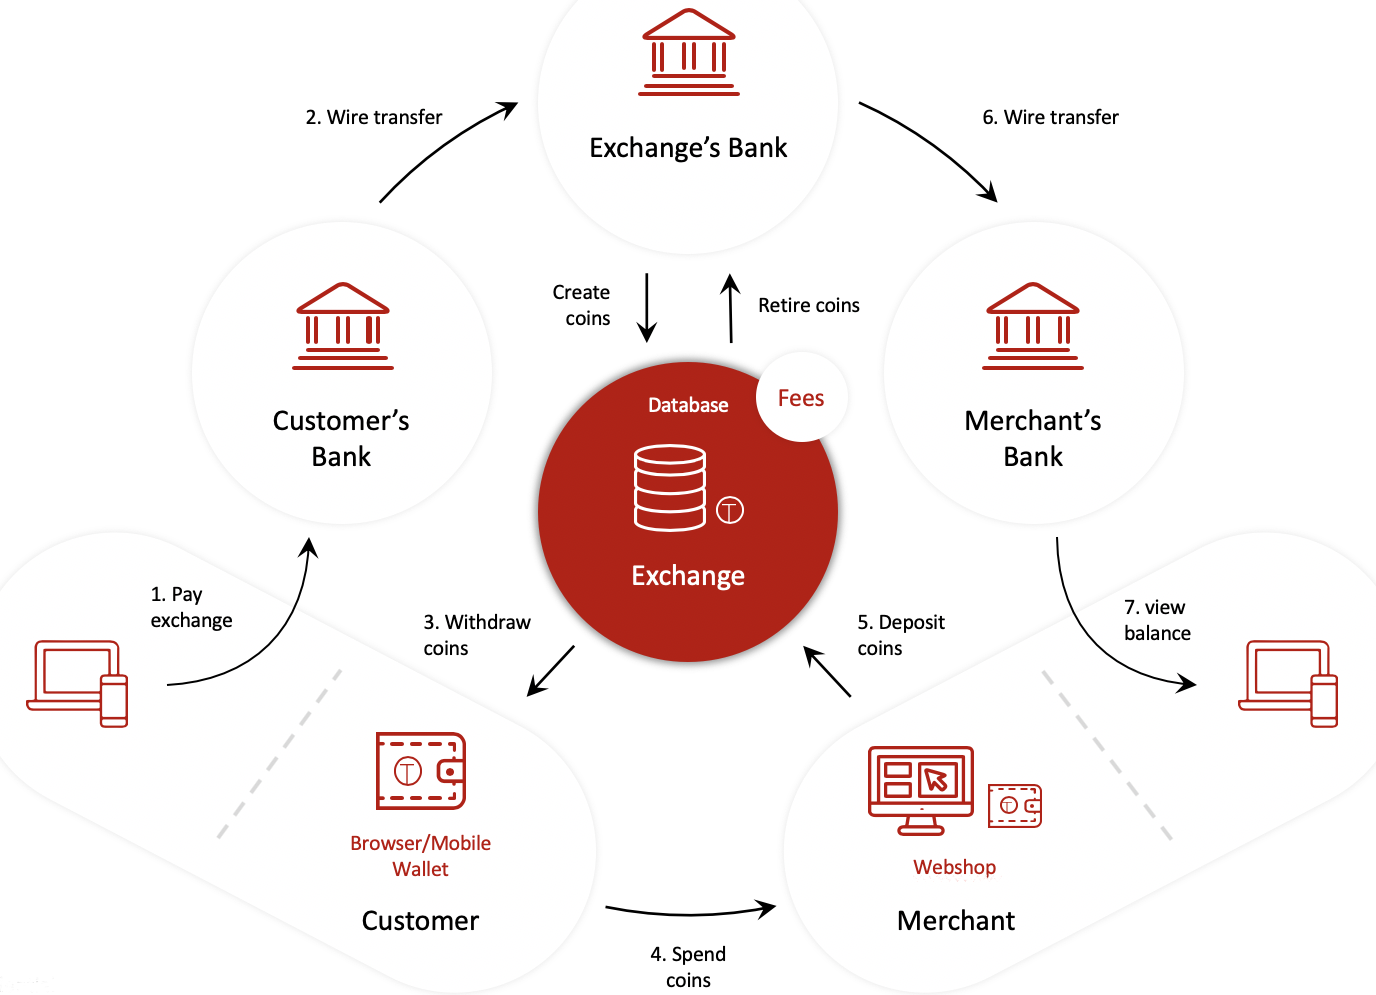
\includegraphics[height=0.65\textwidth]{taler_bigger.png}
    \centering
    \caption{GNU Taler overview (source: \cite{pic:taler-overview})}
    \label{fig:taler-overview-big}
\end{figure}
This is a high-level overview of what Taler generally does.
Many details (like privacy of the buyer, income transparency) are left out and are explained in the following sections.
We see in Figure \ref{fig:taler-overview-big} how Taler works step by step (at a high-level).
\begin{enumerate}
    \item The customer decides to withdraw Taler coins. To do this, he goes to his bank and gives the order to pay the exchange.
    \item The customers bank receives the customers order and makes a wire transfer to the exchanges Bank.
    \item The exchange has received the money and the customer can now withdraw coins to his wallet.
    \item The customer can now spend his coins at a merchant or merchants of his choice.
    \item The merchant can then deposit the coins at the exchange.
    \item The exchanges bank makes a wire transfer to the merchants bank.
    \item The merchant has successfully received the money for the goods he sold.
\end{enumerate}

\subsection{Protocols Overview}
This section provides a high-level overview of the different Taler protocols.
The details are here omitted and discussed later.

\subsubsection{Refresh Protocol}
Taler has a quite interesting protocol to get change.
The purpose of the protocol is to give unlinkable change.
When a customer buys something from a merchant, in most situations he does not have the exact sum in coins.
For this reason, change is needed to provide a convenient payment system.
A coin can be partially spent.
When this happens, the exchange and the merchant know that this coin is used for that specific contract.
If the rest of this coin would be spent in future, one could link these two transactions.
Therefore, a mechanism to get unlinkable change while still preventing money laundering or tax evasion is needed.

\subsubsection{Refund}
Taler has a built-in refund functionality.
Merchants can instruct the exchange to refund a transaction before the refund deadline.
The customer then refreshes the coin(s) in order for payments to remain unlinkable.

\subsubsection{Payment Fees}
The exchange can charge fees for withdrawal, refreshing, deposition of coins.
These fees can depend on the denomination since different denominations can have different storage requirements.
Merchants are able to cover these costs fully or partially.
\\Exchanges are also able to aggregate wire transfers to merchants, thus reducing wire transfer fees.

\subsubsection{Tipping}
Merchants can give customers a small tip.
This feature can be useful for different use cases, for example a merchant can give a tip when a customer participates in a survey.

\subsubsection{Auditing}
Financial auditing is built-in to Taler in the form of auditors.
Auditors have read access to certain exchange databases.
Their task is to verify that exchange work as expected, see chapter 4.4 in Florian Dold's thesis \cite{dold:the-gnu-taler-system} for more details.
In future versions, the auditor will provide an interface that can be used by merchants to submit deposit confirmation samples.
This can be used to detect compromised signing keys or a malicious exchange.

\subsection{Properties}
\label{sec:taler-properties}
%Alle Taler Eigenschaften die wir angreifen wollen auflisten und bezug nehmen wie diese erreicht werden
This section describes Taler's properties.

\subsubsection{Free Software}
The core components of \acl{Taler} are under the following licenses:
\begin{itemize}
    \item exchange \cite{taler-git:exchange}: \ac{GNU AGPL}
    \item merchant \cite{taler-git:merchant}:
          \begin{itemize}
              \item backend: \ac{GNU GPL}v3+, \ac{GNU AGPL}
              \item library: \ac{GNU LGPL}
          \end{itemize}
    \item wallet-core \cite{taler-git:wallet-core}: \ac{GNU GPL}
\end{itemize}

\newpage

\subsubsection{Buyer Privacy Protection}
Taler protects the privacy of buyers during the different stages in the lifetime of a coin:
\begin{enumerate}
    \item Reserve: The reserve is identified by a key pair (private and public key).
          This means that the exchange doesn't know the identity of the reserve account holder.
          Whoever knows the private key is able to withdraw from the corresponding reserve.
    \item Withdrawal: The withdrawal process is encrypted with TLS and uses a blind signature scheme.
          Therefore the exchange doesn't know which customer holds which coin.
    \item Payment: The complete payment process doesn't rely on any information identifying a customer.
\end{enumerate}
Beware that an anonymous bi-directional channel is assumed for communication between the customer and the merchant as well as during the retrieval of denomination key from the exchange and change for partially spent coins (between customer and exchange).

\subsubsection{Merchant Taxability}
Merchant's incomes are transparent to auditors which makes taxation by the state possible.
\newline
A buyer could theoretically transfer the private key and signature of a coin directly to the merchant to bypass the exchange.
However, this is suboptimal for the merchant because the knowledge of the coin doesn't grant him the sole ownership.
If the customer spends the coin in another transaction before the merchant, the coin is voided before the merchant claims its value, thus rendering this form of payment unusable.
The same principle holds for change (refreshed coins) because it is linked to the original coin.
Whoever knows the private key and signature of the original coin can obtain the change and use it before the merchant.

\subsubsection{\acl{AML} and \acl{CFT}}
Every transaction contains the cryptographic hash of the associated contract.
This enables the authorities to request the merchant to reveal the transaction details (the contract).
If the merchant isn't able to reveal the contract, in other words fails to deliver a contract with the same hash which is included in the transaction, he risks punishment or further investigation.
\\Another aspect for \ac{AML} and \ac{CFT} are \ac{KYC} checks.
\acl{KYC} checks require certain institutions to verify certain information about their business partners in order to prevent money laundering and terrorism (see \cite{dewiki:205456999}).
\\\acl{Taler} implements these \ac{KYC} checks:
\begin{itemize}
    \item Exchanges know the identities of their customers.
    \item Merchants might need to pre-register with exchanges (depending on the deployment scenario).
\end{itemize}

\subsubsection{Payer Fraud Prevention}
The following definition was taken from the BigCommerce website \cite{website:bigcommerce-payment-fraud}.
\begin{center}
    \textit{
        "Payment fraud is any type of false or illegal transaction completed by a cybercriminal. The perpetrator deprives the victim of funds, personal property, interest or sensitive information via the internet."
    }
\end{center}
Prevention of payment fraud is a design goal for \acl{Taler}.

\subsubsection{Minimal Information Disclosure}
\acl{Taler} aims to disclose as minimal information as possible.
This mostly concerns customers, but merchants also profit by keeping financial details hidden from competitors.

\subsubsection{\acl{SPOF} Avoidance}
\ac{SPOF}s are fatal because a failure in this component can bring the complete system to a halt.

\subsubsection{Offline Payment (unsupported)}
\acl{Taler} doesn't offer offline payments due to the CAP problem (see chapter "Challenges of offline payments" in \cite{grothoff-dold:euro-bearer-online}).


\section{Cryptographic Preliminaries}
\label{sec:crypto-preliminaries}
In this section we will cover the necessary preliminaries to understand Taler.
For this part we took most of the information from Nigel P. Smarts book Cryptography made simple \cite{modernCrypto} and from the course "Applied Cryptography" at the BFH.
The chapter includes preliminaries of the already implemented cryptographic schemes and the ones that are implemented during this work.

\subsection{Hash Functions}
As source for this section, page 271-275 were used in \textit{Cryptography made Simple}  \cite{modernCrypto}.
\label{sec:hashfunc}
In this paper a hash function is always a cryptographic hash function.
Cryptographic hash function are one-way functions $H()$, which are calculating the hash value $h$ from a message $m$ so that $ h = H(m)$.
With known input one can easily calculate the hash value.
The other way around is computationally infeasible.
\\ Cryptographic hash functions have the following properties.

\subsubsection{(First) Preimage Resistance}
\label{sec:first-pre-resist}
It should be hard to find a message with a given hash value.
For a given output $y$ it is impossible to calculate the input $x$ such that $ h(x) = y$.
\\ This basically means, a hash function can not be inverted, not even with unlimited computing power.
Too much information is destroyed by the hash function and there are many values resulting in the same hash.

\subsubsection{Second Preimage Resistance}
\label{sec:second-pre-resist}
Given one message, it should be hard to find another message with the same hash value.
For a given $x_1$ and $h(x_1)$ it is hard to find a $x_2$ such that $h(x_1) = h(x_2)$.

\subsubsection{Collision Resistance}
\label{sec:col-resist}
It should be hard to find two messages with the same hash value.
It is quite obvious that collisions are existent, since there are more possible messages than hash values.
This is also known as the pigeonhole principle.
Even if there are hash collisions, it should be hard to find $x_1 \ne x_2$ such that $h(x_1) = h(x_2)$.
Due to the birthday paradoxon (a detailed description can be found under \cite{enwiki:1019272750}) it is easier to cause a collision of two arbitrary messages than of a specific message.

\subsection{Key Derivation}
\label{sec:kdf}
A \ac{KDF} derives one or more cryptographically strong secret keys from initial keying material by using a \acl{PRF}.
Therefore, input of a \ac{KDF} is some sort of keying material (e.g. from a key exchange).
Output will be a pseudo-random bit-string, which can be used as new key material.


\subsubsection{\acl{PRF}}
A \ac{PRF} is a deterministic function whose output appears to be random if the input is unknown.
The output is computationally indistinguishable from a true random source.
Different PRFs exist, for example \ac{AES} or HMAC could be used as \ac{PRF}.
In the case of \gls{hkdf}, HMAC is a suitable choice as \ac{PRF}.

\subsubsection{HMAC}
\label{sec:hmac}
A \acl{MAC} (\ac{MAC}) provides \textbf{unforgeability}, which means, only a person who knows the key $k$ can compute the MAC.
Further, a MAC protects the \textbf{message integrity}, since unauthorized changes are being detected.
Last but not least, \textbf{message authenticity} is provided too, since only a person who knows the key can compute the HMAC.
However, it does not provide non-repudation because it is a shared secret.
MACs take a message and a key as input and give the MAC tag as output.
\\One way to design such MACs is by using a hash function.
The obvious way one would design such a function would most likely be: $ t = H(k || m || pad)$
However, this variant would be \textbf{completely insecure} with hash functions based on Merkle-Damgard constructions.
Because of the structure of such hash functions, it is easy to find $H(M || X)$ for an arbitrary $X$ and a hash value $H(M)$, with that a so called \textit{length-extension} attack is possible.
\\HMAC prevents this attack by computing the MAC as follows: $t = $ HMAC$_k(m) = H( (k \oplus opad) || H( (k \oplus ipad) || m) ) $
\\ H() could be any standard hash functions, for example SHA-256, SHA-512 or SHA-3.
$\oplus$ stands for the XOR operation.
HMAC is specified in \cite{rfc2104}.

\subsubsection{HKDF}
\gls{hkdf} follows the \textit{extract-then-expand} paradigm and therefore has two phases.
In the extract phase, the input keying material is taken and a fixed-length pseudorandom key $K$ is \textit{extracted}.
This phase is used to generate a high entropy pseudorandom key from potentially weaker input keying material.
This key $K$ is used in the \textit{expand} phase to output a variable-length, pseudorandom key.

The \gls{hkdf} makes use of HMAC (\ref{sec:hmac}) instantiated with a hashfunction \ref{sec:hashfunc}.
It takes the input keying material, a salt and the length of output keying material as arguments.
\gls{hkdf} is specified in \cite{rfc5869}.

\subsection{Digital Signatures}
\label{sec:sign-schemes}
As source for this section, page 216-218 were used in \textit{Cryptography made Simple}\cite{modernCrypto}.
A digital signature is a cryptographic function used to verify the origin and integrity of a message.
It provides the following properties:
\begin{itemize}
    \item Sender authenticity: The origin/sender of a message can not be forged.
    \item Message integrity: No unauthorized change to the message can be made, the message is tamperproof.
    \item Non-repudiation: After a message is signed, one can not dispute that a message was signed.
\end{itemize}
If verification is successful, only Alice knows her private key and Bob uses Alice's public key to verify, then Bob knows that this message is really from Alice and the message has not been tampered or further modified.
A digital signature scheme has a message space M, a signature space S and three algorithms:
\begin{itemize}
    \item Key generation: $(pk,sk) \gets keyGen()$
    \item Signatue generation: $s \gets $sign$_sk(m)$
    \item Verification: $ v \gets $verify$_pk(m,s)$ where $v \in {0,1}$
\end{itemize}
If the result of the verification algorithm equals 1, a signature for m is called valid.
\\Digital signatures are publicly verifiable, which means anyone can verify that $(m,s)$ is legitimate.

\subsubsection{Adversary Models \& Provable Security}
\label{sec:euf-cma}
Digital Signature schemes are believed to be secure when they are EUF-CMA secure.
\acl{EUF} (\ac{EUF}) means that given a public key $pk$ the adversary cannot construct a message with a valid signature, except with a negligible probability.
\acl{CMA} (\ac{CMA}) means that an adversary can ask a signing oracle to produce valid signatures $s' = sign_{sk}(m')$ for arbitrary messages $m' \ne m$.\\
EUF-CMA is therefore existentially unforgeability under chosen message attack and is a standard security model for digital signatures.
More details can be found in page 217-218 in \textit{Cryptography made Simple} \cite{modernCrypto}.


\subsubsection{RSA-FDH Signature Scheme}
As source for this section, pages 300-301 and 333-335 were used in \textit{Cryptography made Simple} \cite{modernCrypto}.

\label{sec:rsa-fdh}
RSA-FDH is a deterministic digital signature scheme which provides authenticity, message integrity and non-repudation.
The RSA signature scheme (without the full domain hash) is NOT \ac{EUF} secure and is vulnerable to existential forgery attacks.
RSA-FDH is one possible solution for a EUF-CMA secure scheme. EUF-CMA and its adversary model is further discussed in section \ref{sec:euf-cma}.
RSA-FDH is EUF-CMA secure under factoring and RSA assumptions.
More details on the hardness assumptions can be found on page 32-49 in \textit{Cryptography made Simple} \cite{modernCrypto}.

\paragraph{\acl{FDH}}
A \acl{FDH} is a hash function with an \textbf{image size equal to the size of the RSA modulus}.
The hashfunction $h()$ used in the RSA-FDH sign (section \ref{sec:rsa-fdh-sign}) and RSA-FDH verify (section \ref{sec:rsa-fdh-sign}) needs to fulfill all the security properties we defined in chapter \ref{sec:hashfunc}.
This means that the image is a co-domain of the RSA group $\mathbb{Z}_N^*$.
Provided that the hashfunction has properties of a random oracle, \textbf{RSA-FDH is provably EUF-CMA secure} under the RSA assumption.

\paragraph{RSA Key Generation}
\label{sec:rsa-keygen}
The information in this section is from the script of the BFH module \textit{Public Key Cryptography} taught by Prof. Dr. Walter Businger (\cite{businger:public-key-crytpo}).
The RSA private and public key are generated like this:
\begin{enumerate}
    \item Generate two random prime numbers $ p, q $ where $ p \neq q $
    \item Calculate $ N = pq $
    \item Calculate $ \lambda = \text{lcm}(p-1, q-1) $
    \item Randomly choose a number $ d $ which is bigger than $ p $ and $ q $ and where $ \text{gcd}(d, \lambda) = 1 $
    \item Calculate $ e $, the multiplicative inverse of $ d \mod \lambda $
    \item The public key is $ (e, N) $, the private key is $ (d, N) $
    \item Destroy all numbers not included in the private or public key
\end{enumerate}
Note that "lcm" stands for least common multiplier and "gcd" means greatest common divisor.
The original RSA specification uses $ \phi(n) = (p-1)(q-1) $ instead of $ \lambda = \text{lcm}(p-1, q-1) $.
$ \phi(n) $ is a multiple of $ \lambda $ (for details see \cite{businger:public-key-crytpo}).

\paragraph{Signature Algorithm}
\label{sec:rsa-fdh-sign}
The signature can be calculated as following:
\\ $ s \gets (\text{FDH}(m))^d \mod N$

\paragraph{Verification Algorithm}
\label{sec:rsa-fdh-verify}
The signature can be validated as following:
\\ $ \text{FDH}(m) \gets s^e \mod N$

\subsubsection{Schnorr Signature Scheme}
\label{sec:schnorr-sig}
The Schnorr Signature scheme is a randomized signature scheme, which is proven to be EUF-CMA secure under \ac{DLP}.
More information about the \ac{DLP} can be found in chapter 3 of \textit{Cryptography made Simple} \cite{modernCrypto}.
In february 2008 the patent expired and Schnorr signatures are now becoming widely deployed. (eg. EdDSA).
Schnorr signatures gained quite some attraction lately, since Bitcoin has announced to support Schnorr signatures starting from Block 709632 (see \cite{bip:schnorr-bitc}, \cite{btc:releasnotes-0.21}, and \cite{git:secp256k1-schnorr}).
As reference for the Schnorr signature scheme (and later Clause Blind Schnorr Signature Scheme) we use the paper \textit{Blind Schnorr Signatures and Signed ElGamal Encryption in the Algebraic Group Model} \cite{cryptoeprint:2019:877} as general source for Schnorr related schemes.

\paragraph{Setup}
We have a Group $\mathbb{G}$ of order $p$ and a generator $G$ of the group.
Further a Hashfunction $H: \{0,1\}* \rightarrow \mathbb{Z}_p$ is used.

\paragraph{Key Generation}
The key generation is the same as in \ac{DSA}.
\begin{enumerate}
    \item private key is a random integer $x \leftarrow random \in \mathbb{Z}_p$
    \item public key is $X \leftarrow xG$
\end{enumerate}

\paragraph{Sign}
The sign function takes the secret key $x$ and the message $m$ to be signed as argument.
The interactive version with a signer and a user can be seen in figure \ref{fig:schnorr-sign-protocol}.
\begin{enumerate}
    \item choose $r \leftarrow random \in \mathbb{Z}_p $
    \item calculate $R := rG$
    \item $ c := H(R,m)$
    \item $s := r + cx \mod p$
    \item $\sigma := (R,s)$
    \item return $\sigma$
\end{enumerate}

\begin{figure}
    \begin{equation*}
        \begin{array}{ l c l }
            % preliminaries
            \text{User} &  & \text{Signer}
            \\ \text{knows:} & \text{public parameters:} & \text{knows:}
            \\ \text{public key } X & \langle p, \mathbb{G}, G, H\rangle & \text{private signing key } x, X := xG
            \\ & & n \leftarrow random \in \mathbb{Z}_p
            \\ & & R := nG
            \\ & \xleftarrow[\rule{2.5cm}{0pt}]{R} &
            \\ c := H(R,m)
            \\ & \xrightarrow[\rule{2.5cm}{0pt}]{c} &
            \\ & & s := n+cx \mod p
            \\ & \xleftarrow[\rule{2.5cm}{0pt}]{s} &
            \\ \text{check } sG = R + cX
            \\ \sigma := \langle R,s \rangle
        \end{array}
    \end{equation*}
    \caption{Schnorr signature protocol with user who wants to sign a message $m$ by the signer}
    \label{fig:schnorr-sign-protocol}
\end{figure}


\paragraph{Verify}
The verify function takes the public key $X$, the message $m$ and the signature $\sigma$ as argument.
\begin{enumerate}
    \item $ c := H(R,m)$
    \item check $sG = R + cX$
    \item return true if check was successful, false otherwise
\end{enumerate}

The verification holds because $sG = R + cX  $ is $ (r + cx)G = rG + cxG$ which is equal.

\subsubsection{\acl{EdDSA}}
\ac{EdDSA} is a scheme for digital signatures based on twisted Edwards curves and the Schnorr signature scheme.
The information described here originates from \cite{rfc8032} and \cite{enwiki:1013094030}.
\ac{EdDSA} is a general algorithm that can be used with different curves. A choice in curves consists of 11 parameters. These are the most important (the others can be found in \cite{rfc8032}:
\begin{itemize}
    \item odd prime power q (used to generate elliptic curve over finite field $ \mathbb{F}_q $)
    \item integer b, where $ 2^{b-1} > q $, describing the bit size of various elements
    \item cryptographic hash function $ H $ with output size of $ 2b $
    \item base point on curve $ B $ (generator)
    \item number $ c $, (either 2 or 3)
    \item prime number L where $ LB = 0 $ and $2^c*L = \text{number of points on the curve} $
\end{itemize}

\paragraph{Key Creation}
\label{sec:eddsa-keygen}
The private key $ k $ is a random bit-string of length $ b $.
The public key $ A $ is a point on the curve.
To generate it, we calculate $ A = sB $ where $ s = H(k)[:b] $ (meaning that we take the $ b $ least significant bits from the output of the hash function as $ s $).

\paragraph{Signature Creation}
\label{sec:eddsa-signature-creation}
An \ac{EdDSA} signature of a message $ M $ is composed of $ (R, S )$, which are generated as follows:
\begin{align*}
    s & = H(k)[:b]
    \\r &= H(H(k)[b + 1:2b] \text{ || } M )
    \\R &= rB
    \\S &= (r + H(R || A || M) * s) \mod L
\end{align*}
Note that $ [:b] $ means taking the $ b $ least significant bits, $ [b + 1:2b] $ means taking the b most significant bits and $ R || A $ means concatenating $ R $ and $ A $.

\paragraph{Signature Verification}
$ (R, S) $ is the signature, $ M $ is the message, $ A $ is the public key and $c, B $ are curve parameters.
To verify a signature, the following equation must be satisfied:
\\$ 2^cSB = 2^cR + 2^cA*H(R || A || M) $
\\This means that verify() returns 1 if the equation holds and 0 otherwise.

\paragraph{Ed25519}
\label{par:curve25519}
Ed25519 is an \ac{EdDSA} based signature scheme and uses \gls{25519} (see \cite{bern:curve25519}), which offers 128 security bits.
\gls{25519} gets its name from the prime $ 2^{255} - 19 $ and is designed for fast computation and to resist side channel attacks.
\\These are the most important \ac{EdDSA} parameters for Ed25519 (the others can be found in \cite{rfc8032}):
\begin{itemize}
    \item $ q = 2^{255} - 19 $
    \item $ b = 256 $
    \item $ H() $: SHA-512
    \item $ B = (15112221349535400772501151409588531511454012693041857206046113283949847762202, $
          \\ $46316835694926478169428394003475163141307993866256225615783033603165251855960) $
    \item $ c = 3 $
    \item $ L = 2^{252} + 27742317777372353535851937790883648493 $
\end{itemize}
\subsection{Blind Signature Schemes}
\label{sec:blind-sign-schemes}
\label{sec:blind-sign-perfect-blindness}
One could think of blind signatures as a message put into an envelope made of carbon paper. The signer stamps his signature on the envelope and due to the properties of a carbon paper, the message is now signed too. (the stamp "stamps" through the envelope on the message).
The client then can open the envelope, and he possesses a correctly signed message.
This is achieved by the client by blinding the message with a blinding factor before sending to the signer ("blind()" operation).
The signer signs the blinded message and returns the signature of the blinded message to the client.
The client, who possesses the blinding factor can then unblind the signature and gets a signature of the original message ("unblind()" operation).
The explanation above leads us to the additional security property of a blind signature, the \textit{blindness} of signatures.
This property requires that a signer cannot link a message/signature pair to a particular execution of the signing protocol \cite{cryptoeprint:2019:877}.\\
A blind signature scheme is called \textit{perfectly blind} if the generated signature (\textit{unblinded} signature) is statistically independent of the interaction with the signer (\textit{blinded} signature).
Thus, blind signatures cannot be linked to the signer interaction in an information theoretic sense. \cite{schnorr:perfect-dl-signatures} \cite{spring:wallet-db-with-observers}
\subsubsection{RSA Blind Signature Scheme}
\label{sec:blind-rsa-sign}
As source for this section, the course material from "Applied Cryptography" from BFH and \cite{chaum:blind-sign} were used.
The process for receiving a valid signature from the exchange uses a blind signature scheme invented by David Chaum (\cite{chaum:blind-sign}) which is based on RSA signatures.
The process is described in figure \ref{fig:blind-sign}.
\\Note that Bob (the signer) uses a standard RSA signature and can't verify if the message from Alice is blinded.
\begin{figure}[htp]
    \begin{equation*}
        \begin{array}{ l c l }
            \text{Alice} &  & \text{Bob}
            \\ \text{knows:} & & \text{knows:}
            \\ \text{RSA public key } D_B = e, N & & \text{RSA keys } d_B, D_B
            \\ \text{message } m & &
            \\ & &
            \\ \text{blind:} & &
            \\ r \leftarrow random \in \mathbb{Z}_N^* & &
            \\ m' = m*r^{e} \mod N & &
            \\ & \xrightarrow[\rule{2.5cm}{0pt}]{m'} &
            \\ & & \text{sign:}
            \\ & & s' = (m')^{d_B} \mod N
            \\ & \xleftarrow[\rule{2.5cm}{0pt}]{s'} &
            \\ \text{unblind:}& &
            \\ s = s'*r^{-1} & &
        \end{array}
    \end{equation*}
    \caption{Blind signature scheme}
    \label{fig:blind-sign}
\end{figure}
Mathematically a blind signature works similar to the "naive" RSA signature scheme.
We consider Alice as the party who wants to have a message $m$ blindly signed by Bob.
Bob has a public key $D_B = (e, N)$ and his corresponding private key $d_B$ known only by Bob.
Alice needs to generate a random blinding factor $r\in \mathbb{Z}_N^*$, which needs to remain secret.
Alice then calculates $m'=m*r^e \mod N$. The blinded value $m'$ will now be sent to Bob by Alice.
Bob on his side calculates now the signature as usual: $s' = m'^{d_B} \mod N$.
The signature $s' $ is sent to Alice by Bob. Alice can calculate the signature as following: \\$s = s' * r^{-1}$.
\\$s$ is a valid signature of $m$, while the signer, Bob, does not know $m$ nor $b$.
\\We now want to analyze this closer to understand why blind signatures work.
Let's look at this equation:
\\$ s' = m'^{d_B} = (m*r^e)^{d_B} = m^{d_B} * (r^e)^{d_B}$.
\\The interesting part for now is $(r^e)^{d_B}$, since this is $r^1$.
This means the signature $s'$ we got from Bob is $s' = m^{d_B} * r^1$.
Now it is quite obvious how the valid signature $s$ can be calculated by multiplying with the inverse of $r$ as in: $ s =  m^{d_B} * r^1 * r^{-1} = s' * r^{-1}$.

\paragraph{Blindness}
\label{par:prop-blindness-rsa}
\gls{RSABS} are considered \textit{perfectly blind} (see \autoref{sec:blind-rsa-sign}).
There exist multiple $\langle r, m \rangle$ pairs that matches $m'$ such that $m' = m * r^e \mod N$.
Thus, \gls{RSABS} achieves \textit{perfect blindness} which cannot be attacked by brute-force or similar attacks.
Even if a valid $\langle r, m \rangle$ pair is found, the attacker has no possibility to know if it is the correct pair without additional information.

\paragraph{RSA Blinding Attack}
There are also some possible attacks on this scheme.
First this is subject to the RSA blinding attack.
In this attack the property is used, that the signing operation is mathematically equivalent to the encrypt operation in RSA.
The attacker has a ciphertext $c = m^d$ and he wants to break this message.
Now, the attacker uses the ciphertext $c$ as "message" in the blind signature scheme above.
\\$m'' = cr^e \mod n = (m^e \mod n) * r^e \mod n = (mr)^e \mod n$.
    \\The Attacker then sends the blinded message $m''$ to the signer who blindly signs the blinded message.
    \\$s' = m''^d \mod n = (mr)^{ed} \mod n = m*r \mod n$.
\\The attacker recovers the message now with $m = s'*r^{-1} \mod n$.
\\This attack could be prevented by the use of a padding scheme, however this would break RSA symmetry.
In blind signatures the RSA symmetry is needed, otherwise it would produce an incorrect value in the unblind operation.
\\Due to this issue; One should never use the same key for signing and encryption!
A version of blind signatures, RSA-FDH will be discussed, which solves this issue. \cite{enwiki:blind-sign}

\paragraph{Low Encryption Exponent Attack}
For this attack a possibly small message $m$ and a small public key $e$ is given.
If now $c = m^e < n$, one could compute $ m = \sqrt[e]{c} $.
Similar to the RSA blinding attack, padding could solve the issue, however RSA symmetry is needed.
To overcome this issue, RSA-FDH blind signatures are introduced in the next chapter.

\subsubsection{RSA-FDH Blind Signatures}
As source for this section, the course material from "Applied Cryptograhy" from BFH and \cite{chaum:blind-sign} were used.
\label{sec:blind-sign-fdh}
Blind signatures are discussed in \ref{sec:blind-sign-schemes}.
This version is quite similar to the blind signatures already introduced in figure \ref{fig:blind-sign}.
In addition, the \gls{fdh} introduced in section \ref{sec:rsa-fdh} is used.
The difference is that the message does not get directly blinded, it gets hashed before with a \acl{FDH}.
\\Given Alice's message $m$ and Bobs public key $D_B = (e,n)$.
As in the simple \gls{RSABS}, a random blinding factor $r\in \mathbb{Z}_N^*$ is generated.
Before the message is blinded, the \acl{FDH} $ f = \text{FDH}(m)$ is calculated, which then is blinded as in $f' = fr^e \mod n$.
Since the hash function is a \acl{FDH}, $f$ is in the RSA domain $\mathbb{Z}_N^*$.
Now proceed as in the blind signature scheme introduced in the previous section.
The blinded hash $f'$ will be transmitted to Bob who then computes the signature $s' = f'^d \mod n$ and sends $s'$ back.
Alice unblinds $s'$ and gets the valid signature $s = s'r^{-1} \mod n$.

\begin{figure}[htptp]
    \begin{equation*}
        \begin{array}{ l c l }
            \text{Alice} &  & \text{Bob}
            \\ \text{knows:} & & \text{knows:}
            \\ \text{RSA public key } D_B = e, N & & \text{RSA keys } d_B, D_B
            \\ \text{message } m & &
            \\ & &
            \\ Compute f = FDH(m) & &
            \\ & &
            \\ \text{blind:} & &
            \\ r \leftarrow random \in \mathbb{Z}_N^* & &
            \\ f' = f*r^{e} \mod N & &
            \\ & \xrightarrow[\rule{2.5cm}{0pt}]{f'} &
            \\ & & \text{sign:}
            \\ & & s' = (f')^{d_B} \mod N
            \\ & \xleftarrow[\rule{2.5cm}{0pt}]{s'} &
            \\ \text{unblind:}& &
            \\ s = s'*r^{-1} & &
        \end{array}
    \end{equation*}
    \caption{RSA-FDH blind signatues}
    \label{fig:rsa-fdh-blind-sign}
\end{figure}

This version of blind signature is not subject to the attacks introduced in the previous section.

\subsubsection{Blind Schnorr Signature Scheme}
\label{sec:blind-schnorr-sig}
The Blind Schnorr Signature Scheme \textbf{is considered broken} and should not be implemented.
This section is here to explain how blind Schnorr signatures generally work and should help to understand The Clause Blind Schnorr Signature Scheme \ref{sec:clause-blind-schnorr-sig}.

For the signer the calculations are the same as in the original Schnorr Signature Scheme \ref{fig:schnorr-sign-protocol}.
The exchange chooses a random $n \leftarrow random \in \mathbb{Z}_p$ and calculates $R := nG$ as before.
In comparison to the Schnorr Signature Scheme (see section \ref{sec:schnorr-sig}) we generate two random blinding factors $\alpha, \beta \leftarrow random \in \mathbb{Z}_p$ to achieve \textit{blindness}.
The User then calculates $R' := R + \alpha G + \beta X$.
This $R'$ is then used to calculate $c' := H(R',m)$ and is blinded with $b$ as in $c := c' + \beta \mod p$.
The challenge $c$ is then blindly signed by the signer $s := n+cx \mod p$.
The User checks if the signature is valid the same way as in the original protocol.
Finally the user has to unblind $s$ as in $s' := s + \alpha \mod p$.
Now the unblinded signature is $\sigma := \langle R',s' \rangle$.
This scheme is described in figure \ref{fig:schnorr-blind-sign-scheme}.
More details can be found in the \textit{Blind Schnorr Signatures and Signed ElGamal Encryption in the Algebraic Group Model} paper \cite{cryptoeprint:2019:877}.

%The unblinded signature can be verified with $s'G = R' + c'X$, since following equation is satisfied:\\
%$s'G = sG + \alpha G = (r + cx)G + \alpha G = R + \alpha G + \beta X + (-\beta + c)X = R' + c'X = R' + H(R',m)X$ \cite{cryptoeprint:2019:877}.\\

To verify the signature, the verifier has to check if the following equation holds:
\begin{align*}
    s'G & = R' + c' X
    \\ &= R' + H(R', m) X
\end{align*}
$ s', R' $ together form the signature, $ X $ is the public key and $ m $ is message.

The reason why this works is that the original Schnorr signature verification algorithm remains the same in blind signatures.
\begin{align*}
    sG = R + c X
\end{align*}

By replacing $ s, R, c, $ with the values used in the blind signature scheme (as in figure \ref{fig:schnorr-blind-sign-scheme})
\begin{align*}
    \\ s &= s' - \alpha
    \\ R &= R' - \alpha G - \beta X
    \\ c &= c' + \beta
\end{align*}

we receive the following equation:
\begin{align*}
    sG & = R + c X
    \\ (s' - \alpha)G &= R' - \alpha G - \beta X + (c' + \beta)X
    \\ s'G - \alpha G &= R' - \alpha G + c' X
    \\ s'G &= R' + c' X
\end{align*}

\begin{figure}[htp]
    \begin{equation*}
        \begin{array}{ l c l }
            % preliminaries
            \text{User} &  & \text{Signer}
            \\ \text{knows:} & \text{public parameters:} & \text{knows:}
            \\ \text{public key } X & \langle p, \mathbb{G}, G, H\rangle & \text{private signing key } x, X := xG
            \\ & & r \leftarrow random \in \mathbb{Z}_p
            \\ & & R := rG
            \\ & \xleftarrow[\rule{2.5cm}{0pt}]{R} &
            \\ \alpha, \beta \leftarrow random \in \mathbb{Z}_p
            \\ R' := R + \alpha G + \beta X
            \\ c' := H(R',m)
            \\ c := c' + \beta \mod p
            \\ & \xrightarrow[\rule{2.5cm}{0pt}]{c} &
            \\ & & s := r+cx \mod p
            \\ & \xleftarrow[\rule{2.5cm}{0pt}]{s} &
            \\ \text{check } sG = R + cX
            \\ s' := s + \alpha \mod p
            \\ \sigma := \langle R',s' \rangle
        \end{array}
    \end{equation*}
    \caption{The broken Schnorr Blind Signature Scheme}
    \label{fig:schnorr-blind-sign-scheme}
\end{figure}

\paragraph{Blindness}
Blind Schnorr Signatures also achieve \textit{perfect blindness} (\autoref{sec:blind-sign-perfect-blindness}). \cite{spring:wallet-db-with-observers} \cite{cryptoeprint:2019:877}

\paragraph{ROS Problem}
\label{par:ros-problem}
The security of Blind Schnorr Signatures relies on an additional hardness assumption, the \textit{\acl{ROS}} or ROS problem. \cite{Schnorr01securityof}
Solving the \ac{ROS} problem breaks the unforgeability property of blind Schnorr signatures by finding $l + 1$ signatures out of $l$ signing operations.
David Wagner showed in his paper that the \ac{ROS} problem can be reduced to the $(l+1)$-sum problem and therefore showed that an attack is practicable. \cite{wagner:generalized-bday-prob}
More details about \ac{ROS} and Wagner's algorithm can also be found in the paper \textit{Blind Schnorr Signatures and Signed ElGamal Encryption in the Algebraic Group Model} \cite{cryptoeprint:2019:877}.
\\
Due to the possible attack, Blind Schnorr Signatures are considered \textbf{broken} and should not be used.
The next section \ref{sec:clause-blind-schnorr-sig} introduces a modified version for which the \ac{ROS} problem is much harder to solve.
\\
The \ac{ROS} problem is a recent research topic.
Recently a paper about the (in)security of \ac{ROS} was published. \cite{cryptoeprint:2020:945}
The scheme introduced in the next section \ref{sec:clause-blind-schnorr-sig} is considered secure in 2021.
It is important to keep in mind that the \ac{ROS} problem is much newer and there is open research done.

\subsubsection{Clause Blind Schnorr Signature Scheme}
\label{sec:clause-blind-schnorr-sig}
The Clause Blind Schnorr Signature Scheme is a modification of the Blind Schnorr Signature Scheme for which the \ac{ROS} problem is harder to solve.
The Clause Blind Schnorr Signature Scheme does this by choosing two random values $r_0, r_1$ and calculating $R_0 := r_0G; R_1 := r_1G$.
The user generates the blinding factors twice $\alpha_0, \alpha_1, \beta_0, \beta_1 \leftarrow random \in \mathbb{Z}_p$.
The user then calculates the challenges as before $c_0' := H(R_0',m); c_0 := c_0' + \beta_0 \mod p$ and $c_1' := H(R_1',m); c_1 := c_1' + \beta_1 \mod p$.
After the signer receives the two challenges $c_0$ and $c_1$, the signer randomly chooses $b \leftarrow random \{0, 1\}$ and calculates only $s_b$ as in $s := r_b+c_bx \mod p$.
The User receives $s, b$ and can unblind the signature to receive his signature $\sigma := \langle R'_b, s'_b \rangle$.
The verification algorithm remains the same for Clause Blind Schnorr Signature Scheme.
Figure \ref{fig:clause-blind-schnorr-sign-scheme} shows the Clause Blind Schnorr Signature Scheme.
More details about the scheme can be found in the paper \textit{Blind Schnorr Signatures and Signed ElGamal Encryption in the Algebraic Group Model} \cite{cryptoeprint:2019:877}.


\begin{figure}
    \begin{equation*}
        \begin{array}{ l c l }
            % preliminaries
            \text{User} &  & \text{Signer}
            \\ \text{knows:} & \text{public parameters:} & \text{knows:}
            \\ \text{public key } X & \langle p, \mathbb{G}, G, H\rangle & \text{private signing key } x, X := xG
            \\ & & r_0, r_1 \leftarrow random \in \mathbb{Z}_p
            \\ & & R_0 := r_0G
            \\ & & R_1 := r_1G
            \\ & \xleftarrow[\rule{2.5cm}{0pt}]{R_0, R_1} &
            \\ \alpha_0, \alpha_1, \beta_0, \beta_1 \leftarrow random \in \mathbb{Z}_p
            \\ R_0' := R_0 + \alpha_0 G + \beta_0 X
            \\ R_1' := R_1 + \alpha_1 G + \beta_1 X
            \\ c_0' := H(R_0',m)
            \\ c_1' := H(R_1',m)
            \\ c_0 := c_0' + \beta_0 \mod p
            \\ c_1 := c_1' + \beta_1 \mod p
            \\ & \xrightarrow[\rule{2.5cm}{0pt}]{c_0, c_1} &
            \\ & & b \leftarrow random \in \{ 0,1\}
            \\ & & s := r_b+c_bx \mod p
            \\ & \xleftarrow[\rule{2.5cm}{0pt}]{b, s} &
            \\ \text{check } sG = R + cX
            \\ s' := s + \alpha_b \mod p
            \\ \sigma := \langle R_b',s' \rangle
        \end{array}
    \end{equation*}
    \caption{The Clause Schnorr Blind Signature Scheme}
    \label{fig:clause-blind-schnorr-sign-scheme}
\end{figure}

\paragraph{Blindness}
\label{par:prop-blindness-cs}
\gls{CSBS} also achieve \textit{perfect blindness} as in Schnorr Blind Signatures (see \autoref{sec:blind-rsa-sign}). \cite{cryptoeprint:2019:877}


\subsection{Diffie Hellman Key Exchange}
As source for this section, pages 383-386 were used in \textit{Cryptography made Simple} \cite{modernCrypto}.
\label{sec:preliminaries-DHKE}
The \acl{DHKE} is a well proofed and well understood key exchange mechanism.
\ac{DHKE} relies mainly on the \acl{DLP}.
\ac{DHKE} is used for key exchange in many protocols today (e.g. TLS cipher suites).

\subsubsection{Hardness Assumptions}
\label{sec:dlp}
As already stated, the \ac{DHKE} relies on the assumption that calculating the discrete logarithm is hard.
The \ac{DLP} is in $G$, where $G$ is a finite abelian group of prime order q.
This could either be a subgroup of the multiplicative group of a finite field or the set of points on an elliptic curve over a finite field.
Given $g,h \in G$, find x such that $g^x = h$.

Further, \ac{CDH} and \ac{DDH} are important hardness assumption, which can be reduced to the \ac{DLP}.
Hardness assumptions are introduced very briefly.
In this work we believe that these well proofed and well tested hardness assumptions hold.
(See Chapter 3.1 \textit{Cryptography made Simple} \cite{modernCrypto} for more details on DH hardness assumptions.)

\subsubsection{Protocol}
Alice and Bob want to securely exchange a key with \ac{DHKE}.
Alice has a private key $a$ and a corresponding public key $A = g^a \mod p$.
Bob has a private key $b$ and a corresponding public key  $B = g^b \mod p$.
With elliptic curves, the private key is a multiplication factor for a base point $g$ (see example on page 385 \textit{Cryptography made Simple} \cite{modernCrypto}).

Alice now sends her public key $A$ to Bob.
Bob can then calculate $k = A^b \mod p = g^{ab} \mod p$ and sends his public key $B$ to Alice.
Alice can then calculate $k = B^a \mod p = g^{ab} \mod p$.
Both get the same key $k$ as result of the key exchange.
Note: This protocol on its own is not an authenticated key exchange, which means that Man-in-the-Middle attacks are possible.

A different way of looking at \ac{DHKE} is by thinking of a lock which can be unlocked by two (private) keys.
If one of the two private keys are known, one could calculate $k$ on its own.
Taler's refresh protocol (see \ref{sec:refresh-protocol}) uses \ac{DHKE} in a very interesting way.

\subsection{Cut and Choose Protocol}
\label{sec:preliminaries-cut-choose}
A good introduction to cut and choose protocols gives the Paper from Claude Crépeau (\cite{Crépeau2005} References to the important examples can be found in the paper.):
\begin{center}
    \textit{
        "A cut and choose protocol is a two-party protocol in which one party tries to convince another party that some data he sent to the former was honestly constructed according to an agreed upon method.
        Important examples of cut-and-choose protocols are interactive proofs, interactive arguments, zero-knowledge protocols, witness indistinguishable and witness hiding protocols for proving knowledge of a piece of information that is computationally hard to find.
        Such a protocol usually carries a small probability that it is successful despite the fact that the desired property is not satisfied.
        \\\dots\\
        The expression cut-and-choose was later introduced by David Chaum in analogy to a popular cake sharing problem:
        Given a complete cake to be shared among two parties distrusting of each other (for reasons of serious appetite).
        A fair way for them to share the cake is to have one of them cut the cake in two equals hares, and let the other one choose his favourite share.
        This solution guarantes that it is in the formers best interest to cut the shares as evenly as possible."
    }
\end{center}

Talers cut and choose protocol is \textit{zero knowledge}, which means that nothing about the secret is learned.
The cut and choose protocol used in Taler is explained further when the refresh protocol is discussed (see \ref{sec:refresh-protocol}).

\section{Taler Protocols}
In section \ref{sec:taler-intro} a brief overview of how \acl{Taler} works is given. All the relevant preliminaries are covered in section \ref{sec:crypto-preliminaries}.
In this section a closer look at the different protocols is taken.

\subsection{Withdrawal Protocol}
\label{sec:withdrawal}
The withdrawal protocol is described in chapter 4.7.2 of \cite{dold:the-gnu-taler-system}.
Before coins can be withdrawn, the customer generates a reserve key pair $ w_s, W_p \leftarrow Ed25519.KeyGen() $.
He then transfers a certain amount of money from his bank to the exchange's bank via wire transfer.
This payment must include the reserve public key $ W_p $.
The customer will later authorize withdrawals with a signature using his private reserve key.
%The customer can then authenticate, since he is in possession of the private reserve key.
As soon as the exchange has received the payment, the withdrawal for coins with a value $ i $ can begin (described in figure \ref{fig:withdrawal-process}).

At this stage the client knows the reserve private key and the public denomination key.
The customer can then create coins up to the amount included in the wire transfer.
The coin creation and blind signatures are described in section \ref{sec:blind-sign-fdh}.
So the client generates a planchet (an Ed25519 key pair) and blinds it.
This blinded planchet is then signed by the customers private reserve key, to prove that the customer is eligible to withdraw the coin.
The exchange who receives the blinded planchet and the signature first checks whether the signature is valid with the public reserve key sent with the wire transfer.
When successful, the exchange blindly signs the planchet, returns the signature and notes the amount withdrawn of the reserve.
The customer unblinds the signature, checks its validity and persists the coin.
The state machine of a coin can be seen in figure \ref{fig:coin:states}.

\begin{figure}[htp]
    \begin{center}
        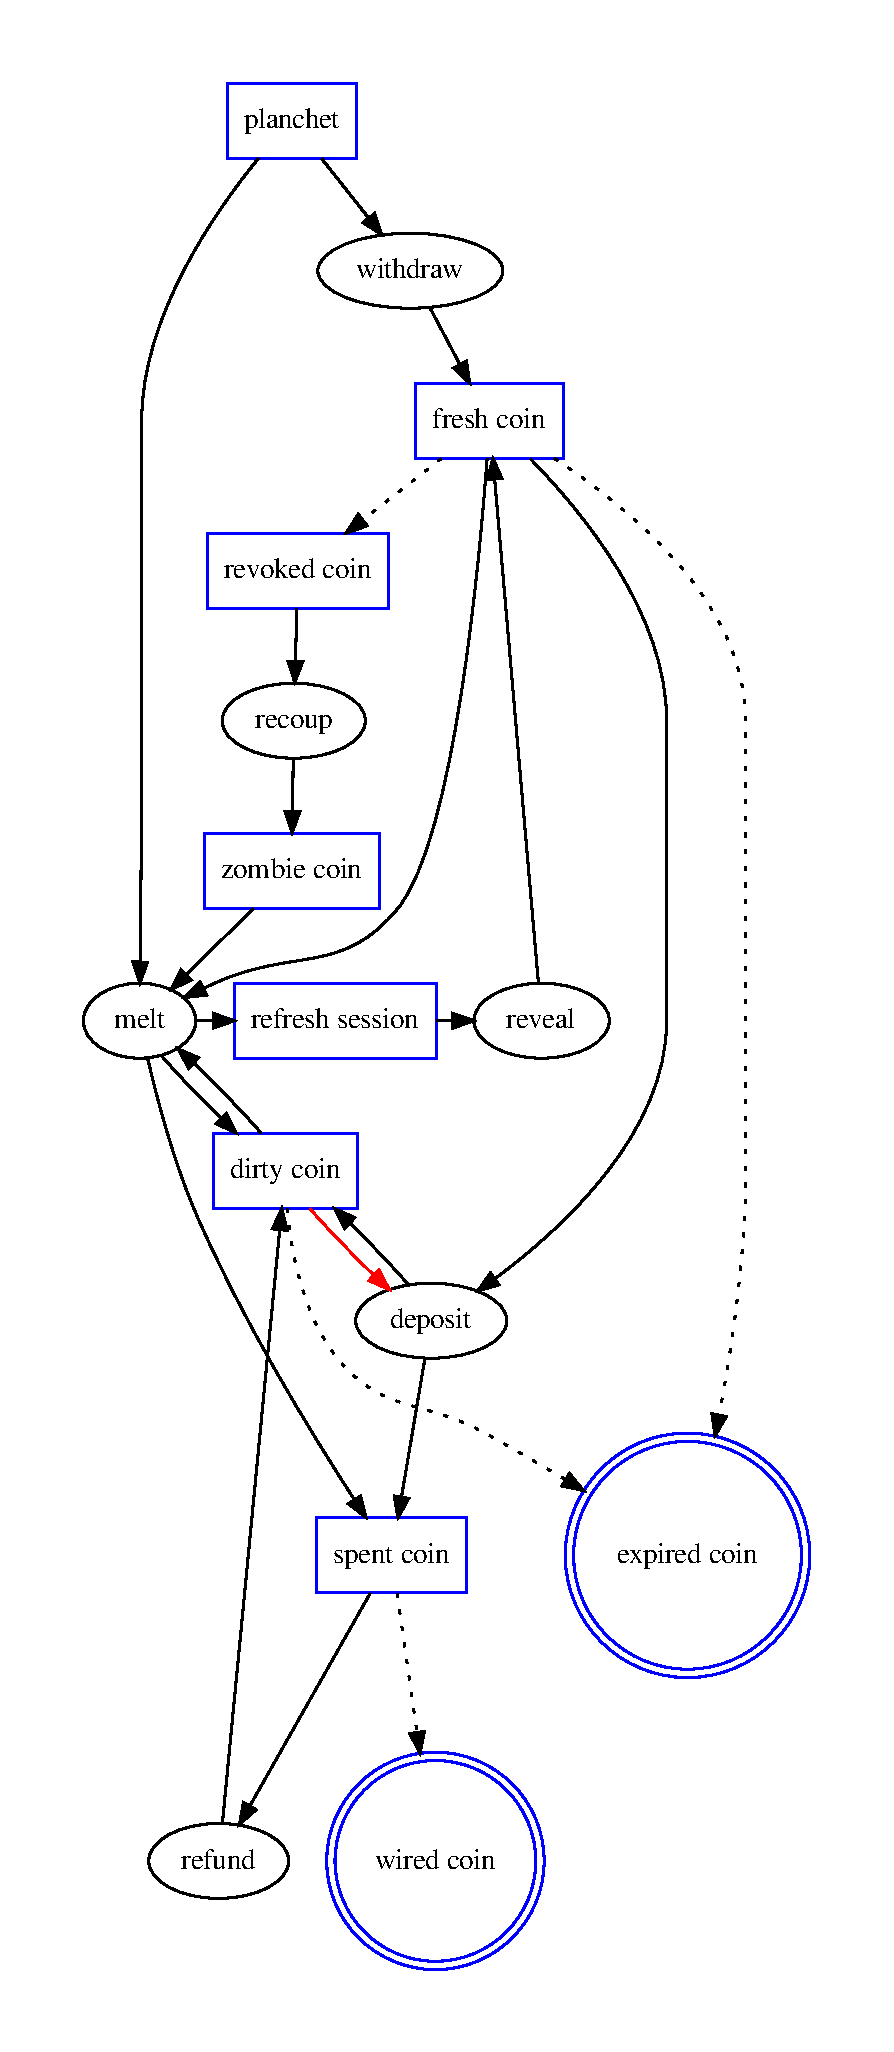
\includegraphics[scale=0.58]{coin.pdf}
    \end{center}
    \caption{State machine of a coin (source: \cite{pic:coin-state-machine})}
    \label{fig:coin:states}
\end{figure}

\begin{figure}[htp]
    \begin{equation*}
        \resizebox{1.0\textwidth}{!}{$\displaystyle
        \begin{array}{ l c l }
            \text{Customer} &  & \text{Exchange}
            \\ \text{knows:} & & \text{knows:}
            \\ \text{reserve keys } w_s, W_p & & \text{reserve public key } W_p
            \\ \text{denomination public key } D_p = e, N & & \text{denomination keys } d_s, D_p
            \\ & &
            \\\text{generate coin key pair:} & &
            \\ c_s, C_p \leftarrow Ed25519.KeyGen() & &
            \\ \text{blind:} & &
            \\ r \leftarrow random \in \mathbb{Z}_N^* & &
            \\ m' = \text{FDH}(N, C_p)*r^{e} \mod N & &
            \\ \text{sign with reserve private key:} & &
            \\ \rho_W = D_p, m' & &
            \\ \sigma_W = \text{Ed25519.Sign}(w_s, \rho_W) & &
            \\ & \xrightarrow[\rule{2.5cm}{0pt}]{\rho = W_p, \sigma_W, \rho_W} &
            \\ & & \text{verify if denomination public key}
            \\ & & \text{is valid}
            \\ & & \text{check } \text{Ed25519.Verify}(W_p, \rho_W, \sigma_W)
            \\ & & \text{decrease balance if sufficient}
            \\ & & \text{sign:}
            \\ & & \sigma'_c = (m')^{d_s} \mod N
            \\ & \xleftarrow[\rule{2.5cm}{0pt}]{\sigma'_c} &
            \\ \text{unblind:}& &
            \\ \sigma_c = \sigma'_c*r^{-1} & &
            \\ \text{verify signature:}& &
            \\ \text{check } \sigma_c^{e} = \text{FDH}(N, C_p) & &
            \\ & &
            \\ \text{resulting coin: } c_s, C_p, \sigma_c, D_p & &
        \end{array}$
        }
    \end{equation*}
    \caption{Withdrawal process}
    \label{fig:withdrawal-process}
\end{figure}

\subsubsection{Withdraw Loophole}
\label{sec:withdraw-loophole}
The withdraw loophole allows withdraw operations where owner of the resulting coins isn't the owner of the reserve that the coins where withdrawn from.
It is used for tipping (described in section \ref{sec:tipping}) and can therefore be seen as a feature.

By misusing the withdraw loophole, untaxed and untraceable payments can be performed.
Figure \ref{fig:withdraw-loophole-exploit} explains how such a payment would work.
Note that we omitted the parts leading up to the coin creation (contract, agreement of price, number of coins and their denominations).
This is how it works on a high level:
\begin{enumerate}
    \item The malicous merchant generates and blinds coins, which are then transmitted to the customer
    \item The customer authorizes the withdraw from his reserve by signing the blinded coins with the private key of his reserve, thus generating withdraw confirmations.
    \item The withdraw confirmations are transmitted to the exchange, which generates the signatures and returns them to the malicous merchant.
    \item The malicous merchant unblinds the signatures.
          He is now in possession of the coin, thus the payment is completed.
\end{enumerate}

\begin{figure}[htp]
    \begin{equation*}
        \resizebox{1.0\textwidth}{!}{$\displaystyle
        \begin{array}{ l c l}
            % preliminaries
            \textbf{Customer}          &  & \textbf{malicous Merchant}
            \\ \text{knows:} & & \text{knows:}
            \\ \text{reserve keys } w_s, W_p
            \\ \text{denomination public key } D_p = \langle e, N \rangle & & \text{denomination public key } D_p = \langle e, N \rangle
            \\
            % generate coin
            \\ & & \text{generate coin key pair:}
            \\ & & c_s, C_p \leftarrow \text{Ed25519.KeyGen}()
            % blind
            \\ & & \text{blind:}
            \\ & & r \leftarrow random \in \mathbb{Z}_N^*
            \\ & & m' := \text{FDH}(N, C_p)*r^{e} \mod N
            % sing with reserve sk
            \\ & \xleftarrow[\rule{2cm}{0pt}]{m'}
            \\ \text{sign with reserve private key:}
            \\ \rho_W := \langle D_p, m' \rangle
            \\ \sigma_W := \text{Ed25519.Sign}(w_s, \rho_W)
            \\ & \xrightarrow[\rule{2cm}{0pt}]{ \langle W_p, \sigma_W, \rho_W \rangle }
            \\
            \hline
            \\
            \textbf{malicous Merchant} &  & \textbf{Exchange}
            \\\text{knows:} & & \text{knows:}
            \\& & \text{reserve public key } W_p
            \\ \text{denomination public key } D_p = \langle e, N \rangle & & \text{denomination keys } d_s, D_p
            \\
            \\ & \xrightarrow[\rule{2cm}{0pt}]{ \langle W_p, \sigma_W, \rho_W \rangle }
            \\ & & \langle D_p, m' \rangle := \rho_W
            \\ & & \text{verify if } D_p \text{ is valid}
            \\ & & \textbf{check } \text{Ed25519.Verify}(W_p, \rho_W, \sigma_W)
            \\ & & \text{decrease balance if sufficient}
            \\ & & \text{sign:}
            \\ & & \sigma'_c := (m')^{d_s} \mod N
            \\ & \xleftarrow[\rule{2cm}{0pt}]{\sigma'_c}
            \\ \text{unblind:}
            \\ \sigma_c := \sigma'_c*r^{-1}
            \\ \text{verify signature:}
            \\ \textbf{check if } \sigma_c = \text{FDH}(N, C_p)
            \\
            \\ \text{resulting coin: } \langle c_s, C_p, \sigma_c, D_p \rangle
        \end{array}$
        }
    \end{equation*}
    \caption{Untaxed payment using the withdraw loophole}
    \label{fig:withdraw-loophole-exploit}
\end{figure}

\subsection{Payment Process}
The payment process is divided in two steps described by the spend and deposit protocols.
Details about the payment process can be found in multiple chapters in \cite{dold:the-gnu-taler-system}:
Chapter 4.7.3 describes the spend and deposit protocols.
Chapter 4.1.4 describes more general aspects as well as the contract header and deposit permission structure and details.
\\On a high level, payment works like this:
\begin{enumerate}
    \item The  customer submits a shopping cart (one or more items to buy) and commits his intent to buy them.
    \item The merchant puts together the contract terms containing the necessary information for payment, signs it and sends both to the customer (spend protocol).
    \item The customer generates a deposit permission and its signature for each coin used in the transaction (spend protocol).
    \item The customer forwards the deposit permission(s) to the merchant (spend protocol).
          If the deposit protocol is performed by the customer, this step can be skipped.
    \item Either the customer or the merchant sends the deposit permission(s) to the exchange (deposit protocol).
    \item The exchange processes the deposit permission and returns a deposition confirmation when successful (deposit protocol).
    \item If the deposit protocol was performed by the customer, the deposit confirmation(s) have to be forwarded to the merchant.
\end{enumerate}

\subsubsection{Spend Protocol}
The payment process begins when a customer submits a shopping cart (one or more items to buy) and commits his intent to buy them.
The merchant has a key pair skM, pkM of which the customer knows the public key.
% besseres Wort als commit?
Note that certain details contained in contract header or deposit permission like merchant \ac{KYC} information, deposit and refund deadlines and fees are left out.
The deposit state machine can be seen in figure \ref{fig:deposit:states}.
\begin{figure}[htp]
    \begin{center}
        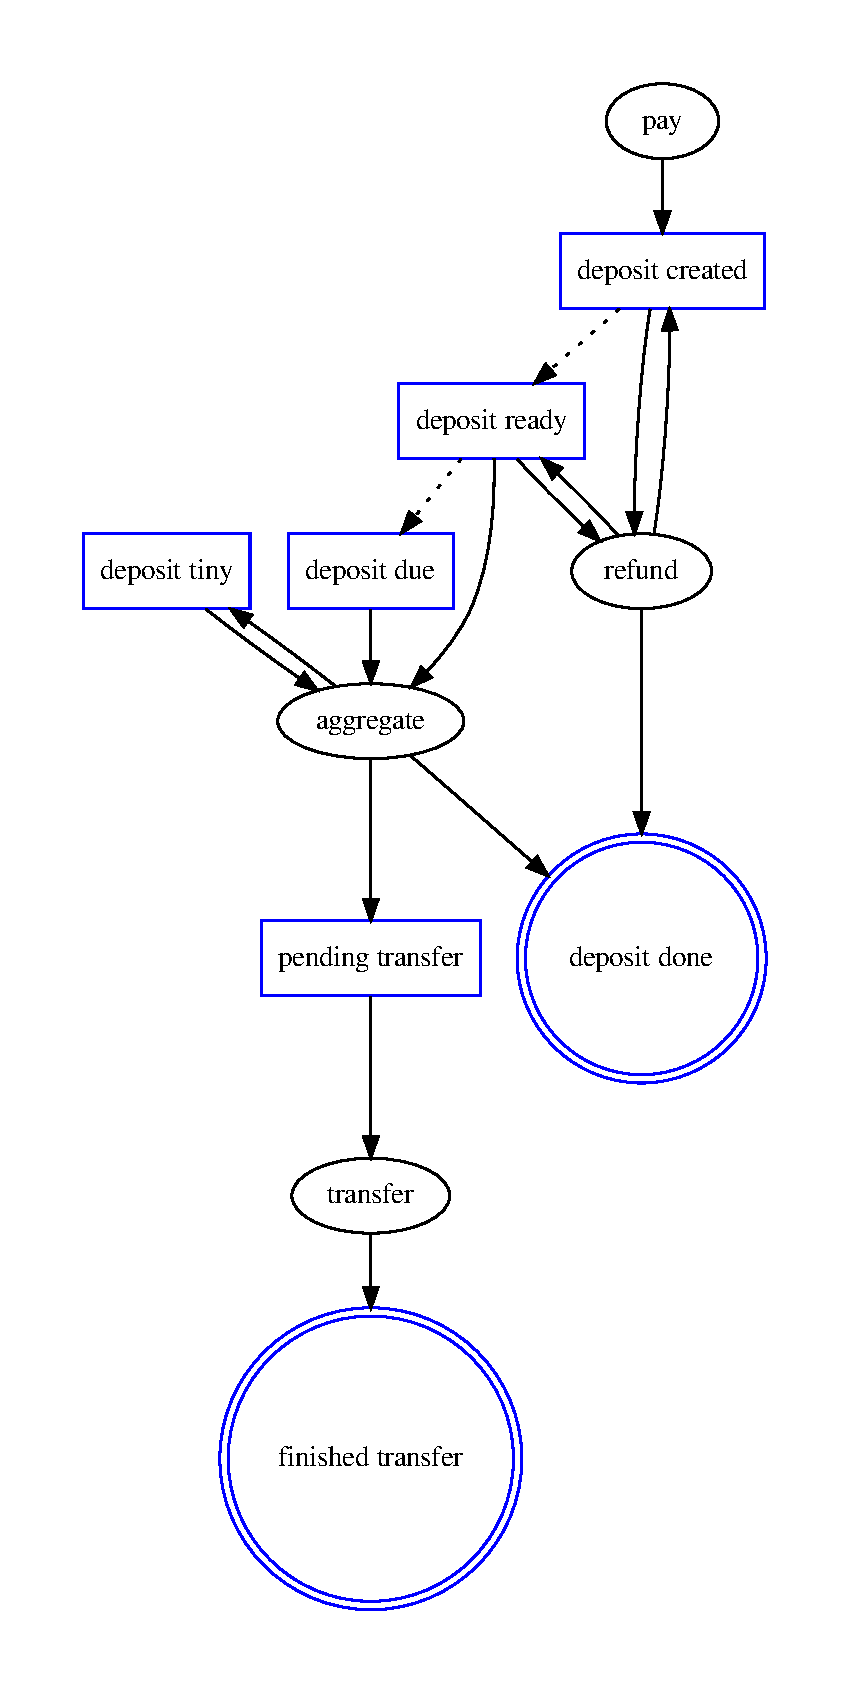
\includegraphics[scale=0.7]{deposit.pdf}
    \end{center}
    \caption{State machine of a deposit (source: \cite{pic:deposit-state-machine})}
    \label{fig:deposit:states}
\end{figure}

\begin{enumerate}
    \item The merchant puts together the following information (without transmitting them) and requests payment:
          \begin{itemize}
              \item price $ v $
              \item exchange $E_m$ (multiple possible)
              \item account $A_m$ at the exchange $E_m$
              \item info (free form details containing the full contract)
          \end{itemize}
    \item The customer generates an Ed25519 claim key pair $ p_s, P_p $ and submits the public key to the merchant.
          This key can be used by the customer to prove that he didn't copy contract terms from another customer.
    \item The merchant puts together the contract terms $ \rho  $ and signs it with skM, resulting in the signature $ \sigma_P$.
          \\The contract terms contains:
          \begin{itemize}
              \item $E_m$ (exchange)
              \item $A_m$ (account at exchange $E_m$)
              \item pkM
              \item Hash($v$, info)
              \item $ P_p $
          \end{itemize}
          $ \rho_P $ (contract terms), $ \sigma_P$ (contract terms signature), $ v $ (price) and info are submitted to the customer.
    \item The customer does the following checks:
          \begin{itemize}
              \item Is the signature of the contract terms correct?
              \item Is the public key referenced in the contract terms the same as the one generated in step 2?
              \item Is the hash of price and info the same as the one in the contract terms?
          \end{itemize}
          If all checks are successful, the customer chooses one or more coins to be spent.
          For each coin, a deposit permission $ \rho_{D} $ and its signature $ \sigma_{D} $ is generated.
          The deposit permission contains the following information:
          \begin{itemize}
              \item Coin public key $ C_p $
              \item Coin denomination public key pkD
              \item Coin signature $ \sigma_C $
              \item Value to be spent for this coin $f$ (greater than zero, up to the residual value of the coin)
              \item Hash of the contract terms $ \rho_P $
              \item Account of merchant $A_m$ (at exchange $E_m$)
              \item Merchant public key pkM
          \end{itemize}
          The list of deposit permissions and their signatures is transferred to the merchant who then executed the deposit protocol.
          Note that the customer is also able to deposit the coins (instead of the merchant), this is used in cases where the merchant doesn't have an internet connection, but the customer does.
          This can be useful in cases where the merchant becomes unresponsive.
          The customer can prove that he paid in time.
    \item The merchant receives the deposit permissions and signatures and uses the deposit protocol to execute the payment.
\end{enumerate}

Before we continue with the deposit protocol, there are a few interesting details to point out (described in \cite{dold:the-gnu-taler-system} section 4.1.4):
\begin{itemize}
    \item The contract terms and the deposit permission are \ac{JSON} objects.
    \item The contract terms only contains a cryptographic hash of the contract.
          This improves privacy since the exchange doesn't have to know the full contract details, but still makes it possible to identify the contract in case of a dispute or some form of auditing.
    \item At the point where the merchant completes step three (submits the contract terms and its signature) to the customer, the customer is able to finish the transaction using the deposit protocol without interaction of the merchant.
          This means that the merchant at this step must be able to fulfill the contract if the customer completes the payment process.
\end{itemize}

\subsubsection{Deposit Protocol}
\label{sec:deposit-protocol}
As previously mentioned, both parties (customer and merchant) are able to run the deposit protocol.
In the following description, the term merchant will be used, but could be replaced by customer.
In cases where there are multiple deposit permissions (meaning that multiple coins are used to pay), the deposit protocol is run separately for each deposit permission.
\begin{enumerate}
    \item The merchant submits the deposit permission and its signature to the exchange.
    \item The exchange runs these checks:
          \begin{itemize}
              \item Is the denomination public key referenced in the deposit permission valid (issued by the exchange, lifetime between start and deposit/refresh expiration, not revoked)?
              \item Is the deposit permission signature $ \sigma_{D} $ a correct signature of the deposit permission $ \rho_{D} $ with the Ed25519 coin public key $ C_p $ referenced in the deposit permission?
              \item Is there a processed deposit recorded in the exchanges databases based on coin public key and contract terms hash (replay/double spending)?
                    If not, continue with the next check since this is correct and expected behavior.
                    \\If there is, does the recorded deposit permission equal the one we're currently checking?
                    If this is the case, further checks can be skipped and the deposit confirmation signature can be returned to the customer.
                    If not, the process should be terminated because there's something wrong with the transaction.
              \item Is the signature of the coin valid?
              \item Is $ f $ (the value to be spent) smaller or equal the residual value of the coin (check for overspending attempt)?
          \end{itemize}
          If all checks are successful, the exchange saves the deposit record containing the deposit permission and its signature in a database, substracts the spent value from the residual value of the coin and schedules the money transfer to the merchant's account $ A_m $ (grouping payments is done to reduce payment fees).
          \\The exchange calculates a deposit confirmation signature $ \sigma_{DC} $ for the deposit permission with the exchange signing private key and returns them to the merchant.
          \\This signature is also used to prove that a merchant was the first to receive payment from a certain coin.
          Without this, an evil exchange could later deny confirming a payment and claim double spending.
          With the signature, the merchant can prove that the payment was confirmed by the exchange, thus delegating the responsibility (and potential financial loss) for double spending detection to the exchange.
    \item The merchant checks the signatures of the deposit confirmations with the exchange signing public key.
\end{enumerate}

It may happen that a payment gets stuck as partially complete, for example when a backup of a wallet is restored and one coin or more have already been spent (\cite{dold:the-gnu-taler-system} chapter 4.1.4).
In this case, the customer can retry the payment with a different coin.
If this isn't possible, the payment can be refunded (assuming refunds were enabled for this payment).
Other scenarios were described in Dold's thesis, but dismissed due to privacy concerns.
This means that disputes have to be settled aside from Taler when a customer isn't able to fully pay and refunds are disabled.

\subsubsection{Web Payment Scenarios}
The following methods are Taler-native methods for paying and payment validation.
They are not identity-based, meaning that they do not require a login or similar techniques.
Note that other methods could be implemented depending on the scenario.

\begin{itemize}
    \item \textbf{Resource-based web payment} (\cite{dold:the-gnu-taler-system} chapter 4.1.5):
          All Taler contract terms contain a fulfillment URL.
          This can either be a direct link to a digital product (like a movie, a song or a document), or to a confirmation page.
          When a browser opens a fulfillment URL for a resource that hasn't yet been paid for, the merchant requests payment.
          The wallet then generates and submits a claim key pair, thus claiming the contract, which then can be paid (if the user accepts the contract).
          The browser can then retry to navigate to the fulfillment URL, this time submitting the contract order ID as parameter, which the merchant can check if it has been paid (and deliver the content if this is the case).
          This is known as the extended fulfillment URL
          \\The wallet stores fulfillment URLs and their associated contracts.
          Upon receiving a payment request, the wallet searches the stored fulfillment URLs and if it found one, automatically forwards the user to the extended fulfillment URL containing the contract.
    \item \textbf{Session-bound payments and sharing} (\cite{dold:the-gnu-taler-system} chapter 4.1.6):
          So far, validating payment is done using the extended fulfillment URL.
          The problem with this approach is that this URL can be shared, which is a problem for digital content.
          To make this more difficult, the seller's website assigns the user a session ID (for example using a session cookie) and extends the extended fulfillment URL with a session signature parameter.
          This parameter can be used by the merchant to check if the user paid for the resource or replayed the payment in this session.
    \item \textbf{Embedded content} (\cite{dold:the-gnu-taler-system} chapter 4.1.7):
          When paying to access multiple resources behind a paywall (instead of just one resource), the previously described methods do not work.
          Dold's thesis suggest two methods:
          \begin{enumerate}
              \item A session cookie can be set by accessing the fulfillment URL.
                    When the browser requests a subresource, the merchant can verify the session cookie.
              \item In this scenario, the fulfillment URL would show the resources behind the paywall.
                    Upon opening the extended fulfillment URL, the merchant's website would add an authentication token to the URLs of the subresources.
                    When accessing a subresource, the merchant can check the authentication tokens validity.
          \end{enumerate}
\end{itemize}

\subsection{Refresh Protocol}
\label{sec:refresh-protocol}
This section provides a description of the refresh protocol.
The technical details can be found in 4.7.4 \cite{dold:the-gnu-taler-system}.
All relevant preliminaries needed to understand the technical details were already introduced in this work.

\subsubsection{Introduction}
A protocol to refresh coins is needed for many reasons.
One important reason is giving change.
Similar to the real world, there are often situations where one does not have the exact amount of coins.
A change protocol therefore provides a lot of convenience for the users.
Without such a mechanism it would be quite hard to use. \\
Giving change is not trivial, since \ac{AML} and \ac{CFT} compliance still needs to hold.
On the other side, the change still needs to provide privacy for the customer.
Thus, the change must be unlinkable to the previous (or any) transaction.\\
Complying with \ac{AML} and \ac{CFT} while preserving the customer's anonymity may sound like a contradiction at first.
However, Taler has a clever way to solve this problem with the refresh protocol.

The general idea is that the new coin can be derived from the private key of the old coin.

\subsubsection{DH Lock}
\ac{DHKE} was introduced in section \ref{sec:preliminaries-DHKE}.
Taler uses \ac{ECDH} as a lock with two possible keys to unlock the shared key.
To create such a lock, one creates two key pairs $C = cG$ and $T = tG$.
To unlock now means calculating $k$.
Both private keys, $c$ and $t$ are now able to calculate $k = tC = t(cG) = c(tG) = cT$ and thus can unlock the lock.
This $k$ can then be used to derive the private key of the new coin and the corresponding blinding factor.

\subsubsection{Customer Setup}

The customer, which holds the old partially spend coin and knows \\$C_{old} = \text{Ed25519.GetPub}(c_{old})$.
    A transfer key $T = \text{Ed25519.GetPub}(t)$ is then (randomly) generated by the customer.
    \\The key pairs $T = \text{Ed25519.GetPub}(t)$ and $C_{old} = \text{Ed25519.GetPub}(c_{old})$ form the lock with two keys that was introduced before.
    The customer then creates $x = c_{old}, T = tC_{old}$ and derives $c_{new}$, the private key of the new coin and $b_{new}$ the blinding factor of the new key.
    As usual the customer calculates the coins public key $C_{new} = \text{Ed25519.GetPub}(c_{new})$, hashes the new coin with \gls{fdh} $f_{new} = \text{FDH}(C_{new})$ and blinds the hash $f'_{new} = f_{new}b_{new}^e$.
    The $f'_{new}$ is then transmitted to the exchange.
    \\Figure \ref{fig:refresh-derive} shows how the new coin is derived as explained above.

    \begin{figure}[htp]
        \centering
        \fbox{%
            \procedure[codesize=\small]{$\text{RefreshDerive}(s, \langle e,N\rangle, C_p)$}{%
                t := \text{HKDF}(256, s, \text{"t"}) \\
                T := \text{Curve25519.GetPub}(t) \\
                x := \textrm{ECDH-EC}(t, C_p)  \\
                r := \text{SelectSeeded}(x,\mathbb{Z}^*_N)\\
                c'_s := \text{HKDF}(256,x,"c")\\
                C'_p := \text{Ed25519.GetPub}(c'_s)\\
                \overline{m} := r^e * C'_p \mod N\\
                \pcreturn \langle t, T, x, c_s', C_p', \overline{m}\rangle
            }
        }
        \caption[RefreshDerive algorithm]{The RefreshDerive derives a new coin from a dirty coin with a seed. The DH-Lock is used to create the link used in the linking protocol}
        \label{fig:refresh-derive}
    \end{figure}

    Now with the DH Lock the person who is in possession of the old key can always recalculate and thus spend the new coin (as long as it knows the public transfer key $T$).
    However, there is one last thing: How does the exchange know that the old key is linked to the new one?
    To comply with \ac{AML} and \ac{CFT}, the exchange wants to ensure that the person who created the new coin is also in possession of the old coin.
    A link needs to be created in a way that nobody can link the old coin to the new coin, except the person in possession of the old coin.
    The person in possession of the old coin needs to proof to the exchange that this link was created without revealing the link.
    This problem is solved with the cut and choose protocol in the next section.

    \begin{figure}[htp]
        \centering
        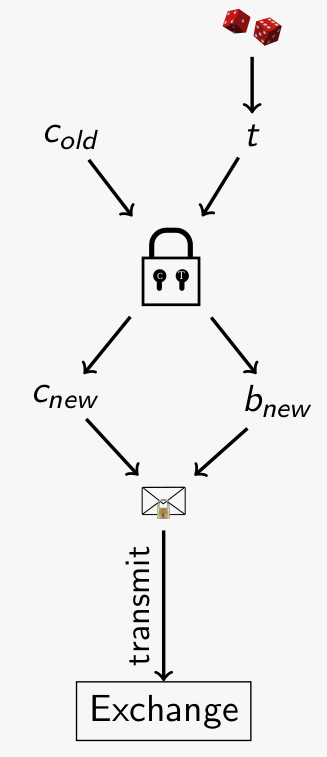
\includegraphics[height=0.5\textwidth]{taler_refresh_transfer_key.png}
        \caption{Taler refresh protocol, transfer key setup (source: \cite{pic:refresh-prot})}
        \label{fig:taler-refresh-transfer-key}
    \end{figure}
    \newpage
    \subsubsection{Cut \& Choose}
    Instead of doing the customer setup once, it is done $n$ times.
    The customer generates $n$ different transfer keys $t_1, t_2 \dots t_n$.
    For each key the whole calculations are done and all the blinded coins $f'_1, f'_2 \dots f'_n$ are sent to the exchange together with the old coins public key and signature. \\
    The exchange responds with a randomly picked number from $1$ to $n$.
    The customer has to reveal all the transfer keys, \textbf{except the one picked by the exchange.}
    The exchange makes the same calculations with the revealed private transfer keys (without knowing the private key $c_{old}$).
    The exchange can now verify whether the customer was honest or not.
    A evil customer could create a new coin which is not linked to the old coin (without the DH lock).
    Such attacks will be detected with a high probability in this protocol.
    Since the $t_x$ picked by the exchange is not checked, an evil customer can win this with a probability of $1/n$.
    Already with $n=3$ an attack is not in the customers interest due to economic reasons.
    In 2 out of 3 cases the exchange would detect the attack and would keep the money and the customer would have lost it.
    The probability can be adjusted with $n$.
    With increasing size of $n$ the attack becomes even less attractive.
    When the cut and choose protocol ended successfully, the value of the old coin is set to zero.

    \begin{figure}[htp]
        \centering
        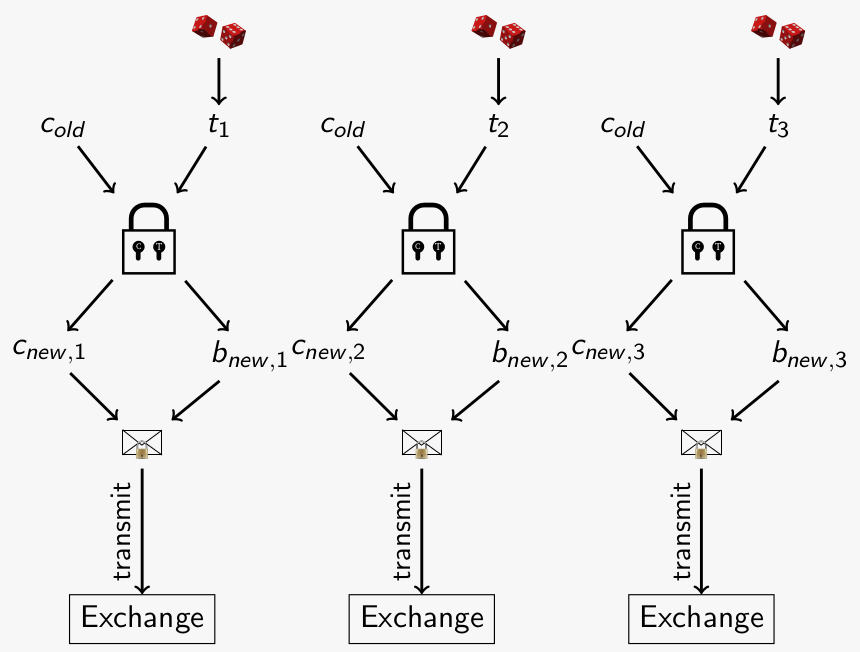
\includegraphics[height=0.5\textwidth]{taler_cut_and_choose.png}
        \caption{Taler refresh protocol, cut and choose (source: \cite{pic:refresh-prot})}
        \label{fig:taler-cut-and-choose}
    \end{figure}

    \subsection{Commit Phase}
    \label{sec:commit-phase-rsa}
    The refresh protocol is implemented in two phases.
    The commit phases creates $k$ derives and commits to this values by calculating a hash over the derives.
    On the exchange's side various checks are done to validate the request.
    Detailed steps of the commit phase are shown in figure  \ref{fig:refresh-part1}.

    
    \begin{figure}
        \begin{equation*}
        \resizebox{1.0\textwidth}{!}{$\displaystyle
            \begin{array}{ l c l }
                % preliminaries
                \text{Customer} &  & \text{Exchange}
                \\ \text{knows:} & & \text{knows:}
                \\ \text{denomination public key } D_{p(i)} & & \text{denomination keys } d_{s(i)}, D_{p(i)}
                \\ \text{coin}_0 = \langle D_{p(0)}, c_s^{(0)}, C_p^{(0)}, \sigma_c^{(0)} \rangle & &
                % refresh request
                \\ \text{Select} \langle N_t, e_t\rangle := D_{p(t)} \in D_{p(i)}
                \\ \textbf{for } i = 1, \dots, \kappa: % generate k derives
                \\ s_i \rightarrow \{0,1\}^{256} % seed generation
                \\ X_i := \text{RefreshDerive}(s_i, D_{p(t)}, C_p^{(0)})
                \\ (t_i, T_i, x_i, c_s^{(i)}, C_p^{(i)}, \overline{m}_i) := X_i
                \\ \textbf{endfor}
                \\ h_T := H(T_1, \dots, T_k)
                \\ h_{\overline{m}} := H(\overline{m}_1, \dots, \overline{m}_k)
                \\ h_C := H(h_t, h_{\overline{m}})
                \\ \rho_{RC} := \langle h_C, D_{p(t)}, D_{p(0)}, C_p^{(0)}, \sigma_C^{(0)}  \rangle
                \\ \sigma_{RC} := \text{Ed25519.Sign}(c_s^{(0), \rho_{RC}})
                \\ \text{Persist refresh-request} \langle \rho_{RC}, \sigma_{RC} \rangle
                \\ & \xrightarrow[\rule{2.5cm}{0pt}]{\rho_{RC}, \sigma_{RC}} &
                % Exchange checks refresh request
                \\ & & (h_C, D_{p(t)}, D_{p(0)}, C_p^{(0)}, \sigma_C^{(0)} = \rho_{RC})
                \\ & & \textbf{check} \text{Ed25519.Verify}(C_p^{(0)}, \sigma_{RC}, \rho_{RC})
                \\ & & x \rightarrow \text{GetOldRefresh}(\rho_{RC})
                \\ & & \textbf{Comment: }\text{GetOldRefresh} \\(\rho_{RC} \mapsto \{\bot,\gamma\})
                \\ & & \pcif x = \bot
                \\ & & v := D(D_{p(t)})
                \\ & & \langle e_0, N_0 \rangle := D_{p(0)}
                \\ & & \textbf{check } \text{IsOverspending}(C_p^{(0)}, D_ {p(0)}, v)
                \\ & & \textbf{check } D_{p(t)} \in \{D_{p(i)}\}
                \\ & & \textbf{check } \text{FDH}(N_0, C_p^{(0)}) \equiv_{N_0} (\sigma_0^{(0)})^{e_0}
                \\ & & \text{MarkFractionalSpend}(C_p^{(0)}, v)
                \\ & & \gamma \leftarrow \{1, \dots, \kappa\}
                \\ & & \text{Persist refresh-record } \langle \rho_{RC},\gamma \rangle
                \\ & & \pcelse
                \\ & & \gamma := x
                \\ & & \textbf{endif}
                \\ & \xleftarrow[\rule{2.5cm}{0pt}]{\gamma} &
                \\
                \\
                \\ & \textit{Continued in figure \ref{fig:refresh-part2}} &
                %\\ \pcintertext[dotted]{(Continued in Figure)}
            \end{array}$
            }
        \end{equation*}
        \caption{Refresh protocol (commit phase)}
        \label{fig:refresh-part1}
    \end{figure}

    \subsection{Reveal Phase}
    \label{sec:reveal-phase-rsa}
    In the reveal phase the customer receives $\gamma$ and he reveals the all the seeds to the exchange, except for $s_\gamma$.
    The exchange can then verify if the customer was honest with probability $1/k$.
    On success the exchange will return the blinded signature of the new coin and the customer can then unblind and store the coin.
    The reveal phase is described in figure \ref{fig:refresh-part2}

    \begin{figure}
        \begin{equation*}
            \resizebox{1.0\textwidth}{!}{$\displaystyle
            \begin{array}{ l c l }
                % preliminaries
                \text{Customer} &  & \text{Exchange}
                \\ & \textit{Continuation of figure \ref{fig:refresh-part1}} &
                \\
                \\
                % Check challenge and send challenge response (reveal not selected msgs)
                \\ & \xleftarrow[\rule{2.5cm}{0pt}]{\gamma} &
                \\ \textbf{check } \text{IsConsistentChallenge}(\rho_{RC}, \gamma)
                \\ \textbf{Comment: } \text{IsConsistentChallenge}\\(\rho_{RC}, \gamma) \mapsto \{ \bot,\top \}
                \\
                \\ \text{Persist refresh-challenge} \langle \rho_{RC}, \gamma \rangle
                \\ S := \langle s_1, \dots, s_{\gamma-1}, s_{\gamma+1}, \dots,s_x \rangle % all seeds without the gamma seed
                \\ \rho_L = \langle C_p^{(0)}, D_{p(t)}, T_{\gamma},\overline{m}_\gamma \rangle
                \\ \rho_{RR} = \langle T_\gamma, \overline{m}_\gamma, S \rangle
                \\ \sigma_{L} = \text{Ed25519.Sign}(c_s^{(0)}, \rho_{L})
                \\ & \xrightarrow[\rule{2.5cm}{0pt}]{\rho_{RR},\rho_L, \sigma_{L}} &
                % check revealed msgs and sign coin
                \\ & & \langle T'_\gamma, \overline{m}'_\gamma, S \rangle := \rho_{RR}
                \\ & & \langle s_1,\dots,s_{\gamma-1},s_{\gamma+1},\dots,s_\kappa \rangle ) := S
                \\ & & \textbf{check } \text{Ed25519.Verify}(C_p^{(0)}, \sigma_L, \rho_L)
                \\ & & \pcfor i = 1,\dots, \gamma-1, \gamma+1,\dots, \kappa
                \\ & & X_i := \text{RefreshDerive}(s_i, D_{p(t)}, C_p^{(0)})
                \\ & & \langle t_i, T_i, x_i, c_s^{(i)}, C_p^{(i)}, \overline{m}_i \rangle := X_i
                \\ & & \textbf{endfor}
                \\ & & h_T' = H(T_1,\dots,T_{\gamma-1},T'_{\gamma},T_{\gamma+1},\dots,T_\kappa)
                \\ & & h_{\overline{m}}' = H(\overline{m}_1,\dots,\overline{m}_{\gamma-1},\overline{m}'_{\gamma},\overline{m}_{\gamma+1},\dots,\overline{m}_\kappa)
                \\ & & h_C' = H(h_T', h_{\overline{m}}')
                \\ & & \textbf{check } h_C = h_C'
                \\ & & \overline{\sigma}_C^{(\gamma)} := \overline{m}^{d_{s(t)}}
                \\ & \xleftarrow[\rule{2.5cm}{0pt}]{\overline{\sigma}_C^{(\gamma)}} &
                % Check coin signature and persist coin
                \\ \sigma_C^{(\gamma)} := r^{-1}\overline{\sigma}_C^{(\gamma)}
                \\ \textbf{check } (\sigma_C^{(\gamma)})^{e_t} \equiv_{N_t} C_p^{(\gamma)}
                \\ \text{Persist coin} \langle D_{p(t)}, c_s^{(\gamma)}, C_p^{(\gamma)}, \sigma_C^{(\gamma)} \rangle
            \end{array}$
            }
        \end{equation*}
        \caption{Refresh protocol (reveal phase)}
        \label{fig:refresh-part2}
    \end{figure}

    \subsubsection{(Un)linkability}
    \begin{figure}[htp]
        \centering
        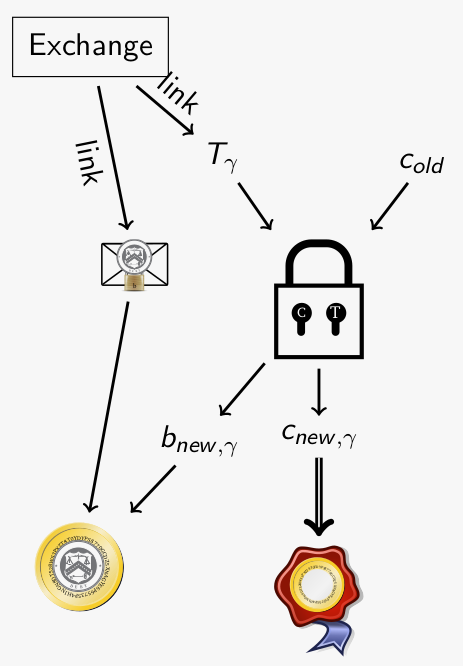
\includegraphics[height=0.5\textwidth]{taler_refresh_link_threat.png}
        \caption{Taler refresh protocol, linkability (source: \cite{pic:refresh-prot})}
        \label{fig:taler-link-threat}
    \end{figure}
    The goal of the cut and choose protocol is to ensure with a high probability ($1/n$) that the customer honestly created the new coin.
    It ensures that the old coin is linked to the new coin via the DH lock.

    With that, the following attack scenario is prevented (with probability $1/n$):\\
    An third party creates the new coin without the DH lock as described in section \ref{sec:blind-sign-schemes}.
    The third party sends the blinded new coin to the customer (who possesses the old coin).
    The customer then signs the new coin by the exchange and sends the blinded signature back to the third party.
    The third party would then be in possession of a valid new coin, which is not linked to the old coin.
    As mentioned, such an attack is detected with a high probability by the exchange with the cut and choose protocol described earlier.

    We will now consider the following attack scenario:\\
    Someone could give the private key of the old coin $c_{old}$ to another person.
    This other person then can derive a new coin using the refresh protocol.
    The original customer currently can not recreate the new coin with only the knowledge of the old coins private key $c_{old}$.
    He would need to know the public key of the transfer key $T_x$ and also the blinded signature of the new coin $f'_{new}$.
    For this reason the exchange exposes the public transfer key $T_x$ and the blinded new coin $f'_{new}$ for a given old coin $C_{old}$.
    So anybody who knows the public key of the old coin could ask for the public transfer key and the blinded signature of the new coin.
    Only a person in possession of the old coins private key $c_{old}$ can recreate the new coin's private key. \\
This mechanism can not be abused for money laundering anymore, since the original customer could trick this third person and spend the coin faster.
The linking protocol is described in figure \ref{fig:refresh-link}.

\begin{figure}
    \begin{equation*}
        \resizebox{1.0\textwidth}{!}{$\displaystyle
        \begin{array}{ l c l }
            % preliminaries
            \text{Customer} &  & \text{Exchange}
            \\ \text{knows:} & & \text{knows:}
            \\ \text{coin}_0 = \langle D_{p(0)}, c_s^{(0)}, C_p^{(0)}, \sigma_{C}^{(0)} \rangle
            \\ & \xrightarrow[\rule{2.5cm}{0pt}]{C_{p(0)}} &
            \\ & &  L := \text{LookupLink}(C_{p(0)})
            \\ & &  \textbf{Comment: } \text{LookupLink}(C_p) \mapsto \{\langle \rho_L^{(i)},
            \\ & & \sigma_L^{(i)}, \overline{\sigma}_C^{(i)} \rangle\}
            \\ & \xleftarrow[\rule{2.5cm}{0pt}]{L} &
            \\ \pcfor \langle \rho_{L}^{(i)}, \overline{\sigma}_L^{(i)}, \sigma_C^{(i)} \rangle \in L
            \\ \langle \hat{C}_p^{(i)}, D_{p(t)}^{(i)}, T_\gamma^{(i)}, \overline{m}_\gamma^{(i)} \rangle := \rho_L^{(i)}
            \\ \langle e_t^{(i)}, N_t^{(i)} \rangle := D_{p(t)}^{(i)}
            \\ \textbf{check } \hat{C}_p^{(i)} \equiv  C_p^{(0)}
            \\ \textbf{check } \text{Ed25519.Verify}(C_p^{(0)}, \rho_{L}^{(i)}, \sigma_L^{(i)})
            \\ x_i := \text{ECDH}(c_s^{(0)}, T_{\gamma}^{(i)})
            \\ r_i := \text{SelectSeeded}(x_i,\mathbb{Z}^*_{N_t})
            \\ c_s^{(i)} := \text{HKDF}(256,x_i,"c")
            \\ C_p^{(i)} := \text{Ed25519.GetPub}(c_s^{(i)})
            \\ \sigma_C^{(i)} := (r_i)^{-1} \cdot \overline{m}_\gamma^{(i)}
            \\ \textbf{check } (\sigma_C^{(i)})^{e_t^{(i)}} \equiv_{N_t^{(i)}} C_p^{(i)}
            \\ \text{(Re-)obtain coin} \langle D_{p(t)}^{(i)},c_s^{(i)}, C_p^{(i)}, \sigma_C^{(i)} \rangle
        \end{array}$
        }
    \end{equation*}
    \caption{Linking protocol}
    \label{fig:refresh-link}
\end{figure}


\subsection{Tipping Protocol}
\label{sec:tipping}
Source for this protocol was section 4.1.10 from \cite{dold:the-gnu-taler-system}.\\
Merchants can give customers a small tip by using the withdraw loophole (described in section \ref{sec:withdraw-loophole}).
This can be for a variety of different reasons, for example for submitting a survey.
The merchant needs to create a reserve with the exchange.
The reserve keys is now used to sign blinded coins generated by the user.
\begin{enumerate}
    \item The Merchant triggers the Payment required response with the Taler-Tip header set
    \item The taler tip header contains information like amount, exchange to use, deadline and more. (details section 4.1.10 \cite{dold:the-gnu-taler-system})
    \item The customer creates planchets that sum up the amount and blinds the token with the denomination key of the specified exchange and sends the blinded planchets to the merchant.
    \item The merchant creates withdrawal confirmations (by signing them with the reserver private key) for these planchets and responds with a list of signatures.
    \item The customer then uses these signatures to create coins as in the withdrawal protocol
\end{enumerate}
The received coins are still anonymized and only spendable by the customer.


\subsection{Refund Protocol}
A merchant can undo a deposit on a coin by signing a refund permission.
The protocol details can be found in section 4.7.5 of \cite{dold:the-gnu-taler-system}.
Since a refund is mainly done by the merchant, to provide refunds a merchant need to support refunds.
A refund can be either fully or partially.
After a refund, the customer is able to spend the coin, but it should be refreshed first to prevent linking of transactions.
The refund deadline is specified in the contract header, after the deadline the exchange makes a wire transfer with the money to the merchants bank.
There is a refund fee, which is subtracted from the remaining coin value.
This also prevents denial of service attacks, or at least makes them economically uninteresting.
There exists automatic refunds when a payment only partially succeeds for many reasons.
Refunds are also an important business case for many merchants who want to provide a convenient experience.
A merchant can for example provide a refund when the customer is not happy with the product.
Such a refund can be made by the merchant with a signature without the customers consent.
Now should be clear what the purpose of a refund protocol is, the rest of this section will look at the refund protocol.


In the protocol the customer requests a refund from the merchant.
If the merchant accepts the request, it authorizes the exchange to apply the refund.
\begin{enumerate}
    \item The customer asks for a refund for payment $p$ with reason $m$
    \item The merchant decides whether it accepts the refund or not according to the merchants business rules.
    \item If accepted, the merchant signs the refund permission with the merchants Ed25519 key and sends it to exchange.
    \item The exchange checks the signature and refunds the coin(s) and sends a signed confirmation to the merchant.
    \item The merchant sends the signed confirmation from the exchange to the customer.
\end{enumerate}

\section{Trust and PKI in Taler}
In this section Taler's \ac{PKI} is explained and how Taler handles trust.
This section is included due to the reason that we have to create Schnorr denomination keys to add the Clause Blind Schnorr Signature scheme to Taler.
Taler uses TLS, however it does not rely on TLS for authenticity or integrity. (More detailed in chapter 4.1.3 of \cite{dold:the-gnu-taler-system})

\subsubsection{Auditor}
In Taler the auditors serves as trust anchor, and they are identified by a single Ed25519 public key.
Similar to the list of trusted root \ac{CA} that come with web browsers and operating systems, a wallet comes with a list of trusted auditor certificates.
In the rest of this section, different parts of Taler and how they are integrated in Taler's \ac{PKI} are discussed.
The section ends with a discussion about security risks of Taler's trust model.
For details, refer to chapter 4.1.3 of \cite{dold:the-gnu-taler-system}.

\begin{figure}[htp]
    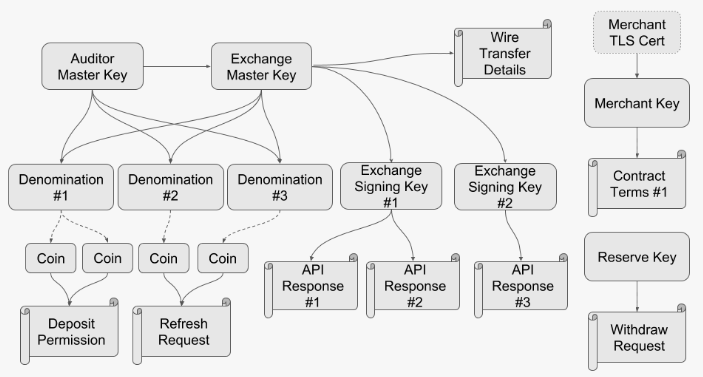
\includegraphics[height=0.5\textwidth]{taler-pki.png}
    \centering
    \caption{GNU Taler PKI entities (source: \cite{dold:the-gnu-taler-system})}
    \label{fig:taler-pki}
\end{figure}

\subsubsection{Exchange}
The exchange has to expose an API in order to enable customers (wallets), merchants and auditors to access keys and other information.
An exchange has a long term master key (Ed25519 key) and a base URL.
The URL and the long term \ac{MK} identifies an exchange.
The \ac{MK} is only used as an offline signing key and should be stored on an air-gapped machine.
Further, the exchange has online signing keys (Ed25519 key), which are signed by the exchanges \ac{MK}.
This \ac{MK} is on his side signed by one or possibly more auditors master key(s).
The exchange's (online) signing keys are used to sign API responses.
The denomination keys of an exchange are also signed by the exchanges offline \ac{MK} and the auditors \ac{MK}.
The bank accounts supported by the exchange for withdrawals and deposits are also signed by the exchanges offline \ac{MK}.

API requests are made to the base URL appending the name of the endpoint (eg. <base-url>/keys)
The endpoint <base-url>/keys is used to get the exchanges signing keys and other information.
Similar to the \ac{CA} trust model, the client (customer or merchant) can validate the signature of the keys, with the list of trusted auditor certs.

\subsubsection{Coins}
As seen in the withdrawal protocol blind signatures are done with RSA public keys (section \ref{sec:blind-rsa-sign}).
These keys are called denomination keys and they represent the coin value of the signed coins.
The following information concerning the denomination keys are signed by the exchanges master key (citation from \cite{dold:the-gnu-taler-system} chapter 4.1.3):
\begin{itemize}
    \item The RSA public key
    \item The start date, after which coins of this denomination can be withdrawn and deposited.
    \item The  withdraw  expiration  date,  after  which  coins  cannot  be  withdrawn anymore, must be after the start date.
    \item The deposit expiration date, after which coins cannot be deposited anymore, must be after the withdraw expiration date.
    \item The legal expiration date, after which the exchange can delete all records about operations with coins of this denominations, must be (typically quite a long time!) after the deposit expiration date.
    \item The fees for a withdraw, deposit, refresh and refund operation with this coin, respectively.
\end{itemize}

As mentioned, the denomination keys are signed by the exchanges \ac{MK} and also by the auditor.

\subsubsection{Merchant}
The merchant has one Ed25519 public key.
With that key the merchant authenticates to the exchange and signs responses to the customer.
Depending on the jurisdiction, an exchange needs to comply to \ac{KYC} regulations.
A merchant which accepts payments from all exchanges (audited by a trusted auditor) therefore needs to fulfill \ac{KYC} registration for all accepted exchange separately.
This is needed to be legally compliant. \\
Like the customer, also the merchant is configured with a set of trusted auditors and exchanges.
A merchant only accepts payments with coins of denominations from a trusted exchange which is audited by a trusted auditor.

For this reason Taler separates this service into an isolated service, similar to on-premise or external payment gateways, which are used by most e-commerce shops nowadays.

\subsubsection{Customer}
A customer has private keys of reserves that they own to authenticate with the exchange.
The public key was communicated to the exchange with the wire transfer. (A bank however is not part of Taler's \ac{PKI}.)
A customer is therefore not registered with an exchange.

Further a customer possesses the private keys of his coins and stores them in a digital wallet.
\subsubsection{Security Discussion}
Taler's trust model is technically similar to the \ac{CA} trust model we know from TLS certificates.
The trust anchor lies with the auditors, whose certificates are pre-configured by the merchant or customer respectively.
However, trust is always somehow attackable.
That does not mean that there is a security issue in the trust model.
When the list of trusted auditor certs of a customer/merchant somehow can be manipulated, the trust model breaks for this entity. \\
One attack scenario would be to attack customers/merchants with a supply-chain attack on the wallets or merchant backends' implementation.
With software supply-chain attacks on the rise in 2020/21 (although the concept is not new) such an attack could have a big impact. \\
Since auditor certs are coupled with the wallet (or merchant) implementation, a bank, country, central bank or auditor will most likely publish a wallet and a merchant implementation for the corresponding Taler ecosystem.
%This would make it possible for the publisher to make changes on the Taler protocol for this specific implementation.

%------------ Execution
\chapter{Protocol Design}
\label{chap:design}
This chapter describes the necessary changes on the protocol level to implement a Blind Schnorr Signature Scheme to Taler.


\section{Analysis of Current Protocols}
The blind RSA signature scheme is only used for coin signatures.
Note that we omitted protocols (or parts of them) where the coin signature is transmitted, but no other actions using it is performed.
\\\\
\label{abort-idempotency}
An important property to mention here is \textit{\gls{abort-idempotency}}.
\Gls{idempotence} in the context of computer science is a property to ensure that the state of a system will not change, no matter how many times the same request was made.
A more in-depth explanation is given within the cited source \cite{yuchen:idempotence}.\\
\textit{\gls{abort-idempotency}} goes a bit further.
When the protocol is aborted at any stage, for example due to power cuts or network issues, the protocol still needs to ensure that the same response is sent for the same request.
This is especially challenging when dealing with random values as we will see in the redesigned protocols in the following sections.
For \gls{RSABS} it is inherently easier to provide \textit{\gls{abort-idempotency}} since signature creation only needs one round-trip and requires less random values.

The following protocols currently use \gls{RSABS}:
\begin{itemize}
    \item \textbf{Withdraw Protocol:}
          The customer uses the blind signature scheme to blind the coins before transmitting them to the exchange, which blindly signs it (standard RSA signature) and the returns the signatures.
          After the customer receives the signatures, he unblinds and stores them together with the coins.
          \\ Components:
          \begin{itemize}
              \item Customer
              \item Exchange
          \end{itemize}
    \item \textbf{Deposit Protocol:}
          During the Deposit, the exchange verifies the coin signature derived using the blind RSA signature scheme.
          \\ Components:
          \begin{itemize}
              \item Exchange
          \end{itemize}
    \item \textbf{Refresh Protocol:}
          The refresh protocol is used to derive a new coin from an old one which was partially spent.
          Parts of the protocol are similar to the withdraw protocol, but it is more complex due to the added DH lock and cut-and-choose.
          \\ Components:
          \begin{itemize}
              \item Customer
              \item Exchange
          \end{itemize}
    \item \textbf{Tipping:}
          Tipping is a variation of the withdraw protocol where the message containing the blinded planchets is transmitted to the merchant, who signs them using his reserve private, key and returns the signatures back to the customer.
          Here, the details from the withdraw protocol apply.
          \\ Components:
          \begin{itemize}
              \item Customer
              \item Exchange
          \end{itemize}
    \item \textbf{Payback Protocol:}
          The payback protocol distinguishes three different cases, which either use the refresh protocol or disclose either the withdraw transcript or refresh protocol transcript to the exchange.
          \\ Components:
          \begin{itemize}
              \item Customer
              \item Exchange
          \end{itemize}
\end{itemize}


\section{Protocol Changes}
The goal of the thesis is to add support for the Clause Blind Schnorr Signature scheme to Taler, besides the existing \gls{RSABS} implementation (see section \ref{sec:blind-rsa-sign}).
For the design of the \gls{CSBS} the existing protocols with \gls{RSABS} were redesigned.

The goal of the blind signature is to keep the exchange from knowing which coin a user withdraws and thus preventing the exchange linking a coin to a user.
The biggest impact is on the withdrawal and refresh protocols, but all protocols that include some operation around denomination signatures are affected.

During the thesis the protocols will be redesigned, implemented and the differences to the current version will be outlined.
These results will be delivered to the Taler team.
Feedback is very important when (re)designing protocols.
For that reason the redesigned protocols were discussed and reviewed with Christian Grothoff multiple times.

As signature scheme the Clause Blind Schnorr Signature Scheme described in section \ref{sec:clause-blind-schnorr-sig} was chosen for multiple reasons.
First of all it is currently considered to be secure (see \cite{cryptoeprint:2019:877}).
Schnorr Signatures on \gls{25519} are much shorter than RSA signatures.
This should provide notable performance improvements in speed and storage, and therefore scales better.
The paper describes a security analysis of the Blind Schnorr Signature scheme and introduces a modification (the "clause" part in the name) that is resistant to Wagner's algorithm (which solves ROS problem).

\Gls{25519} \cite{bern:curve25519} will be used for the implementation because it is a widely accepted curve (see \cite{bernlange:safecurves}, \cite{rfc7748}) and is already used by Taler (Taler uses Ed25519 which is built upon \gls{25519}).


\subsection{Withdraw Protocol}
\label{sec:withdraw-protocol-schnorr}
The modified protocol using the Clause Blind Schnorr Signature Scheme is described in figures \ref{fig:withdrawal-process-schnorr-1} and \ref{fig:withdrawal-process-schnorr-2}.

The proposed change introduces an additional round trip.
It must be prevented that the exchange has to track sessions or persist values during the first stage \ref{fig:withdrawal-process-schnorr-1}, while still ensuring \gls{abort-idempotency}.
In order to ensure \textit{\gls{abort-idempotency}}, the exchange has to generate the same $R_0,R_1$ for the same withdrawal request, while $r_0,r_1$ still needs to be unpredictable for the customer.
For this reason a withdrawal-nonce combined with a \gls{hkdf} comes into play.
The redesigned protocol makes extensive use of \gls{hkdf}'s functionality as \ac{PRNG} and one-way function, thus random becomes \textit{unpredictable}.

In the beginning of the protocol, the customer generates a coin key pair.
Its private key is used to generate the withdraw-nonce $n_w$ and the blinding factors $\alpha_0, \alpha_1, \beta_0, \beta_1$.
The exchange uses the withdraw nonce together with the reserve key and a long-term secret to generate $r_0, r_1$.
The coin and denomination private keys can be used as long-term secrets due to the one-way property of the \gls{hkdf}.

Another question evolved around which key to use for the derivation of $ r_0, r_1 $.
Obvious options are the denomination key or the exchange's online signing key.
The denomination key was chosen because it has the payback protocol in place that would handle coin recovery in case of a key compromise and subsequent revocation.

\begin{figure}[htp]
  \begin{equation*}
    \resizebox{1.0\textwidth}{!}{$\displaystyle
    \begin{array}{ l c l }
      % preliminaries
      \text{Customer} &  & \text{Exchange}
      \\ \text{knows:} & & \text{knows:}
      \\ \text{reserve keys } w_s, W_p & & \text{reserve public key } W_p
      \\ \text{denomination public key } D_p & & \text{denomination keys } d_s, D_p
      \\ & &
      \\\text{generate withdraw secret:}
      \\ \omega := randombytes(32)
      \\ \text{persist } \langle \omega, D_p \rangle
      \\ n_w := \text{HKDF}(256, \omega,\text{"n"})
      \\ & \xrightarrow[\rule{2.5cm}{0pt}]{n_w, D_p} &
      % generate R
      \\ & & \text{verify if } D_p \text{ is valid}
      \\ & & r_0 := \text{HKDF}(256,n_w || d_s, \text{"r0"})
      \\ & & r_1 := \text{HKDF}(256,n_w || d_s, \text{"r1"})
      \\ & & R_0 := r_0G
      \\ & & R_1 := r_1G
      \\ & \xleftarrow[\rule{2.5cm}{0pt}]{R_0, R_1} &
      \\ \text{derive coin key pair}:
      \\ c_s := \text{HKDF}(256, \omega || R_0 || R_1,\text{"cs"})
      \\ C_p := \text{Ed25519.GetPub}(c_s)
      % blinding
      \\ \text{blind:} & &
      \\ b_s := \text{HKDF}(256, \omega || R_0 || R_1,\text{"b-seed"})
      \\ \alpha_0 := \text{HKDF}(256, b_s, \text{"a0"})
      \\ \alpha_1 := \text{HKDF}(256, b_s, \text{"a1"})
      \\ \beta_0 := \text{HKDF}(256, b_s, \text{"b0"})
      \\ \beta_1 := \text{HKDF}(256, b_s, \text{"b1"})
      \\ R'_0 := R_0 + \alpha_0 G + \beta_0 D_p & &
      \\ R'_1 := R_1 + \alpha_1 G + \beta_1 D_p & &
      \\ c'_0 := H(R'_0, C_p) & &
      \\ c'_1 := H(R'_1, C_p) & &
      \\ c_0 := c'_0 + \beta_0 \mod p & &
      \\ c_1 := c'_1 + \beta_1 \mod p & &
      \\
      \\ & \textit{Continued in figure \ref{fig:withdrawal-process-schnorr-2}} &
    \end{array}$
    }
  \end{equation*}
  \caption{Withdrawal process using Clause Blind Schnorr Signatures part 1}
  \label{fig:withdrawal-process-schnorr-1}
\end{figure}

\begin{figure}[htp]
  \begin{equation*}
    \resizebox{1.0\textwidth}{!}{$\displaystyle
    \begin{array}{ l c l }
      % preliminaries
      \text{Customer} &  & \text{Exchange}
      \\ \text{knows:} & & \text{knows:}
      \\ \text{reserve keys } w_s, W_p & & \text{reserve public key } W_p
      \\ \text{denomination public key } D_p & & \text{denomination keys } d_s, D_p
      \\
      \\ & \textit{Continuation of figure \ref{fig:withdrawal-process-schnorr-1}} &
      \\
      % sign with reserve sk
      \\ \text{sign with reserve private key:} & &
      \\ \rho_W := \langle n_w, D_p, c_0, c_1 \rangle & &
      \\ \sigma_W := \text{Ed25519.Sign}(w_s, \rho_W) & &
      \\ & \xrightarrow[\rule{2.5cm}{0pt}]{W_p, \sigma_W, \rho_W} &
      \\ & & \langle n_w, D_p, c_0, c_1 \rangle := \rho_W
      % checks done by the exchange
      \\ & & \text{verify if } D_p \text{ is valid}
      \\ & & \text{check } \text{Ed25519.Verify}(W_p, \rho_W, \sigma_W)
      \\ & & b := \text{HKDF}(1,n_w || d_s, \text{"b"})
      \\ & & s \leftarrow \text{GetWithdraw}(n_w, D_p)
      \\ & & \textbf{if } s = \bot
      \\ & & r_b := \text{HKDF}(256,n_w || d_s, \text{"r}b\text{"})
      % sign coin
      \\ & & s := r_b + c_b d_s \mod p
      % the following db operations are atomic
      \\ & & \text{decrease balance if sufficient and}
      \\ & & \text{persist } \langle n_w, D_p, s \rangle
      \\ & & \textbf{endif}
      \\ & \xleftarrow[\rule{2.5cm}{0pt}]{b,s} &
      % verify signature
      \\ \text{verify signature:}& &
      \\ \textbf{check if } sG = R_b + c_b D_p & &
      % unblind signature
      \\ \text{unblind:}& &
      \\ s' := s + \alpha_b \mod p & &
      \\ \text{verify signature:}& &
      \\ \textbf{check if } s'G = R'_b + c'_b D_p & &
      \\ \sigma_C := \langle R'_b, s' \rangle & &
      \\ \text{resulting coin: } c_s, C_p, \sigma_C, D_p & &
      
    \end{array}$
    }
  \end{equation*}
  \caption{Withdrawal process using Clause Blind Schnorr Signatures part 2}
  \label{fig:withdrawal-process-schnorr-2}
\end{figure}


\subsection{Deposit Protocol}
The deposit protocol remains unchanged, except for the verification of the coin signature.
To verify the signature, the exchange has to check if the following equation holds:
\begin{align*}
  s'G & = R' + c' D_p
  \\ &= R' + H(R', C_p) D_p
\end{align*}
$ s', R' $ together form the signature, $ D_p $ is the denomination public key and $ C_p $ is the coin public key.

Further details regarding the verification process can be found in section \ref{sec:blind-schnorr-sig}.


\subsection{Refresh Protocol}
The refresh protocol blindly signs the new derived coins.
The replacement of \gls{RSABS} with the Clause Blind Schnorr Signature Scheme (see \ref{sec:clause-blind-schnorr-sig}) makes the refresh protocol a bit more complex.

\subsubsection{RefreshDerive Schnorr}
The RefreshDerive protocol is described in figure \ref{fig:refresh-derive-schnorr}.
For this protocol, the main change is that more values need to be derived somehow.
These blinding factors are also derived from $x$.
Then the challenges $\overline{c_0}$ and $\overline{c_1}$ are generated as in the Clause Blind Schnorr Signature Scheme.

\begin{figure}[htp]
  \centering
  \fbox{%
    \procedure[codesize=\small]{$\text{RefreshDerive}(t, D_{p(t)}, C_p, R_0, R_1)$}{%
      T := \text{Curve25519.GetPub}(t) \\
      x := \textrm{ECDH-EC}(t, C_p)  \\
      c'_s := \text{HKDF}(256, x, \text{"c"}) \\
      C_p' := \text{Ed25519.GetPub}(c'_s)  \\
      b_s := \text{HKDF}(256, x || R_0 || R_1,\text{"b-seed"}) \\
      \alpha_0 := \text{HKDF}(256, b_s, \text{"a0"}) \\
      \alpha_1 := \text{HKDF}(256, b_s, \text{"a1"}) \\
      \beta_0 := \text{HKDF}(256, b_s, \text{"b0"}) \\
      \beta_1 := \text{HKDF}(256, b_s, \text{"b1"}) \\
      R'_0 = R_0 + \alpha_0 G + \beta_0 D_p \\
      R'_1 = R_1 + \alpha_1 G + \beta_1 D_p \\
      c'_0 = H(R'_0, C_p') \\
      c'_1 = H(R'_1, C_p') \\
      \overline{c_0} = c'_0 + \beta_0 \mod p \\
      \overline{c_1} = c'_1 + \beta_1 \mod p \\
      \pcreturn \langle T, c'_s, C_p', \overline{c_0}, \overline{c_1} \rangle
    }
  }
  \caption[RefreshDerive algorithm]{The RefreshDerive replaced with Schnorr blind signature details. As before the uses the seed $s$ on the dirty coin for generating the new coin.
    The new coin needs to be signed later on with the denomination key.}
  \label{fig:refresh-derive-schnorr}
\end{figure}

\subsubsection{Refresh Protocol}
\label{sec:refresh-protocol}
In the commit phase (see figure \ref{fig:refresh-commit-part1}) there needs to be requested an $R_0$ and $R_1$ before deriving the new coins.
There now needs to be calculated two different commit hashes, one for $\overline{c_0}$ and one for $\overline{c_1}$.
The exchange needs to additionally generate a random $b \leftarrow \{0,1\}$ to choose a $\overline{c_b}$.
The reveal phase (see figure \ref{fig:refresh-commit-part2}) now is continued only with the chosen $\overline{c_b}$.
In the reveal phase, the RSA signing and unblinding is exchanged with Schnorr's blind signature counterparts.

\begin{figure}[htp]
  \begin{equation*}
    \resizebox{1.0\textwidth}{!}{$\displaystyle
    \begin{array}{ l c l }
      % preliminaries
      \text{Customer} &  & \text{Exchange}
      \\ \text{knows:} & & \text{knows:}
      \\ \text{denomination public key } D_p & & \text{old denomination keys } d_{s(0)} D_{p(0)}
      \\ \text{coin}_0 = \langle D_{p(0)}, c_s^{(0)}, C_p^{(0)}, \sigma_c^{(0)} \rangle  &&  \text{new denomination keys } d_s, D_P
      % request r
      \\ & &
      \\ \omega := randombytes(32)
      \\ \text{persist } \langle \omega, D_p \rangle
      %\\ s_w := \text{HKDF}(256,  c_s^{(0)},\text{"n"})
      \\ n_r := \text{HKDF}(256, \omega,\text{"n"})
      % sign with reserve sk
      \\ & \xrightarrow[\rule{2.5cm}{0pt}]{n_r, D_p} &
      % generate R
      \\ & & \text{verify if } D_p \text{ is valid}
      \\ & & r_0 := \text{HKDF}(256,n_r || d_s, \text{"r0"})
      \\ & & r_1 := \text{HKDF}(256,n_r || d_s, \text{"r1"})
      \\ & & R_0 := r_0G
      \\ & & R_1 := r_1G
      \\ & \xleftarrow[\rule{2cm}{0pt}]{R_0, R_1} &
      % refresh request
      \\ \textbf{for } i = 1, \dots, \kappa: % generate k derives
      %\\ s_i \leftarrow \{0,1\}^{256} % seed generation
      \\ t_i := \text{HKDF}(256, \omega || R_0 || R_1,\text{"t} i \text{"} )  % seed generation
      \\ X_i := \text{RefreshDerive}(t_i, D_p, C_p^{(0)}, R_0, R_1)
      \\ (T_i, c_s^{(i)}, C_p^{(i)}, \overline{c_0}, \overline{c_1}):= X_i
      \\ \textbf{endfor}
      \\ h_T := H(T_1, \dots, T_k)
      \\ h_{\overline{c_0}} := H(\overline{c_{0_1}},\dots, \overline{c}_{0_k})
      \\ h_{\overline{c_1}} := H(\overline{c_{1_1}},\dots, \overline{c}_{1_k})
      \\ h_{\overline{c}} := H(h_{\overline{c_0}}, h_{\overline{c_1}})
      \\ h_C := H(h_T, h_{\overline{c}})
      \\ \rho_{RC} := \langle h_C, D_p, \text{ } D_{p(0)}, C_p^{(0)}, \sigma_C^{(0)}  \rangle
      \\ \sigma_{RC} := \text{Ed25519.Sign}(c_s^{(0)}, \rho_{RC})
      \\ \text{Persist refresh-request}
      \\ \langle \omega, R_0, R_1, \rho_{RC}, \sigma_{RC} \rangle
      \\
      \\ & \textit{Continued in figure \ref{fig:refresh-commit-part2}} &
    \end{array}$
    }
  \end{equation*}
  \caption{Refresh protocol (commit phase part 1) using Clause Blind Schnorr Signatures}
  \label{fig:refresh-commit-part1}
\end{figure}


\begin{figure}[htp]
  \begin{equation*}
    \resizebox{1.0\textwidth}{!}{$\displaystyle
    \begin{array}{ l c l }
      \text{Customer} &  & \text{Exchange}
      \\ & \textit{Continuation of}
      \\ & \textit{figure \ref{fig:refresh-commit-part1}}
      \\
      \\ & \xrightarrow[\rule{2cm}{0pt}]{\rho_{RC}, \sigma_{RC}} &
      % Exchange checks refresh request
      \\ & & \langle h_C, D_p, D_{p(0)}, C_p^{(0)}, \sigma_C^{(0)} \rangle := \rho_{RC}
      \\ & & \textbf{check} \text{ Ed25519.Verify}(C_p^{(0)}, \sigma_{RC}, \rho_{RC})
      \\
      \\ & & \gamma \leftarrow \text{GetOldRefresh}(\rho_{RC})
      \\ & & \textbf{Comment: }\text{GetOldRefresh}(\rho_{RC} \mapsto
      \\ & & \{\bot, \gamma \})
      \\ & & \pcif \gamma = \bot
      \\ & & v := \text{Denomination}(D_p)
      \\ & & \textbf{check } \text{IsOverspending}(C_p^{(0)}, D_ {p(0)}, v)
      \\ & & \text{verify if } D_p \text{ is valid}
      \\ & & \textbf{check } \text{Schnorr.Verify}(D_{p(0)}, C_p^{(0)}, \sigma_C^{(0)})
      \\ & & \text{MarkFractionalSpend}(C_p^{(0)}, v)
      \\ & & \gamma \leftarrow \{1, \dots, \kappa\}
      \\ & & \text{Persist refresh-record } \langle \rho_{RC},\gamma \rangle
      \\ & \xleftarrow[\rule{2cm}{0pt}]{\gamma} &
      % Check challenge and send challenge response (reveal not selected msgs)
      \\ \textbf{check } \text{IsConsistentChallenge}(\rho_{RC}, \gamma)
      \\ \textbf{Comment: } \text{IsConsistentChallenge}\\(\rho_{RC}, \gamma) \mapsto \{ \bot,\top \}
      \\
      \\ \text{Persist refresh-challenge} \langle \rho_{RC}, \gamma \rangle
      \\ S := \langle t_1, \dots, t_{\gamma-1}, t_{\gamma+1}, \dots,t_\kappa \rangle % all seeds without the gamma seed
      \\ \rho_L := \langle C_p^{(0)}, D_p, T_{\gamma}, \overline{c_0}_\gamma, \overline{c_1}_\gamma, n_r \rangle
      \\ \rho_{RR} := \langle \rho_L, S \rangle
      \\ \sigma_{L} := \text{Ed25519.Sign}(c_s^{(0)}, \rho_{L})
      \\ & \xrightarrow[\rule{2.5cm}{0pt}]{\rho_{RR},\rho_L, \sigma_{L}} &
      \\
      \\ & \textit{Continued in} &
      \\ & \textit{figure \ref{fig:refresh-reveal-part1}} &
    \end{array}$
    }
  \end{equation*}
  \caption{Refresh protocol (commit phase part 2) using Clause Blind Schnorr Signatures}
  \label{fig:refresh-commit-part2}
\end{figure}

\begin{figure}[htp]
  \begin{equation*}
    \resizebox{1.0\textwidth}{!}{$\displaystyle
    \begin{array}{ l c l }
      % preliminaries
      \text{Customer} &  & \text{Exchange}
      \\ & \textit{Continuation of}
      \\ & \textit{figure \ref{fig:refresh-commit-part2}}
      \\
      \\ & \xrightarrow[\rule{2.5cm}{0pt}]{\rho_{RR},\rho_L, \sigma_{L}} &
      % check revealed msgs and sign coin
      \\ & & \langle C_p^{(0)}, D_p, T_{\gamma}, \overline{c_0}_\gamma, \overline{c_1}_\gamma, n_r \rangle := \rho_L
      \\ & & \langle T'_\gamma, \overline{c_0}_\gamma, \overline{c_1}_\gamma, S \rangle := \rho_{RR}
      \\ & & \langle t_1,\dots,t_{\gamma-1},t_{\gamma+1},\dots,t_\kappa \rangle := S
      \\ & & \textbf{check } \text{Ed25519.Verify}(C_p^{(0)}, \sigma_L, \rho_L)
      \\ & & b := \text{HKDF}(1,n_r || d_{s(i)}, \text{"b"})
      \\ & & \textbf{for } i = 1,\dots, \gamma-1, \gamma+1,\dots, \kappa
      \\ & & X_i := \text{RefreshDerive}(t_i, D_p, C_p^{(0)} \\ &&, R_0, R_1)
      \\ & & \langle T_i, c_s^{(i)}, C_p^{(i)}, \overline{c_1}_i, \overline{c_2}_i \rangle := X_i
      \\ & & \textbf{endfor}
      \\ & & h_T' = H(T_1,\dots,T_{\gamma-1},T'_{\gamma},T_{\gamma+1},\dots,T_\kappa)
      \\ & & h_{\overline{c_0}}' := H(\overline{c_{0_1}},\dots, \overline{c}_{0_k})
      \\ & & h_{\overline{c_1}}' := H(\overline{c_{1_1}},\dots, \overline{c}_{1_k})
      \\ & & h_{\overline{c}}' := H(h_{\overline{c_0}}, h_{\overline{c_1}})
      \\ & & h_C' = H(h_T', h_{\overline{c}}')
      \\ & & \textbf{check } h_C = h_C'
      \\ & & r_b := \text{HKDF}(256,n_r || d_s, \text{"r}b\text{"})
      \\ & & \overline{s}_{C_p}^{(\gamma)} = r_b + \overline{c_{b_\gamma}} d_s \mod p
      \\ & & \text{persist } \langle \rho_L, \sigma_L \rangle
      \\ & \xleftarrow[\rule{2.5cm}{0pt}]{b, \overline{s}_C^{(\gamma)}} &
      % Check coin signature and persist coin
      % unblind signature
      \\ \text{unblind:}& &
      \\ s_C'^{(\gamma)} := \overline{s}_C^{(\gamma)} + \alpha_b \mod p & &
      \\ \text{verify signature:}& &
      \\ \textbf{check if } \overline{s'}_C^{(\gamma)}G \equiv R'_b + \overline{c'_0}_\gamma D_p & &
      \\ \sigma_C^{(\gamma)} := \langle s_{C}'^{(\gamma)},R_b' \rangle
      \\ \text{Persist coin} \langle D_p, c_s^{(\gamma)}, C_p^{(\gamma)}, \sigma_C^{(\gamma)} \rangle
    \end{array}$
    }
  \end{equation*}
  \caption{Refresh protocol (reveal phase) using Clause Blind Schnorr Signatures}
  \label{fig:refresh-reveal-part1}
\end{figure}
\newpage
\subsubsection{Linking Protocol}
\label{sec:refresh-link}
The beginning of the linking protocol (see figure \ref{fig:refresh-link}) is the same as in the current protocol.
After the customer received the answer $L$ the only difference is in obtaining the coin.
To re-obtain the derived coin, the same calculations as in \ref{fig:refresh-derive-schnorr} are made.
\begin{figure}[htp]
  \begin{equation*}
    \resizebox{1.0\textwidth}{!}{$\displaystyle
    \begin{array}{ l c l }
      % preliminaries
      \text{Customer} &  & \text{Exchange}
      \\ \text{knows:} & & \text{knows:}
      \\ \text{coin}_0 = \langle D_{p(0)}, c_s^{(0)}, C_p^{(0)}, \sigma_{C}^{(0)} \rangle
      \\ & \xrightarrow[\rule{2.5cm}{0pt}]{C_{p(0)}} &
      \\ & &  L := \text{LookupLink}(C_{p(0)})
      \\ & &  \textbf{Comment: } \text{LookupLink}(C_p^{(0)}) \mapsto 
      \\ & & \{\langle \rho_L^{(i)}, \sigma_L^{(i)}, \overline{\sigma}_C^{(i)}, b \rangle\}
      %\\ & & \{\langle C_{p(0)}, D_{p(t)},\overline{\sigma}_C^{(i)}, b^{(i)}, R_b^{(i)}\rangle\}
      \\ & \xleftarrow[\rule{2.5cm}{0pt}]{L} &
      \\ \textbf{for } \langle \rho_L^{(i)}, \overline{\sigma}_L^{(i)}, \overline{\sigma}_C^{(i)}, b \rangle\ \in L
      
      %\\ & & \langle C_p^{(0)}, D_{p(t)}, T_{\gamma}, \overline{c_0}_\gamma, \overline{c_1}_\gamma, n_r \rangle := \rho_L
      \\ \langle \hat{C}_p^{(i)}, D_p^{(i)}, T_\gamma^{(i)}, \overline{c_0}_\gamma^{(i)}, \overline{c_1}_\gamma^{(i)}, n_r \rangle := \rho_L^{(i)}
      \\ \langle \overline{s}_C^{(i)}, R_b^{(i)} \rangle := \overline{\sigma}_C^{(i)}
      \\ \textbf{check } \hat{C}_p^{(i)} \equiv  C_p^{(0)}
      \\ \textbf{check } \text{Ed25519.Verify}(C_p^{(0)}, \rho_{L}^{(i)}, \sigma_L^{(i)})
      \\ \langle \overline{s}_C^{(i)}, R_b^{(i)} \rangle := \sigma_C^{(i)}
      \\ x_i := \text{ECDH}(c_s^{(0)}, T_{\gamma}^{(i)})
      \\ c_s^{(i)} := \text{HKDF}(256, x, \text{"c"})
      \\ C_p^{(i)} := \text{Ed25519.GetPub}(c_s^{(i)})
      \\ b_s^{(i)} := \text{HKDF}(256, x_i || R_0^{(i)} || R_1^{(i)},\text{"b-seed"})
      \\ \alpha_b := \text{HKDF}(256, b_s^{(i)}, \text{"a}b\text{"})
      \\ \beta_b := \text{HKDF}(256, b_s^{(i)}, \text{"b}b\text{"})
      \\ {R'}_b^{(i)} = R_b^{(i)} + \alpha_b G + \beta_b D_p^{(i)}
      \\ c'_b = H(R'_b, C_p^{(i)})
      \\ c_b = c'_b + \beta_b \mod p
      \\ s_C'^{(i)} := \overline{s}_C^{(i)} + \alpha_b \mod p
      \\ \sigma_C^{(i)} := \langle s_C'^{(i)}, R_b' \rangle
      \\ \textbf{check } s'{_C^{(i)}}G \equiv {R'}_b^{(i)} + c'_b D_p^{(i)}
      \\ \text{(Re-)obtain coin} \langle D_p^{(i)},c_s^{(i)}, C_p^{(i)}, \sigma_C^{(i)} \rangle
    \end{array}$
    }
  \end{equation*}
  \caption{Linking protocol using Clause Blind Schnorr Signatures}
  \label{fig:refresh-link}
\end{figure}


\subsection{Tipping}
Tipping remains unchanged, except for the content of the message $ \rho_W = D_p, c_0, c_1 $ signed by the merchant using its reserve private key.

\subsection{Payback Protocol}
The payback protocol distinguishes three different cases, which all depend on the state of a coin whose denomination key has been revoked.
The following listing outlines the necessary changes on the protocol, please refer to Dold's documentation section 2.2.1 \cite{dold:the-gnu-taler-system} for details regarding the different cases.
\begin{itemize}
  \item \textbf{The revoked coin has never been seen by the exchange}:
        \\The withdraw transcript (and verification) must be adjusted in order for the exchange to be able to retrace the blinding.
  \item \textbf{The coin has been partially spent}:
        \\In this case the refresh protocol will be invoked on the coin.
        The necessary changes are outlined in \ref{sec:refresh-protocol}.
  \item \textbf{The revoked coin has never been seen by the exchange and resulted from a refresh operation}:
        \\The refresh protocol transcript and its blinding factors must be adjusted to consider the changes in the blind signature scheme.
\end{itemize}


\chapter{Protocol Specification}
\label{chap:spec}
The proposed Taler protocols using the Clause Blind Schnorr Signature Scheme will be implemented as an additional option besides the existing \gls{RSABS} variant of the protocol as suggested by Christian Grothoff.
A Taler Exchange operator should be able to configure whether he wants to use \gls{RSABS} or \gls{CSBS}.
\\This variant allows to choose the signature scheme globally or per denomination.
Furthermore, it allows a change of signature scheme in a non-breaking way by revoking (or letting expire) a denomination and offering new denominations with the other scheme.
\\
The following key points are specified in this chapter:
\begin{itemize}
  \item Architecture of the different components
  \item Explain and specify needed changes
  \item Data strucutures
  \item Public \acp{API}
  \item Persistence
  \item Used libraries
\end{itemize}

\section{Architecture}
Before specifying the implementation of the different protocols, a deeper understanding of the technical architecture of Talers components is needed.
this section introduces the architecture of the exchange and wallet components and explains where the needed changes need to be implemented on a high-level.

\subsection{Exchange}
An introduction to the exchange can be found in section \ref{sec:exchange}.
An exchange operator needs to run and maintain some additional services besides Taler's exchange.
Although this is not directly relevant for the implementation, it helps to better understand the environment in which the exchange runs.
The perspective of an exchange operator can be seen in figure \ref{fig:taler:exchange-operator-architecture}.

\begin{figure}[h!]
  \begin{adjustbox}{max totalsize={.9\textwidth}{.7\textheight},center}
    \begin{tikzpicture}
      \tikzstyle{def} = [node distance= 5em and 6.5em, inner sep=1em, outer sep=.3em];
      \node (origin) at (0,0) {};
      \node (exchange) [def,above=of origin,draw]{Exchange};
      \node (nexus) [def, draw, below right=of exchange] {Nexus};
      \node (corebanking) [def, draw, below left=of nexus] {Core Banking};
      \node (nginx) [def, draw, above=of exchange]{Nginx};
      \node (postgres) [def, draw, below left=of exchange]{Postgres};
      \node (postgres-nexus) [def, draw, below right=of nexus]{Postgres};

      \tikzstyle{C} = [color=black, line width=1pt]

      \draw [<-, C] (exchange) -- (nginx) node [midway, above, sloped] (TextNode) {REST API};
      \draw [<-, C] (postgres) -- (exchange) node [midway, above, sloped] (TextNode) {SQL};
      \draw [<-, C] (postgres-nexus) -- (nexus) node [midway, above, sloped] (TextNode) {SQL};
      \draw [<-, C] (nexus) -- (exchange) node [midway, above, sloped] (TextNode) {Internal REST API};
      \draw [<-, C] (corebanking) -- (nexus) node [midway, above, sloped] (TextNode) {EBICS/FinTS};

    \end{tikzpicture}
  \end{adjustbox}
  \caption{Taler exchange operator architecture (source: \cite{taler-presentation})}
  \label{fig:taler:exchange-operator-architecture}
\end{figure}

The software architecture of the exchange can be seen in figure \ref{fig:taler:exchange-architecture}.
The API runs under the httpd service, where the API endpoints need to be adjusted/added to incorporate the changes of this thesis.
The httpd server has no access to the private keys of the denomination and  online signing keys.
Only the corresponding security module can perform operations requiring the private key.
Further the keys are also managed by these security modules.
To support \gls{CSBS} a new security module, which performs signature operations, is added.
To persist the new data structures, the postgres helpers need to be adjusted to serialize/deserialize the new \gls{CSBS} data structures.
More details on what changes are needed in these places is discussed in the following sections.

\begin{figure}[h!]
  \begin{center}
    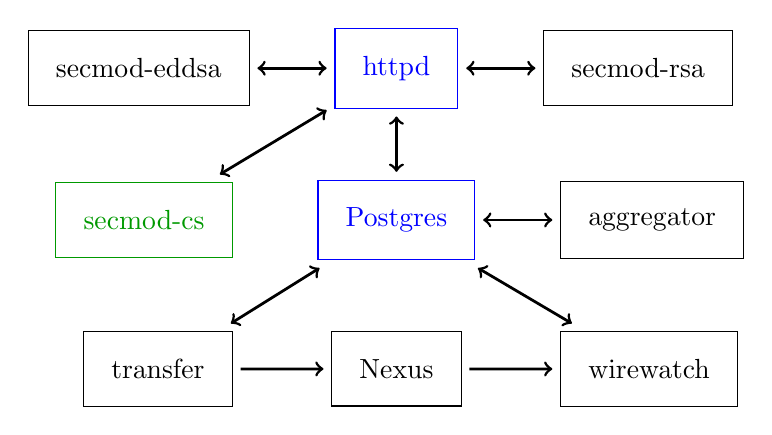
\begin{tikzpicture}
      \tikzstyle{def} = [node distance=2em and 2.5em, inner sep=1em, outer sep=.3em];
      \node (origin) at (0,0) {};
      \node [blue] (httpd) [def,above=of origin,draw]{httpd};
      \node (secmod-rsa) [def, draw, right=of httpd] {secmod-rsa};
      \node (secmod-eddsa) [def, draw, left=of httpd] {secmod-eddsa};
      \node [blue](postgres) [def, draw, below=of httpd]{Postgres};
      \node [mGreen] (secmod-cs) [def, draw, left=of postgres]{secmod-cs};
      \node (aggregator) [def, draw, right=of postgres]{aggregator};
      \node (transfer) [def, draw, below left=of postgres]{transfer};
      \node (wirewatch) [def, draw, below right=of postgres]{wirewatch};
      \node (nexus) [def, draw, below=of postgres]{Nexus};

      \tikzstyle{C} = [color=black, line width=1pt]

      \draw [<->, C] (httpd) -- (postgres) node [midway, above, sloped] (TextNode) {};
      \draw [<->, C] (httpd) -- (secmod-rsa) node [midway, above, sloped] (TextNode) {};
      \draw [<->, C] (httpd) -- (secmod-eddsa) node [midway, above, sloped] (TextNode) {};
      \draw [<->, C] (httpd) -- (secmod-cs) node [midway, above, sloped] (TextNode) {};
      \draw [<->, C] (aggregator) -- (postgres) node [midway, above, sloped] (TextNode) {};
      \draw [<->, C] (wirewatch) -- (postgres) node [midway, above, sloped] (TextNode) {};
      \draw [<->, C] (transfer) -- (postgres) node [midway, above, sloped] (TextNode) {};
      \draw [->, C] (transfer) -- (nexus) node [midway, above, sloped] (TextNode) {};
      \draw [<-, C] (wirewatch) -- (nexus) node [midway, above, sloped] (TextNode) {};
    \end{tikzpicture}
  \end{center}
  \caption{Taler exchange architecture (source: \cite{taler-presentation})}
  \label{fig:taler:exchange-architecture}
\end{figure}

\subsection{Wallet}
The architecture of the wallet implementation (as seen in figure \ref{fig:taler:wallet-architecture}) is quite straightforward.
To add support for \gls{CSBS} in the wallet, the cryptographic routines need to be reimplemented in Typescript.
Taler uses tweetnacl \cite{bern:tweetnacl} which provides functionality for the group operations.
There are existing \gls{hkdf} and \gls{fdh} implementations, that can be reused.\\
Furthermore, the Taler protocols need to be adjusted to support \gls{CSBS} in the wallet-core.

\begin{figure}[h!]
  \begin{center}
    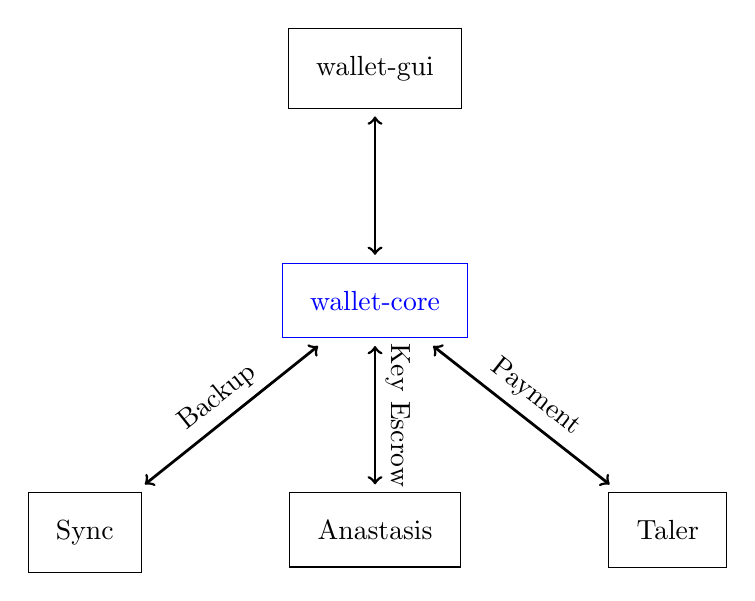
\begin{tikzpicture}
      \tikzstyle{def} = [node distance= 5em and 4.5em, inner sep=1em, outer sep=.3em];
      \node (origin) at (0,0) {};
      \node (gui) [def,above=of origin,draw]{wallet-gui};
      \node [blue](core) [def,below=of gui,draw]{wallet-core};
      \node (sync) [def, draw, below left=of core] {Sync};
      \node (taler) [def, draw, below right=of core] {Taler};
      \node (anastasis) [def, draw, below=of core] {Anastasis};

      \tikzstyle{C} = [color=black, line width=1pt]
      \draw [<->, C] (gui) -- (core) node [midway, above, sloped] (TextNode) {};
      \draw [<->, C] (core) -- (sync) node [midway, above, sloped] (TextNode) {Backup};
      \draw [<->, C] (core) -- (taler) node [midway, above, sloped] (TextNode) {Payment};
      \draw [<->, C] (core) -- (anastasis) node [midway, above, sloped] (TextNode) {Key Escrow};
    \end{tikzpicture}
  \end{center}
  \caption{Taler wallet architecture (source: \cite{taler-presentation})}
  \label{fig:taler:wallet-architecture}
\end{figure}

\section{Persistence}
The Clause Blind Schnorr Signature scheme is quite different to \gls{RSABS}.
Despite the differences, the database model does not need to be changed.
The only change needed an additional type field, specifying whether RSA or CS is used as signature algorithm.
To persist the new structs introduced with the support for \gls{CSBS}, only the postgres helpers need to support serialization and deserialization of the new structs.

\section{Testing}
We will partially use test-driven development, meaning that we will write tests (at least for the known good case) before implementing functions, and extend them during and after development.
This allows us to check the functionality (code section, function(s)) during development, while being able to extend testing whenever we identify new test cases during development.

Test cases can be used to verify different aspects of a functionality.
These are the ones we will focus on.
\begin{itemize}
  \item \textbf{Known good}:
        Known good cases test whether a functionality works as expected.
        They are the most useful during development, because they indicate whether the code is working as expected.
  \item \textbf{Known Bad}:
        Known bad cases test whether functionality that is known not to work behaves as expected.
  \item \textbf{Determinism}:
        This case type checks whether the same input leads to the same output.
        It is important for code that must work deterministic (same output), non-deterministic (e.g. random output) or based on a state that impacts the functionality.
  \item \textbf{Performance testing}:
        Performance testing is used to gather timing information that can be used to identify functionality with long duration, or to  compare performance between different implementations or major changes.
        We will restrict performance testing to the comparison of the Blind RSA Signature Scheme and the Clause Blind Schnorr Signature Scheme.
\end{itemize}


\section{Signature Scheme Operations in GNUnet}
\label{sec:specification-signature-scheme}

The signature scheme operations implemented are needed in all other parts of the implementation.
Taler's cryptographic primitives (e.g. \gls{RSABS}, \gls{hkdf}, hash functions) are mostly implemented in GNUnet utils, therefore the Clause Blind Schnorr Signature routines will be implemented in GNUnet too.
It is important to provide a clear API for the cryptographic routines and to test them thoroughly.
Libsodium will be used for finite field arithmetic (\cite{libsodium:finite-field-arithmetic}) and for other functionality when available (e.g. for key generation).
Thus, a widely used and well tested cryptographic library is used for group operations.

For \acl{FDH} and \gls{hkdf} existing implementations provided by GNUnet are used.
The \gls{hkdf} is used with SHA-512 for the extraction phase and SHA-256 for the expansion phase.

\subsection{Data Structures}
Libsodium represents Ed25519 points and scalars as 32-byte char arrays.
To provide a more user-friendly \ac{API}, structs were created to represent each type.
For example \texttt{struct GNUNET\_CRYPTO\_CsPrivateKey} or  \texttt{struct GNUNET\_CRYPTO\_RSecret}
The main reason is to increase readability and to prevent misusage of the \ac{API}.
Unlike RSA, our \gls{CSBS} on Ed25519 data structures have a fixed sizes.
The different data structures can be found in table \ref{tab:datastruct-crypto}.

\begin{table}[ht]
  \centering
  \resizebox{0.95\textwidth}{!}{\begin{minipage}{\textwidth}
  \colorlet{BFH-table}{BFH-MediumBlue!10}
  \colorlet{BFH-tablehead}{BFH-MediumBlue!50}
  \setupBfhTabular
  \begin{tabular}{lll}
      \rowcolor{BFH-tablehead}
      \textbf{Values} & \textbf{Data Structure} & \textbf{Data Type} \\\hline
      Curve25519 Scalar & {\small GNUNET\_CRYPTO\_Cs25519Scalar} & 32 byte char array\\\hline
      Curve25519 Point & {\small GNUNET\_CRYPTO\_Cs25519Point} & 32 byte char array\\\hline
      Private Key & {\small GNUNET\_CRYPTO\_CsPrivateKey} & {\small GNUNET\_CRYPTO\_Cs25519Scalar}\\\hline
      Public Key & {\small GNUNET\_CRYPTO\_CsPublicKey} & {\small GNUNET\_CRYPTO\_Cs25519Point}\\\hline
      $\alpha, \beta$ & {\small GNUNET\_CRYPTO\_CsBlindingSecret} & {\footnotesize 2x GNUNET\_CRYPTO\_Cs25519Scalar}\\\hline
      $r$ & {\small GNUNET\_CRYPTO\_CsRSecret} & {\small GNUNET\_CRYPTO\_Cs25519Scalar}\\\hline
      $R$ & {\small GNUNET\_CRYPTO\_CsRPublic} & {\small GNUNET\_CRYPTO\_Cs25519Point}\\\hline
      $c$ & {\small GNUNET\_CRYPTO\_CsC} & {\small GNUNET\_CRYPTO\_Cs25519Scalar}\\\hline
      $s$ & {\small GNUNET\_CRYPTO\_CsBlindS} & {\small GNUNET\_CRYPTO\_Cs25519Scalar}\\\hline
      $s'$ & {\small GNUNET\_CRYPTO\_CsS} & {\small GNUNET\_CRYPTO\_Cs25519Scalar}\\\hline
      $\sigma := \langle s',R' \rangle$ & {\small GNUNET\_CRYPTO\_CsSignature} & {\small GNUNET\_CRYPTO\_Cs25519Scalar}\\
      & & {\small GNUNET\_CRYPTO\_Cs25519Point}\\\hline
      Nonce & {\small GNUNET\_CRYPTO\_CsNonce} & 32 byte char array\\\hline
  \end{tabular}
  \caption{Data structures for cryptographic routines}
  \label{tab:datastruct-crypto}
\end{minipage}}
\end{table}



\subsection{Library API}
The public \ac{API} and related data structures are specified in the C header file \url{src/include/gnunet_crypto_lib.h} in the GNUnet repository \cite{gnunet-git}.
It was developed in multiple iterations based on feedback from Christian Grothoff.
The complete C header \ac{API} can be found in the repository.
This section provides an overview of the implemented crypto API.

Some design decisions need to be explained further:
\begin{itemize}
  \item In order to prevent misusage of our implementation and increase readability, the functions that represent different stages in the signature scheme takes different data types as in- and output.
        Internally most variables are either scalars or curve points (except for nonces, secrets and messages).
  \item Operations that are performed twice in the Clause Blind Schnorr Signature Scheme (e.g. derivation of $ r $) do not have to be called twice.
        Instead, the API returns an array of two instead of a single value.\\
        For these functions, we also optimized the \gls{hkdf} (as proposed by Christian Grothoff).
        Instead of calling \gls{hkdf} twice (with different salts, e.g. "r0" and "r1"), we call it one time (e.g. with salt "r") and double the output length.
  \item The cryptographic hash function used to derive $ c' $ (hash of $ R' $ and message) must map the results into the main subgroup for scalars, meaning that it has to be a \gls{fdh} (see \ref{sec:rsa-fdh}).
\end{itemize}

The following API examples should provide an overview on how the API works and how to use it.

First of all the API must provide functionality to create a \gls{25519} keypair as in listing \ref{lst:crypto-keypair-api}

\begin{lstlisting}[style=bfh-c,language=C, caption={GNUnet create keypair API}, label={lst:crypto-keypair-api}]
/**
 * Create a new random private key.
 *
 * @param[out] priv where to write the fresh private key
 */
void
GNUNET_CRYPTO_cs_private_key_generate (
    struct GNUNET_CRYPTO_CsPrivateKey *priv);


/**
 * Extract the public key of the given private key.
 *
 * @param priv the private key
 * @param[out] pub where to write the public key
 */
void
GNUNET_CRYPTO_cs_private_key_get_public (
    const struct GNUNET_CRYPTO_CsPrivateKey *priv,
    struct GNUNET_CRYPTO_CsPublicKey *pub);
\end{lstlisting}

The signer needs an API to generate his secret $r$ and calculate his public point $R$.
As specified in the redesign of the protocols, the r must not be chosen randomly because we need to provide \textit{\gls{abort-idempotency}}. However, the secret $r$ still needs to be \textit{unpredictable} and look random to the client.
The r\_derive API derives such a secret $r$ from a nonce and a long-term secret with \gls{hkdf}.
Further, the API ensures that a caller must generate two secret $r$ as in the Clause Blind Schnorr Signature scheme. This should discourage people from using the unsecure Blind Schnorr Signature scheme. See \ref{lst:crypto-rderive-api}.


\begin{lstlisting}[style=bfh-c,language=C, caption={GNUnet r derive API}, label={lst:crypto-rderive-api}]
 /**
  * Derive a new secret r pair r0 and r1.
  * In original papers r is generated randomly
  * To provide abort-idempotency, r needs to be derived but still needs to be UNPREDICTABLE
  * To ensure unpredictability a new nonce should be used when a new r needs to be derived.
  * Uses HKDF internally.
  * Comment: Can be done in one HKDF shot and split output.
  *
  * @param nonce is a random nonce
  * @param lts is a long-term-secret in form of a private key
  * @param[out] r array containing derived secrets r0 and r1
  */
 void
 GNUNET_CRYPTO_cs_r_derive (const struct GNUNET_CRYPTO_CsNonce *nonce,
                            const struct GNUNET_CRYPTO_CsPrivateKey *lts,
                            struct GNUNET_CRYPTO_CsRSecret r[2]);


/**
  * Extract the public R of the given secret r.
  *
  * @param r_priv the private key
  * @param[out] r_pub where to write the public key
  */
 void
 GNUNET_CRYPTO_cs_r_get_public (const struct GNUNET_CRYPTO_CsRSecret *r_priv,
                                struct GNUNET_CRYPTO_CsRPublic *r_pub);
\end{lstlisting}


Same as the r\_derive, the blinding secrets are also derived and not generated randomly.
The blinding secrets are generated by a client who provides a secret as seed to derive the secrets from as in listing \ref{lst:crypto-blinding-secrets-api}.

\begin{lstlisting}[style=bfh-c,language=C, caption={GNUnet blinding secrets derive API}, label={lst:crypto-blinding-secrets-api}]
/**
 * Derives new random blinding factors.
 * In original papers blinding factors are generated randomly
 * To provide abort-idempotency, blinding factors need to be derived but still need to be UNPREDICTABLE
 * To ensure unpredictability a new nonce has to be used.
 * Uses HKDF internally
 *
 * @param secret is secret to derive blinding factors
 * @param secret_len secret length
 * @param[out] bs array containing the two derivedGNUNET_CRYPTO_CsBlindingSecret
 */
void
GNUNET_CRYPTO_cs_blinding_secrets_derive (
    const struct GNUNET_CRYPTO_CsNonce *blind_seed,
    struct GNUNET_CRYPTO_CsBlindingSecret bs[2]);
\end{lstlisting}

Further the Clause Blind Schnorr API provides an API to calculate the two blinded c of the message with the two public $R$, the blinding factors and the public key as in listing \ref{lst:crypto-calc-c-api}.

\begin{lstlisting}[style=bfh-c,language=C, caption={GNUnet calculate blinded c API}, label={lst:crypto-calc-c-api}]
/**
 * Calculate two blinded c's
 * Comment: One would be insecure due to Wagner's algorithm solving ROS
 *
 * @param bs array of the two blinding factor structs each containing alpha and beta
 * @param r_pub array of the two signer's nonce R
 * @param pub the public key of the signer
 * @param msg the message to blind in preparation for signing
 * @param msg_len length of message msg
 * @param[out] blinded_c array of the two blinded c's
 */
void
GNUNET_CRYPTO_cs_calc_blinded_c (
    const struct GNUNET_CRYPTO_CsBlindingSecret bs[2],
    const struct GNUNET_CRYPTO_CsRPublic r_pub[2],
    const struct GNUNET_CRYPTO_CsPublicKey *pub,
    const void *msg,
    size_t msg_len,
    struct GNUNET_CRYPTO_CsC blinded_c[2]);
\end{lstlisting}

The sign function in our API is called sign\_derive, since we derive $b \in \{0,1\}$ from the long-term secret and then calculate the signature scalar of $c_b$.
See listing \ref{lst:crypto-sign-api}.

\begin{lstlisting}[style=bfh-c,language=C, caption={GNUnet sign API}, label={lst:crypto-sign-api}]
/**
 * Sign a blinded c
 * This function derives b from a nonce and a longterm secret
 * In original papers b is generated randomly
 * To provide abort-idempotency, b needs to be derived but still need to be UNPREDICTABLE.
 * To ensure unpredictability a new nonce has to be used for every signature
 * HKDF is used internally for derivation
 * r0 and r1 can be derived prior by using GNUNET_CRYPTO_cs_r_derive
 *
 * @param priv private key to use for the signing and as LTS in HKDF
 * @param r array of the two secret nonce from the signer
 * @param c array of the two blinded c to sign c_b
 * @param nonce is a random nonce
 * @param[out] blinded_signature_scalar where to write the signature
 * @return 0 or 1 for b (see Clause Blind Signature Scheme)
 */
int
GNUNET_CRYPTO_cs_sign_derive(
    const struct GNUNET_CRYPTO_CsPrivateKey *priv,
    const struct GNUNET_CRYPTO_CsRSecret r[2],
    const struct GNUNET_CRYPTO_CsC c[2],
    const struct GNUNET_CRYPTO_CsNonce *nonce,
    struct GNUNET_CRYPTO_CsBlindS *blinded_signature_scalar);
\end{lstlisting}

The API for the unblind operation can be called with the blinding secrets and the signature scalar received from the signer as in listing \ref{lst:crypto-unblind-api}.

\begin{lstlisting}[style=bfh-c,language=C, caption={GNUnet unblind API}, label={lst:crypto-unblind-api}]
  /**
 * Unblind a blind-signed signature using a c that was blinded
 *
 * @param blinded_signature_scalar the signature made on the blinded c
 * @param bs the blinding factors used in the blinding
 * @param[out] signature_scalar where to write the unblinded signature
 */
void
GNUNET_CRYPTO_cs_unblind (
    const struct GNUNET_CRYPTO_CsBlindS *blinded_signature_scalar,
    const struct GNUNET_CRYPTO_CsBlindingSecret *bs,
    struct GNUNET_CRYPTO_CsS *signature_scalar);
\end{lstlisting}

The verify API takes the message and its signature with the public key and returns GNUNET\_OK for a valid signature and GNUNET\_SYSERR otherwise.
See listing \ref{lst:crypto-verify-api}.

\begin{lstlisting}[style=bfh-c,language=C,, caption={GNUnet verify API}, label={lst:crypto-verify-api}]
  /**
  * Verify whether the given message corresponds to the given signature and the
  * signature is valid with respect to the given public key.
  *
  * @param sig signature that is being validated
  * @param pub public key of the signer
  * @param msg is the message that should be signed by @a sig  (message is used to calculate c)
  * @param msg_len is the message length
  * @returns #GNUNET_YES on success, #GNUNET_SYSERR if signature invalid
  */
 enum GNUNET_GenericReturnValue
 GNUNET_CRYPTO_cs_verify (const struct GNUNET_CRYPTO_CsSignature *sig,
                          const struct GNUNET_CRYPTO_CsPublicKey *pub,
                          const void *msg,
                          size_t msg_len);
\end{lstlisting}

\subsection{Testing}
For digital signature schemes, the most important test case is the \textit{known good} case where a signature is created and successfully validated.
This test case already tests very much in a digital signature scheme.
When the signature creation or verification has a bug, a test will not succeed, because the mathematic operations need to be correct to be validated correctly.

The cryptographic operations are further tested for deterministicy (where it applies), meaning that multiple function calls with the same input must lead to the same output.

Since libsodium is used for the finite field arithmetic operations and is a well tested library, many cryptographic tests are already done in libsodium.

The performance is measured in a benchmark to see how performant \gls{CSBS} are in comparison to the RSA Blind Signature Scheme.

\section{Taler Cryptographic Utilities}
Taler provides utility functions to support cryptographic operations.\\
This chapter provides an overview of these utility functions and about the functionality they provide.

\subsection{Planchet Creation}
In crypto.c many utility functions are provided to create planchets (for planchet details see \ref{fig:coin:states}), blinding secrets and much more.
One difference between \gls{RSABS} and \gls{CSBS} is, that the coin private key and RSA blinding secret can be created at the same point in time, since the RSA blinding secret is created randomly.
However, for Clause Blind Schnorr secrets an additional step is needed, the public $R_0$ and $R_1$ are required to calculate the blinding seed to derive the secrets.

A planchet in the Clause Blind Schnorr Signature Scheme can be created as followed (implementation details omitted).

\begin{enumerate}
  \item Create planchet with new \ac{EdDSA} private key
  \item Derive withdraw nonce
  \item Request public $R_0, R_1$ from signer
  \item Derive blinding seed
  \item Prepare (blind) the planchet
\end{enumerate}

After the planchet is created, it is sent to the exchange to be signed.

\subsection{Taler CS Security Module}
The exchange segregates access to the private keys with separate security module processes.
The security module has sole access to the private keys of the online signing keys and thus, only a security module can create signatures.
The different \textit{taler-exchange-secmod} processes (separated by signature scheme) are managing the exchanges online signing keys. The RSA denomination keys for example are managed with \textit{taler-exchange-secmod-rsa}.

Now a new \textit{taler-exchange-secmod-cs} needs to be created for managing the \gls{CSBS} denomination keys.
These security modules run on the same machine as the httpd process and they use UNIX Domain Sockets as method for \acl{IPC}.
A short introduction about UNIX Domain Sockets can be found in the blog post \cite{matt:unix-domain-sockets}.
Furthermore, the security modules are used to protect the online signing keys by performing the actual signing operations in the dedicated taler-secmod-cs process.
This abstraction makes it harder for an attacker who has already compromised the http daemon to gain access to the private keys.
However, such an attacker would still be able to sign arbitrary messages (see \cite{taler-documentation:exchange-operator-manual}).
A crypto helper exists for each security module, these functions can be called inside the exchange for operations requiring the private online signing keys.
The new Clause Schnorr security module and corresponding crypto helper provides the following functionality:
\begin{itemize}
  \item Private Key Management and creation
  \item Request public $R_0, R_1$
  \item Request a signature of a $c_0,c_1$ pair
  \item Revoke an online signing key
\end{itemize}

\subsection{Testing}
All of the operations have tests and are included in unit tests.
As a template for testing, the existing RSA tests were used and adjusted for \gls{CSBS}.


\section{Denomination Key Management}
Since we introduce a type of denomination keys, related operations like connection to the \gls{CSBS} security module, making the denominations available for customers, persisting them in the database and offline signing using the exchange's offline signature key have to be extended to incorporate the \acl{CS}.

The exchange offline signer requests the future, not yet signed keys by calling GET \url{/management/keys} as described in table \ref{tab:management-keys-get}. \\\\
\framebox[1.1\width]{\color{blue}\texttt{GET /management/keys}}
\begin{table}[ht]
  \centering
  \resizebox{0.9\textwidth}{!}{\begin{minipage}{\textwidth}
  \colorlet{BFH-table}{BFH-MediumBlue!10}
  \colorlet{BFH-tablehead}{BFH-MediumBlue!50}
  \setupBfhTabular
  \begin{tabular}{ll}
      \rowcolor{BFH-tablehead}
      \textbf{Field} & \textbf{Value} \\
      future\_denoms & Information about denomination keys \\
      future\_signkeys & Information about exchange online signing keys \\
      master\_pub & Exchange's master public key \\
      denom\_secmod\_public\_key & RSA security module public key \\
      denom\_secmod\_cs\_public\_key & \gls{CSBS} security module public key \\
      signkey\_secmod\_public\_key & Online singing security module public key \\
  \end{tabular}
  \caption{GET \url{/management/keys} response data}
  \label{tab:management-keys-get}
\end{minipage}}
\end{table}

It then signs the keys and returns them using POST on the same \ac{URL} with the data described in table  \ref{tab:management-keys-post}. \\\\
\framebox[1.1\width]{\color{blue}\texttt{POST /management/keys}}
\begin{table}[ht]
  \centering
  \colorlet{BFH-table}{BFH-MediumBlue!10}
  \colorlet{BFH-tablehead}{BFH-MediumBlue!50}
  \setupBfhTabular
  \begin{tabular}{ll}
      \rowcolor{BFH-tablehead}
      \textbf{Field} & \textbf{Value} \\
      denom\_sigs & Denomination key signatures \\
      signkey\_sigs & Online signing key signatures \\
  \end{tabular}
  \caption{POST \url{/management/keys} response data}
  \label{tab:management-keys-post}
\end{table}

Wallets can then call GET \url{/keys} to obtain the current denominations and other information, the response is described in table \ref{tab:keys-get}. \\\\
\framebox[1.1\width]{\color{blue}\texttt{GET /keys}}
\begin{table}[ht]
  \centering
  \colorlet{BFH-table}{BFH-MediumBlue!10}
  \colorlet{BFH-tablehead}{BFH-MediumBlue!50}
  \setupBfhTabular
  \begin{tabular}{ll}
      \rowcolor{BFH-tablehead}
      \textbf{Field} & \textbf{Value} \\
      version & Exchange's protocol version \\
      currency & Currency \\
      master\_public\_key & Exchange's master public key \\
      reserve\_closing\_delay & Delay before reserves are closed \\
      signkeys & Exchange's online signing public keys \\
      recoup & Revoked keys \\
      denoms & List of denominations \\
      auditors & Auditors for this exchange \\
      list\_issue\_date & Timestamp \\
      eddsa\_pub & Exchange's online signing public key \\
      eddsa\_sig & Signature (use "eddsa\_pub" for verification) \\
  \end{tabular}
  \caption{GET \url{/keys} response data}
  \label{tab:keys-get}
\end{table}


\section{New Endpoint for $R$}
The withdraw and refresh protocols using the  Claude Blind Schnorr Signature Scheme introduce an additional round trip.
In this round trip, the customer requests two $ R $ from the exchange.
The exchange uses a secret $ r $ to calculate $ R := rG $.
\\
In contrast to the plain Clause Blind Schnorr Signature Scheme (see \ref{sec:clause-blind-schnorr-sig}), $ r $ isn't generated randomly but instead derived using a \gls{hkdf} with a nonce from the customer and a denomination private key (secret only known by the exchange).
This still ensures that the private $ r $ can't be anticipated, but has multiple advantages regarding \gls{abort-idempotency}.
\Gls{abort-idempotency} means that a withdraw or refresh operation can be aborted in any step and later tried again (using the same values) without yielding a different result.
The challenge for $ r, R $ regarding \gls{abort-idempotency} is to ensure that the same $ r $ is used during the complete signature creation process.

The only drawback of this process is that we have to ensure that the same nonce and secret aren't used for different withdraw- or refresh-operations.
This is done during signature creation and will be described in the withdraw protocol section \ref{sec:specification-withdraw}.


\subsection{Public APIs and Data Structures}
This is a new functionality, meaning a new endpoint accessible to customers has to be introduced.
It will be made available in the exchange HTTP server under \framebox[1.1\width]{\color{blue}\texttt{POST /csr}} and will take the input parameters described in table \ref{tab:csr-request-data} (as \ac{JSON}).
\begin{table}[ht]
  \centering
  \resizebox{0.9\textwidth}{!}{\begin{minipage}{\textwidth}
  \colorlet{BFH-table}{BFH-MediumBlue!10}
  \colorlet{BFH-tablehead}{BFH-MediumBlue!50}
  \setupBfhTabular
  \begin{tabular}{lll}
      \rowcolor{BFH-tablehead}
      \textbf{Field} & \textbf{Type} & \textbf{Value} \\
      nonce & String & 32 Bytes encoded in Crockford base32 Hex \\
      denom\_pub\_hash & String & Denomination Public Key encoded in Crockford base32 Hex \\
  \end{tabular}
  \caption{POST \url{/csr} request data}
  \label{tab:csr-request-data}
\end{minipage}}
\end{table}

The exchange will then check the denomination and return one of these HTTP status codes:
\begin{itemize}
  \item \textbf{200 (HTTP\_OK)}: Request Successful
  \item \textbf{400 (BAD\_REQUEST)}: Invalid input parameters
  \item \textbf{404 (NOT\_FOUND)}: Denomination unknown or not Clause Schnorr
  \item \textbf{410 (GONE)}: Denomination revoked/expired
  \item \textbf{412 (PRECONDITION\_FAILED)}: Denomination not yet valid
\end{itemize}

When the request was successful, the exchange returns the data described in table \ref{tab:csr-response-data} (as \ac{JSON}).
\begin{table}[ht]
  \centering
  \colorlet{BFH-table}{BFH-MediumBlue!10}
  \colorlet{BFH-tablehead}{BFH-MediumBlue!50}
  \setupBfhTabular
  \begin{tabular}{lll}
      \rowcolor{BFH-tablehead}
      \textbf{Field} & \textbf{Type} & \textbf{Value} \\
      r\_pub\_0 & String & 32 Bytes encoded in Crockford base32 Hex \\
      r\_pub\_1 & String & 32 Bytes encoded in Crockford base32 Hex \\
  \end{tabular}
  \caption{POST \url{/csr} response data}
  \label{tab:csr-response-data}
\end{table}


\subsection{Persistence}
This API does not persist anything.
This is because the resulting $R_0, R_1$ are derived and can be derived in a later step.


\section{Withdraw Protocol}
\label{sec:specification-withdraw}
The withdraw protocol has been introduced in section \ref{sec:withdrawal}.
For the \acl{CS} necessary adjustments are described in section \ref{sec:withdraw-protocol-schnorr}.


\subsection{Public APIs and Data Structures}
\label{sec:specification-withdraw-public-api}
The existing endpoint is available under \texttt{POST /reserves/[reserve]/withdraw} where "reserve" is the reserve public key encoded as Crockford base32.
It takes the following input parameters described in table \ref{tab:withdraw-request-data} as JSON.\\\\
\framebox[1.1\width]{\color{blue}\texttt{POST /reserves/[reserve]/withdraw}}
\begin{table}[ht]
  \centering
  \colorlet{BFH-table}{BFH-MediumBlue!10}
  \colorlet{BFH-tablehead}{BFH-MediumBlue!50}
  \setupBfhTabular
  \begin{tabular}{ll}
      \rowcolor{BFH-tablehead}
      \textbf{Field} & \textbf{Value} \\
      denom\_pub\_hash & Denomination Public Key \\
      coin\_ev & RSA blinded coin public key \\
      reserve\_sig & Signature over the request using the reserve's private key \\
  \end{tabular}
  \caption{Withdraw request data}
  \label{tab:withdraw-request-data}
\end{table}

In order to facilitate parsing, Christian Grothoff suggested to include the cipher type in the "coin\_ev" field, thus creating a nested \ac{JSON} (as described in table \ref{tab:withdraw-coin-ev-rsa}).
\begin{table}[ht]
  \centering
  \colorlet{BFH-table}{BFH-MediumBlue!10}
  \colorlet{BFH-tablehead}{BFH-MediumBlue!50}
  \setupBfhTabular
  \begin{tabular}{lll}
      \rowcolor{BFH-tablehead}
      \textbf{Field} & \textbf{Type} & \textbf{Value} \\
      cipher & Integer & Denomination cipher: 1 stands for RSA \\
      rsa\_blinded\_planchet & String & RSA blinded coin public key \\
  \end{tabular}
  \caption{Withdraw "coin\_ev" field (RSA)}
  \label{tab:withdraw-coin-ev-rsa}
\end{table}

For the Clause Schnorr implementation, the field "rsa\_blinded\_planchet" will be replaced with the necessary values as described in table \ref{tab:withdraw-coin-ev-cs}.
\begin{table}[ht]
  \centering
  \resizebox{0.85\textwidth}{!}{\begin{minipage}{\textwidth}
  \colorlet{BFH-table}{BFH-MediumBlue!10}
  \colorlet{BFH-tablehead}{BFH-MediumBlue!50}
  \setupBfhTabular
  \begin{tabular}{lll}
    \rowcolor{BFH-tablehead}
    \textbf{Field} & \textbf{Type} & \textbf{Value} \\
    cipher & Integer & Denomination cipher: 2 stands for \gls{CSBS} \\
    cs\_nonce & String & 32 Bytes encoded in Crockford base32 Hex \\
    cs\_blinded\_c0 & String & 32 Bytes encoded in Crockford base32 Hex \\
    cs\_blinded\_c1 & String & 32 Bytes encoded in Crockford base32 Hex \\
  \end{tabular}
  \caption{Withdraw "coin\_ev" field (\gls{CSBS})}
  \label{tab:withdraw-coin-ev-cs}
\end{minipage}}
\end{table}

The exchange will then process the withdraw request and return one of these HTTP status codes:
\begin{itemize}
  \item \textbf{200 (HTTP\_OK)}: Request Successful
  \item \textbf{400 (BAD\_REQUEST)}: Invalid input parameters (can also happen if denomination cipher doesn't match with cipher in "coin\_ev")
  \item \textbf{403 (FORBIDDEN)}: Signature contained in "reserve\_sig" invalid
  \item \textbf{404 (NOT\_FOUND)}: Denomination unknown
  \item \textbf{410 (GONE)}: Denomination revoked/expired
  \item \textbf{412 (PRECONDITION\_FAILED)}: Denomination not yet valid
\end{itemize}

When the request was successful, the exchange returns the RSA signature as JSON (described in table \ref{tab:withdraw-response-rsa}).
\begin{table}[ht]
  \centering
  \colorlet{BFH-table}{BFH-MediumBlue!10}
  \colorlet{BFH-tablehead}{BFH-MediumBlue!50}
  \setupBfhTabular
  \begin{tabular}{lll}
      \rowcolor{BFH-tablehead}
      \textbf{Field} & \textbf{Type} & \textbf{Value} \\
      cipher & Integer & Denomination cipher: 1 stands for RSA \\
      blinded\_rsa\_signature & String & RSA signature \\
  \end{tabular}
  \caption{Withdraw response (RSA)}
  \label{tab:withdraw-response-rsa}
\end{table}

Table \ref{tab:withdraw-response-cs} describes the response for \gls{CSBS}.
\begin{table}[ht]
  \centering
  \resizebox{0.85\textwidth}{!}{\begin{minipage}{\textwidth}
  \colorlet{BFH-table}{BFH-MediumBlue!10}
  \colorlet{BFH-tablehead}{BFH-MediumBlue!50}
  \setupBfhTabular
  \begin{tabular}{lll}
      \rowcolor{BFH-tablehead}
      \textbf{Field} & \textbf{Type} & \textbf{Value} \\
      cipher & Integer & Denomination cipher: 2 stands for \gls{CSBS} \\
      b & Integer & \gls{CSBS} signature session identifier (either 0 or 1) \\
      s & String & signature scalar (32 Bytes encoded in Crockford base32 Hex) \\
  \end{tabular}
  \caption{Withdraw response (\gls{CSBS})}
  \label{tab:withdraw-response-cs}
\end{minipage}}
\end{table}


\subsection{Persistence}
Persistence for withdrawing is implemented in the function \texttt{postgres\_do\_withdraw} in \texttt{src/exchangedb/plugin\_exchangedb\_postgres.c}
For \gls{CSBS}, persisting the blinded signature must be implemented.


\section{Deposit Protocol}
For the deposit protocol (described in section \ref{sec:deposit-protocol}) only the handling and verification of \gls{CSBS} signatures has to be added.

\subsection{Public APIs and Data Structures}
Deposit is an existing endpoint available under \texttt{POST /coins/[coin public key]/deposit} where "coin public key" is encoded as Crockford base32.
Additional parameters are passed as JSON (as described in table \ref{tab:spend-request}).\\\\
\framebox[1.1\width]{\color{blue}\texttt{POST /coins/[coin public key]/deposit}}
\begin{table}[ht]
  \centering
  \colorlet{BFH-table}{BFH-MediumBlue!10}
  \colorlet{BFH-tablehead}{BFH-MediumBlue!50}
  \setupBfhTabular
  \begin{tabular}{ll}
      \rowcolor{BFH-tablehead}
      \textbf{Field} & \textbf{Value} \\
      % cipher & Denomination cipher: 2 stands for \gls{CSBS} \\
      % b & \gls{CSBS} signature session identifier (either 0 or 1) \\
      % s & signature scalar (32 Bytes encoded in Crockford base32 Hex) \\
      merchant\_payto\_uri & Account that is credited  \\
      wire\_salt & Salt used by the merchant \\
      contribution & Amount to use for payment (for one specific coin) \\
      denom\_pub\_hash & Denomination public key hash \\
      ub\_sig & (unblinded) denomination signature of coin \\
      merchant\_pub & Merchant public key \\
      h\_contract\_terms & Contract terms hash \\
      coin\_sig & Deposit permission signature \\
      timestamp & Timestamp of generation \\
      refund\_deadline (optional) & Refund deadline \\
      wire\_transfer\_deadline (optional) & Wire transfer deadline \\
  \end{tabular}
  \caption{Spend request}
  \label{tab:spend-request}
\end{table}

Relevant field for the \gls{CSBS} implementation is the field "ub\_sig" containing the unblinded denomination signature of the coin.
For RSA, the (nested) \ac{JSON} is described in table \ref{tab:spend-request-ubsig-rsa}.
\begin{table}[ht]
  \centering
  \colorlet{BFH-table}{BFH-MediumBlue!10}
  \colorlet{BFH-tablehead}{BFH-MediumBlue!50}
  \setupBfhTabular
  \begin{tabular}{lll}
      \rowcolor{BFH-tablehead}
      \textbf{Field} & \textbf{Type} & \textbf{Value} \\
      cipher & Integer & Denomination cipher: 1 stands for RSA \\
      rsa\_signature & String & Unblinded RSA signature \\
  \end{tabular}
  \caption{ub\_sig (RSA)}
  \label{tab:spend-request-ubsig-rsa}
\end{table}

Table \ref{tab:spend-request-ubsig-cs} describes the values in "ub\_sig" required for \gls{CSBS}.
\begin{table}[ht]
  \centering
  \resizebox{0.85\textwidth}{!}{\begin{minipage}{\textwidth}
  \colorlet{BFH-table}{BFH-MediumBlue!10}
  \colorlet{BFH-tablehead}{BFH-MediumBlue!50}
  \setupBfhTabular
  \begin{tabular}{lll}
      \rowcolor{BFH-tablehead}
      \textbf{Field} & \textbf{Type} & \textbf{Value} \\
      cipher & Integer & Denomination cipher: 2 stands for \gls{CSBS} \\
      cs\_signature\_r & String & Curve point $ R' $ (32 Bytes encoded in Crockford base32 Hex) \\
      cs\_signature\_s & String & Signature scalar (32 Bytes encoded in Crockford base32 Hex) \\
  \end{tabular}
  \caption{ub\_sig (\gls{CSBS})}
  \label{tab:spend-request-ubsig-cs}
\end{minipage}}
\end{table}


\subsection{Persistence}
Persistence is handled in the functions \texttt{postgres\_insert\_deposit} and\\ \texttt{postgres\_have\_deposit} located in \url{src/exchangedb/plugin_exchangedb_postgres.c}.
However, these functions are not containing \gls{CSBS}-specific persistence.
\\What needs to be adjusted however, is the function \texttt{postgres\_ensure\_coin\_known} called by the function \texttt{TEH\_make\_coin\_known} (located in \url{src/exchange/taler-exchange-httpd_db.c}).


% \section{Tipping}
% \subsection{Public APIs and Data Structures}
% \subsection{Code Location}
% \subsection{Persistence}
% \subsection{Used Libraries}

% \section{Payback Protocol}
% \subsection{Public APIs and Data Structures}
% \subsection{Code Location}
% \subsection{Persistence}
% \subsection{Used Libraries}


% sollte ein Product Backlog das Ziel dieser Phase sein?


\chapter{Implementation}
\label{chap:implement}
This chapter gives an overview on the implementation challenges and discusses special parts in the implementation.


\section{Signature Scheme Operations}
The signature scheme operations are implemented in the GNUnet core repository \cite{gnunet-git} (and have been merged into the master branch).
This would allow other GNUnet projects to use our implementation of the Clause Blind Schnorr Signature Scheme.

The implementation is done in multiple locations:
\begin{itemize}
  \item \texttt{src/include/gnunet\_crypto\_lib.h}:
        This header file is included when using GNUnet's cryptography implementation.
  \item \texttt{src/util/crypto\_cs.c}:
        The functions specified in \texttt{gnunet\_crypto\_lib.h} will be implemented here.
  \item \texttt{src/util/test\_crypto\_cs.c}:
        The test cases for the signature scheme will be implemented here.
  \item \texttt{src/util/perf\_crypto\_cs.c}:
        This file houses the implementation of a small program that will be used to compare the performance against the blind RSA Signature Scheme.
\end{itemize}

The specification explaining the \ac{API} can be found in section \ref{sec:specification-signature-scheme}. There are two internal functions that have to be explained further in this section.

The \texttt{map\_to\_scalar\_subgroup} function clamps scalars, which is necessary for values that are derived using a \gls{hkdf}.
It sets the three least significant bits to zero (making the scalar a multiple of 8), sets the most significant bit to zero and the second-most significant bit to one.
This process is further described in \cite{rfc7748} and \cite{madden:curve25519-clamping}.

\begin{lstlisting}[style=bfh-c, language=C, caption={Function map\_to\_scalar\_subgroup - Crypto API}, label={lst:map-to-scalar}]
static void
map_to_scalar_subgroup (struct GNUNET_CRYPTO_Cs25519Scalar *scalar)
{
    scalar->d[0] &= 248;
    scalar->d[31] &= 127;
    scalar->d[31] |= 64;
}
\end{lstlisting}

Another important function is the \gls{fdh} (see \ref{sec:schnorr-sig}) used to map the message to a scalar.
GNUnet provides a \gls{fdh} function, which expects libgcrypt's multi precision format.
A conversion function is provided by GNUnet, which requires the data to be in big endian format.
Since libsodium uses a little endian representation, the conversion process must include endianness conversion.
The complete \gls{fdh} including the required conversions is implemented in the function described in listing \ref{lst:cs-fdh}.
\begin{lstlisting}[style=bfh-c, language=C, caption={Function cs\_full\_domain\_hash - Crypto API}, label={lst:cs-fdh}]
static void
cs_full_domain_hash (const struct GNUNET_CRYPTO_CsRPublic *r_dash,
                     const void *msg,
                     size_t msg_len,
                     const struct GNUNET_CRYPTO_CsPublicKey *pub,
                     struct GNUNET_CRYPTO_CsC *c)
{
    ...
\end{lstlisting}

Last but not least, the implementation has one notable performance improvement not mentioned in the redesigned protocols.
In various steps \gls{hkdf} is used multiple times in a row.
For example to derive the four blinding secrets $\alpha_0, \alpha_1, \beta_0, \beta_1$.
The derivation can be done in one \gls{hkdf} call with bigger output size, 128 bit in this case.
The output then can be split in four parts and then mapped to the ed25519 subgroup.
This can be done secure, because as explained in \autoref{sec:kdf} a \gls{hkdf} output is truly random.


\section{Taler Cryptographic Utilities}
\begin{bfhNoteBox}
    Implementation is done in Taler's exchange.
    From here on the implementation can be found in the exchange git repository \cite{taler-git:exchange}.
\end{bfhNoteBox}
The cryptographic utilities of Taler can be found in \texttt{src/util}.


The implementation is done in various locations:
\begin{itemize}
    \item \texttt{src/include/taler\_crypto\_lib.h}: This header file is included when using Taler's cryptography implementation.
    The different data structures and functionality are defined here.
    \item \texttt{src/util/denom.c}: Implement denomination utility functions for \gls{CSBS} cases
    \item \texttt{src/util/crypto.c}: Adjust all utility functions to support \gls{CSBS}.
    crypto.c contains many cryptographic utility functions, for example to create planchets or blinding factors.
    \item \texttt{src/util/test\_crypto.c}: Functionality tests for crypto.c and denom.c
    \item \texttt{src/include/taler\_signatures.h}: In this header file message formats and signature constants are defined (not modified)
    \item \texttt{src/util/secmod\_signatures.c}: Utility functions for Taler security module signatures
\end{itemize}

The security module \texttt{taler-secmod-cs} is implemented here:
\begin{itemize}
    \item \texttt{src/util/taler-exchange-secmod-cs.c}: Standalone process to perform private key Clause Blind Schnorr signature operations.
    \item \texttt{src/util/taler-exchange-secmod-cs.h}: Specification of \ac{IPC} messages for the CS secmod process
    \item \texttt{src/util/taler-exchange-secmod-cs.conf}: Configuration file for the secmod process
    \item \texttt{src/util/secmod\_common.c} and \texttt{src/util/secmod\_common.h}: Common functions for the exchange's security modules (not modified)
\end{itemize}

The corresponding crypto helper, that talks with the security module, and its tests \& benchmarks are implemented here:
\begin{itemize}
    \item \texttt{src/util/crypto\_helper\_cs.c}: Utility functions to communicate with the security module
    \item \texttt{src/util/crypto\_helper\_common.c}: and \texttt{crypto\_helper\_common.h}: Common functions for the exchange security modules (not modified)
    \item \texttt{src/util/test\_helper\_cs.c}: Tests and benchmarks for the \gls{CSBS} crypto helper
\end{itemize}
% Crypto API offene Punkte:
%Input-validation of points and scalars:
% describe clamping: https://neilmadden.blog/2020/05/28/whats-the-curve25519-clamping-all-about/
% Testing: inverse operations, blinded signature test


\section{Denomination Key Management}
For the implementation, the \gls{CSBS} security module had to be connected to the key handling and the \gls{CSBS} denominations had to be integrated:
\begin{itemize}
    \item \url{src/exchange/taler-exchange-httpd_keys.h} and \\
    \url{src/exchange/taler-exchange-httpd_keys.c}: Integrate \gls{CSBS} secmod and denomination key management
    \item \url{src/exchange-tools/taler-exchange-offline.c}: Implement \gls{CSBS} case for offline signing of denomination keys
    \item \url{src/include/taler_exchange_service.h}: \\
    Add \gls{CSBS} secmod public key to struct\\TALER\_EXCHANGE\_FutureKeys
    \item \url{src/json/json_helper.c}: Implement CS case in function parse\_denom\_pub (used in taler-exchange-offline.c)
    \item \url{src/json/json_pack.c}: Implement \gls{CSBS} case in function TALER\_JSON\_pack\_denom\_pub (used in taler-exchange-httpd\_keys.c)
    \item \url{src/pq/pq_query_helper.c}: Implement \gls{CSBS} case in function qconv\_denom\_pub
    \item \url{src/pq/pq_result_helper.c}: Implement \gls{CSBS} case in function extract\_denom\_pub
\end{itemize}

In order for the tests to pass, the following changes had to be implemented:
\begin{itemize}
    \item \url{src/lib/exchange_api_management_get_keys.c}: Add denom\_secmod\_cs\_public\_key JSON parsing, implement \gls{CSBS} case \\in function TALER\_EXCHANGE\_ManagementGetKeysHandle
    \item \url{src/testing/.gitignore}: Add paths where \gls{CSBS} keys are stored (secmod-helper)
    \item \url{src/testing/test_auditor_api.conf}: Add section taler-exchange-secmod-cs
    \item \url{src/testing/test_exchange_api_keys_cherry_picking.conf}: Add section taler-exchange-secmod-cs
    \item \url{src/testing/testing_api_helpers_exchange.c}: Add \gls{CSBS} secmod start and stop logic
\end{itemize}


\section{New Endpoint for $R$}
The new endpoint is available in the exchange's HTTP server under \url{/csr}.
It parses and checks the input, passes the request for derivation of the two $ R $'s down to the \gls{CSBS} security module and returns them to the requestor.
The implementation can be found in:
\begin{itemize}
    \item \url{src/exchange/taler-exchange-httpd.c}:
    Definition for the new endpoint, calls the function that handles \url{/csr} requests
    \item \url{src/exchange/taler-exchange-httpd_responses.h} and \\
    \url{src/exchange/taler-exchange-httpd_responses.c}: \\
    Added function TEH\_RESPONSE\_reply\_invalid\_denom\_cipher\_for\_operation that indicates a failure when the endpoint is called for a non-\gls{CSBS} denomination
    \item \url{src/exchange/taler-exchange-httpd_csr.h} and \\
    \url{src/exchange/taler-exchange-httpd_csr.c}: \\
    Implementation of the request handler for the new endpoint
    \item \url{src/exchange/taler-exchange-httpd_keys.h} and \\
    \url{src/exchange/taler-exchange-httpd_keys.c}: \\
    Additional function TEH\_keys\_denomination\_cs\_r\_pub that passes down the request to derive the $ R $ to the taler-exchange-secmod-cs helper
\end{itemize}

The tests that check the functionality of the procotols are defined in \url{src/testing/} and use code that calls the \ac{API} (located in \url{src/lib/}).
Since the new endpoint is used during withdrawing coins, testing for the \url{/csr} endpoint is integrated in these protocol tests.
Therefore, a call to the endpoint was implemented and later integrated into the calls to the withdraw-\ac{API}.
Code for calling the endpoint is located in these files:
\begin{itemize}
    \item \url{src/include/taler_exchange_service.h}: \\
    Header describing functions and data structures used in withdraw and refresh testing:
    \begin{itemize}
        \item struct TALER\_EXCHANGE\_CsRHandle: Handle containing request information
        \item struct TALER\_EXCHANGE\_CsRResponse: Response details
        \item function TALER\_EXCHANGE\_CsRCallback: Callback function to deliver the results (used in withdraw and refresh)
        \item function TALER\_EXCHANGE\_csr: Used to call endpoint
        \item function TALER\_EXCHANGE\_csr\_cancel: Used to free dynamically allocated resources
    \end{itemize}
    \item \url{src/lib/exchange_api_csr.c}: Implementation of \url{/csr} request
\end{itemize}


\section{Withdraw Protocol}
\label{sec:withdraw-protocol-impl}
Since this is an existing endpoint, it was adjusted to support \gls{CSBS}.
Mainly, the in- and output-handling had to be adjusted as described in section \ref{sec:specification-withdraw-public-api}, additional cipher checks for the denomination were added and the \gls{CSBS} for persisting the request in the database was implemented.
\\\\
An interesting part of the implementation is the check whether a nonce was already used for this denomination or not (step: $s \leftarrow \text{GetWithdraw}(n_w, D_p)$).
This step ensures that the same signature will always be returned for a certain nonce.
Using the same nonce for the same denomination twice without this check would lead to the same random value $r$.
This is due to derivation of $r := \text{HKDF}(256,n_w || d_s, \text{"r"})$.
An attacker could then immediately recover the secret key by the following equation: $(h' - h) * x \mod q = s -s' \mod q$ \cite{tibouchi:attacks-schnorr-nonce}.
There are popular examples of this vulnerability in Sony Playstation 3's or Bitcoins ECDSA implementation \cite{buchanan:ps3-ecdsa-vuln} \cite{wang:bitcoin-ecdsa-vuln}.
More details on how such a vulnerability can be exploited can be found in one of the author's blog posts \cite{gian:nonce-sense}.\\
The designed Taler protocols using \gls{CSBS} are preventing this attack by checking the nonce and return the previously generated signature.
Additionally the denomination's public key is included in this check to prevent another issue explained in section \ref{sec:taler-vuln}.\\
The check is implemented by persisting a hash value over $n_w$ and $D_p$.
On every withdrawal \texttt{check\_request\_idempotent()} is called, which checks whether the persisted hash matches with the current $n_w, D_p$ pair.


\begin{itemize}
    \item \url{src/exchange/taler-exchange-httpd_withdraw.c}: Implementation of \gls{CSBS} case for withdraw endpoint
    \item \url{src/exchange/taler-exchange-httpd_keys.c}: Implement \gls{CSBS} case in function \\
    TEH\_keys\_denomination\_sign (passes the signature creation down to the crypto helpers)
    \item \url{src/include/taler_json_lib.h} and \url{src/json/json_helper.c}: \\
    Add function TALER\_JSON\_spec\_blinded\_planchet
    \item \url{src/json/json_pack.c}: \\
    Implement \gls{CSBS} case in function\\ TALER\_JSON\_pack\_blinded\_denom\_sig
    \item \url{src/pq/pq_query_helper.c}: implement \gls{CSBS} case in functions qconv\_denom\_sig and qconv\_blinded\_denom\_sig
    \item \url{src/pq/pq_result_helper.c}: Implement \gls{CSBS} case in function extract\_blinded\_denom\_sig
\end{itemize}

For testing, the \gls{CSBS}-related data structures and procedures as well as the request to the additional endpoint \url{/csr} (before performing the actual withdrawal) were integrated:
\begin{itemize}
    \item \url{src/testing/test_exchange_api.c}: Add additional tests for \gls{CSBS} withdraw
    \item \url{src/include/taler_testing_lib.h}: Specification for functions \\
    TALER\_TESTING\_cmd\_withdraw\_cs\_amount and \\
    TALER\_TESTING\_cmd\_withdraw\_cs\_amount\_reuse\_key, add denomination cipher parameter to function TALER\_TESTING\_find\_pk
    \item \url{src/testing/testing_api_cmd_withdraw.c}: add functions \\
    TALER\_TESTING\_cmd\_withdraw\_cs\_amount and \\
    TALER\_TESTING\_cmd\_withdraw\_cs\_amount\_reuse\_key, implement \gls{CSBS}-specific logic for withdraw
    \item \url{src/testing/testing_api_helpers_exchange.c}:
    add cipher parameter to function TALER\_TESTING\_find\_pk
    \item \url{src/lib/exchange_api_withdraw.c}: Implement \gls{CSBS}-specific withdraw logic, integrate \url{/csr} request
    \item \url{src/lib/exchange_api_withdraw2.c}: implement \gls{CSBS} case
    \item \url{src/include/taler_json_lib.h} and \url{src/json/json_pack.c}: \\
    Add function TALER\_JSON\_pack\_blinded\_planchet
    \item \url{src/json/json_helper.c} implement \gls{CSBS} case in function parse\_blinded\_denom\_sig
\end{itemize}

\section{Deposit Protocol}
For deposit, only few changes were necessary because some of the required functionality has already been added for the previously implemented protocols, and only the coin signature verification is \gls{CSBS}-specific in this protocol.
\begin{itemize}
    \item \url{/src/exchange/taler-exchange-httpd_deposit.c}: Add check whether denomination cipher and denomination signature cipher are equal
    \item \url{/src/json/json_helper.c}: Implement \gls{CSBS} case in function parse\_denom\_sig
    \item \url{/src/pq/pq_result_helper.c}: Implement \gls{CSBS} case in function extract\_denom\_sig
\end{itemize}

Tests for deposit are implemented here:
\begin{itemize}
    \item \url{/src/testing/test_exchange_api.c}: Add tests (see "struct TALER\_TESTING\_Command\ spend\_cs[]") that spend \gls{CSBS} coins withdrawn in tests added for withdrawal
    \item \url{/src/json/json_pack.c}: Implement \gls{CSBS} case in function TALER\_JSON\_pack\_denom\_sig
\end{itemize}

\section{Fixing a Minor Security Issue in Taler's RSA Blind Signature Protocols}
\label{sec:taler-vuln}
While implementing the nonce check in the \gls{CSBS} protocol (see section \ref{sec:withdraw-protocol-impl}), a minor security issue in Taler's current RSA Blind Signature implementation was detected and fixed.
The issue was only in the implementation of the current RSA Blind Signature protocols, the fix for this scenario was already implemented in \gls{CSBS} since the beginning.

\subsection{Security Issue}
\label{sec:taler-vuln-desc}

The redesigned \gls{CSBS} protocols already include the denomination key in the nonce check, which fixes this issue (see \ref{sec:withdraw-protocol-schnorr}).
In the case of \gls{RSABS}, the current protocol includes an \gls{idempotence} check by persisting the hash value of the blinded coin $m'$.
On a withdrawal/refresh the \gls{idempotence} check compares if the hash value of $m'$ was seen in the past and returns the 'old' signature on a match.
This could lead to the following scenario:

\begin{enumerate}
    \item A broken wallet withdraws a coin with denomination $D_{p_{(1)}}$.
    \item The wallet sends a request to withdraw the same coin for denomination $D_{p_{(2)}}$.
    \item The exchange returns the signature for the denomination $D_{p_{(1)}}$ due to the \gls{idempotence} check.
    \item Since the exchange returned an invalid signature, the customer can file a complaint at the auditor.
    \item The auditor then has to investigate why the exchange returned invalid signatures.
    \item The auditor can disprove the complaint by querying the persisted hash used for the \gls{idempotence} check.
    With the associated denomination public key that is also persisted, the auditor can successfully verify the signature and thus prove that the exchange operated honestly.
\end{enumerate}

Including the denomination public key into the persisted hash for the \gls{idempotence} check solves this issue.
If a broken wallet now sends the same coin for more than one denomination, the exchange returns valid signatures in both cases.\\
While this is still an issue, this case is already handled nicely in Taler since this situation could also occur if a broken value tries to withdraw the same coin with two different blinding factors.

\subsection{Impact}
The impact of this security vulnerability is considered as very low.
An auditor investigating such an issue can simply retrace what happened by checking the persisted hash and associated denomination.
The impact of the issue is, that an auditor needs to investigate an issue, which can be prevented inside the protocol.
\\
In the previous section the client was considered a broken wallet.
While this could be done on purpose by malicious a customer, there is no real motivation for abusing this issue due the easy detection of an auditor.


\subsection{Fix}
Listing \ref{lst:rsa-idempotence} shows the code of calculating the hash for the idempotency check in the RSA case before it was fixed.
By trying to implement the \gls{CSBS} case, the question came up why the RSA case has not included the denomination key into the check.
After discussing this issue with Christian Grothoff, the conclusion was to include the denomination public key to prevent the discussed issue.

\begin{lstlisting}[style=bfh-c,language=C, caption={Idempotency check on RSA}, label={lst:rsa-idempotence}]
    enum GNUNET_GenericReturnValue
    TALER_coin_ev_hash (const struct TALER_BlindedPlanchet *blinded_planchet,
                        struct TALER_BlindedCoinHash *bch)
    {
      switch (blinded_planchet->cipher)
      {
      case TALER_DENOMINATION_RSA:
        GNUNET_CRYPTO_hash (
          blinded_planchet->details.rsa_blinded_planchet.blinded_msg,
          blinded_planchet->details.rsa_blinded_planchet.blinded_msg_size,
          &bch->hash);
        return GNUNET_OK;
      case TALER_DENOMINATION_CS:
      ...

\end{lstlisting}

The issue is fixed by adding a hash of the current denomination key into the calculation of the hash used in the \gls{idempotence} check.
The applied fix can be seen in listing \ref{lst:fixed-idempotence}.

\begin{lstlisting}[style=bfh-c,language=C, caption={Fixed idempotency check}, label={lst:fixed-idempotence}]
    enum GNUNET_GenericReturnValue
    TALER_coin_ev_hash (const struct TALER_BlindedPlanchet *blinded_planchet,
                        const struct TALER_DenominationHash *denom_hash,
                        struct TALER_BlindedCoinHash *bch)
    {
      switch (blinded_planchet->cipher)
      {
      case TALER_DENOMINATION_RSA:
        {
          struct GNUNET_HashContext *hash_context;
          hash_context = GNUNET_CRYPTO_hash_context_start ();

          GNUNET_CRYPTO_hash_context_read (hash_context,
                                           &denom_hash->hash,
                                           sizeof(denom_hash->hash));
          GNUNET_CRYPTO_hash_context_read (hash_context,
                                           blinded_planchet->details.
                                           rsa_blinded_planchet.blinded_msg,
                                           blinded_planchet->details.
                                           rsa_blinded_planchet.blinded_msg_size);
          GNUNET_CRYPTO_hash_context_finish (hash_context,
                                             &bch->hash);
          return GNUNET_OK;
        }
      case TALER_DENOMINATION_CS:
        {
          struct GNUNET_HashContext *hash_context;
          hash_context = GNUNET_CRYPTO_hash_context_start ();

          GNUNET_CRYPTO_hash_context_read (hash_context,
                                           &denom_hash->hash,
                                           sizeof(denom_hash->hash));
          GNUNET_CRYPTO_hash_context_read (hash_context,
                                           &blinded_planchet->details.
                                           cs_blinded_planchet.nonce,
                                           sizeof (blinded_planchet->details.
                                                   cs_blinded_planchet.nonce));
          GNUNET_CRYPTO_hash_context_finish (hash_context,
                                             &bch->hash);
          return GNUNET_OK;
        }
      default:
        GNUNET_break (0);
        return GNUNET_SYSERR;
      }
    }
\end{lstlisting}



%------------ Discussion
\chapter{Discussion}
\label{chap:disc}
This chapter analyses the \acl{CS} implementation and compares it to the existing implementation with \gls{RSABS}.
The comparison will include the schemes itself, performance comparisons and a discussion on the security assumptions.
For the performance comparison CPU usage, latency, bandwidth and storage space are compared.

\section{Cipher Agility}
One of the benefits of having another blind signature scheme in Taler is \textit{cipher agility}.
Cipher agility means that one scheme can substitute another, for example if one scheme gets compromised in the future.

Cipher agility is considered harmful in certain situations.
TLS 1.2 \cite{rfc5246} and IPSEC/IKEv2 \cite{rfc6071} are good examples on how dangerous cipher agility inside protocols can be.
There are many ways these protocols can be set up insecure.
\\\\
Taler's protocols are built around blind signature schemes.
Therefore it is crucial to have an additional secure blind signature scheme that works with all Taler protocols.
As described in section \ref{sec:blind-sign-schemes}, blind signature schemes can vary and may be complex to substitute.
The \gls{CSBS} implementation provides such an alternative and thus \textit{cipher agility}.

\section{Scheme Comparison}
\label{chap:disc-scheme-comp}
Both schemes are explained in the preliminaries chapter (\gls{RSABS} in section \ref{fig:rsa-fdh-blind-sign} and \gls{CSBS} in \ref{fig:clause-blind-schnorr-sign-scheme}).
\\
There are multiple differences worth mentioning.
The first difference is that Schnorr signatures are inherently randomized.
This is also where the additional step in Schnorr signatures comes from.
A random number is chosen by the signer for every signature. \\
In \gls{CSBS} two blinding secrets are used instead of one in \gls{RSABS}.
On top of that, \gls{CSBS} needs to do most computations for signature creation twice, due to the \ac{ROS} problem (see \ref{par:ros-problem}).
\\\\
\textit{\Gls{abort-idempotency}} is a very important property for Taler.
Ensuring \gls{abort-idempotency} with the \gls{CSBS} scheme is harder than it was with RSA, due to the many random elements in the scheme ($r_0, r_1, \alpha_0, \alpha_1, \beta_0, \beta_1, b$).
The reason that these values are chosen randomly is the need for \textit{unpredictability}.\\
In the protocols (see chapter \ref{chap:design}) \gls{hkdf} is extensively used to derive these values instead of randomly generating them.
That way, the values are still \textit{unpredictable} (due to \gls{hkdf} properties), but now the protocols also ensure \textit{\gls{abort-idempotency}}.
In comparison to the RSA Blind Signature scheme, this is a clever and elegant solution, but the protocol complexity is increased.
\\\\
One could now think that RSA would be much simpler to implement, since the scheme looks easier and more accessible for many.
This can go horribly wrong and many developers still underestimate implementing RSA.
There are a lot of attacks on RSA, some examples are listed on the famous tool RsaCtfTool \cite{ganapati:rsactftool}.
Ben Perez made a popular talk and blog post, about why one should stop using RSA and should preferably use libsodium and \ac{ECC} \cite{perez:stoprsa}.
Using \gls{RSABS} in Taler is still a reasonable and fine choice.
Taler uses libgcrypt, a well-known and tested library.
\\
To conclude, the \gls{CSBS} protocols might be more complex to understand than the RSA Blind Signature protocols.
One has to keep in mind that implementing RSA correctly is hard.
\\
Another difference worth mentioning is, that the \gls{CSBS} scheme does not need scheme specific configurations, whereas RSA needs a key size specified.
This is because the implemented \gls{CSBS} version only supports \gls{25519}.
\\\\
Furthermore, both schemes provide \textit{perfect blindness}, see paragraph \ref{par:prop-blindness-rsa} for RSA and paragraph \ref{par:prop-blindness-cs} for \gls{CSBS}.


\section{Performance Comparison}
\label{sec:disc-perf-comp}
This section compares how the two schemes perform regarding CPU usage, latency, bandwidth and space.
Clause Schnorr has fixed key sizes with 256 bits (32 bytes), which we compare against different RSA key sizes (1024, 2048, 3072 and 4096 bits).
In terms of security, \gls{CSBS} 256 bit keys could be compared to 3072 bit RSA keys (see \url{https://www.keylength.com/} for more information).

\subsection{CPU Usage}  
Various benchmarks were made on different CPU architectures.
This section discusses the main results, detailed information about the performance comparison can be found in appendix \ref{chap:app-perf}.
We thank the Taler team for providing measurements from additional systems and architectures.

Table \ref{tab:comp-cs-vs-rsa-3072} shows how \gls{CSBS} compares to RSA 3072.
RSA 3072 was chosen for comparison, since they both provide a comparable level of security.
Both provide about 128 bits of security, which means that roughly $2^{128}$ attempts in average are needed for a successful brute-force attack.\\
The table shows that \gls{CSBS} has better performance compared to RSA 3072 in all operations.
The biggest difference can be seen in the key generation.
In RSA, two random primes are needed, whereas \ac{DLP} algorithms like \gls{CSBS} only need to generate a random value.
Since key generation is done rarely compared to the other operations, the time needed for key generation does not matter that much.\\
Furthermore, the blinding in \gls{CSBS} is still faster than blinding in RSA, although in the \gls{CSBS} case the calculation is done twice. Also the derivation of $r_0,r_1$, the generation of $R_0,R_1$ and the derivation of $\alpha_0, \beta_0, \alpha_1, \beta_1$ is included in the measurement for the blinding operation of \gls{CSBS}.
Signing and blinding operations are much faster in \gls{CSBS}, also \gls{CSBS} signature verification is faster than RSA 3072.

\begin{bfhBox}[BFH-MediumBlue]{Setup}
	CPU: 8-core AMD Ryzen 7 PRO 5850U \\
    OS: Ubuntu 21.10 Linux 5.13.0-25-generic \#26-Ubuntu SMP Fri Jan 7 15:48:31 UTC 2022 x86\_64 x86\_64 x86\_64 GNU/Linux \\
    libsodium version: 1.0.18-1build1 \\ 
    libgcrypt version: 1.8.7-5ubuntu2 \\\\
    Benchmarks with other hardware setups can be found in appendix \ref{chap:app-perf}.
\end{bfhBox}

\begin{table}[h]
    \centering
    \colorlet{BFH-table}{BFH-MediumBlue!10}
    \colorlet{BFH-tablehead}{BFH-MediumBlue!50}
    \setupBfhTabular
    \begin{tabular}{llr}
        \rowcolor{BFH-tablehead}
        \textbf{Signature Scheme} & \textbf{Operation} & \textbf{Speed} \\\hline
        CS & 10x key generation & 0.204 ms \\\hline
        RSA 3072 bit & 10x key generation & 2684 ms \\\hline
        \hline
        CS & 10x derive $R_0, R_1$ \& blinding  & 3.870 ms \\\hline
        RSA 3072 bit & 10x blinding & 5 ms \\\hline
        \hline
        CS & 10x signing & 0.077 ms \\\hline
        RSA 3072 bit & 10x signing & 86 ms \\\hline
        \hline
        CS & 10x unblinding & 0.001 ms \\\hline
        RSA 3072 bit & 10x unblinding & 24 ms \\\hline
        \hline
        CS & 10x verifying & 1.358 ms \\\hline
        RSA 3072 bit & 10x verifying & 3.075 ms \\\hline
    \end{tabular}
    \caption{Comparison on CS vs. RSA 3072}
    \label{tab:comp-cs-vs-rsa-3072}
\end{table}

Table \ref{tab:comp-cs-vs-rsa-1024} shows a comparison between \gls{CSBS} and RSA 1024 bit.
RSA 1024 is in some situations faster than the \gls{CSBS} implementation.
Note that 1024 bit keys are not recommended for many use cases, but the highest currently known RSA factorization done is 829 bits \cite{enwiki:1055393696}.
The following section \ref{sec:disc-risk} explains the risk running RSA 1024 or \gls{CSBS} denominations further.\\
The blind and unblind operations are running in a wallet implementation, therefore the comparison with RSA 1024 is very interesting for devices with less CPU power.
Comparison of such hardware can be found in appendix \ref{chap:app-perf}, these comparison results come to the same conlcusion.\\
Although RSA 1024 bit is much faster in the blinding operation, \gls{CSBS} still perform better when calculating the blinding and unblinding operations together.
\gls{CSBS} unblinding computes only an addition of two scalars $s + \alpha \mod p$, while RSA computes $s * r^{-1}$.
To conclude, \gls{CSBS} are faster than RSA 1024 bit and provide a better level of security.
This can be especially useful for wallets running on devices with less CPU power.
The verification on RSA 1024 is faster than \gls{CSBS}.
Therefore, it has to be further investigated which algorithm would overall perform better for the exchange or merchants.
While RSA 1024 bit can compete in certain operations, \gls{CSBS} provide a better level of security and are still faster in most operations.

\begin{table}[h]
    \centering
    \colorlet{BFH-table}{BFH-MediumBlue!10}
    \colorlet{BFH-tablehead}{BFH-MediumBlue!50}
    \setupBfhTabular
    \begin{tabular}{llr}
        \rowcolor{BFH-tablehead}
        \textbf{Signature Scheme} & \textbf{Operation} & \textbf{Speed} \\\hline
        CS & 10x key generation & 0.204 ms \\\hline
        RSA 1024 bit & 10x key generation & 126 ms \\\hline
        \hline
        CS & 10x derive $R_0, R_1$ \& blinding  & 3.870 ms \\\hline
        RSA 1024 bit & 10x blinding & 1.282 ms \\\hline
        \hline
        CS & 10x signing & 0.077 ms \\\hline
        RSA 1024 bit & 10x signing & 7 ms \\\hline
        \hline
        CS & 10x unblinding & 0.001 ms \\\hline
        RSA 1024 bit & 10x unblinding & 2.991 ms \\\hline
        \hline
        CS & 10x verifying & 1.358 ms \\\hline
        RSA 1024 bit & 10x verifying & 0.876 ms \\\hline
    \end{tabular}
    \caption{Comparison on CS vs RSA 1024}
    \label{tab:comp-cs-vs-rsa-1024}
\end{table}
\subsection{Disk Space}
\begin{bfhWarnBox}
    These are theoretical calculations, implementations may choose to persist additional values.
  \end{bfhWarnBox}
\gls{CSBS} save disk space due to the much smaller key sizes.
Even more disk space is saved by deriving values with the \gls{hkdf}, these values do not have to be stored.
\\
Table \ref{tab:comp-sign-space} shows the disk space comparison of signatures, the private keys alone need even less space with 256 bits per key.
\\
The wallet saves a lot of disk space by deriving most of the values.
In the \gls{CSBS} case a wallet must at least persist the private key $c_s$, $R_0, R_1, s', D_p$, each being 256 bits (32 bytes).
A wallet needs to persist 150 bytes per coin in total.
In the RSA Blind Signature case the wallet persists $c_s$, $b$, $\sigma_c$, $D_p$.
\\Note: for refreshed coins an additional 32 byte value is persisted as seed.\\
$c_s$ is still a 32 byte value in the RSA case, the other values depend on the RSA key size. (32 byte + 3 * \textit{rsa\_keysize}).
The disk space comparison for a wallet can be found in \ref{tab:comp-wallet-space}.

\begin{table}[ht]
    \centering
    \colorlet{BFH-table}{BFH-MediumBlue!10}
    \colorlet{BFH-tablehead}{BFH-MediumBlue!50}
    \setupBfhTabular
    \begin{tabular}{lccr}
        \rowcolor{BFH-tablehead}
        \textbf{Signature Scheme} & \textbf{Disk Space} & \textbf{Factor} & \textbf{Disk Space 1M signatures}\\\hline
        CS & 512 bits & 1x & 64 MB\\\hline
        RSA 1024 bit & 1024 bits & 2x & 128 MB \\\hline
        RSA 2048 bit & 2048 bits & 4x & 256 MB\\\hline
        RSA 3072 bit & 3072 bits & 6x & 384 MB\\\hline
        RSA 4096 bit & 4096 bits & 8x & 512 MB\\\hline
    \end{tabular}
    \caption{Comparison disk space signatures}
    \label{tab:comp-sign-space}
\end{table}

\begin{table}[ht]
    \centering
    \colorlet{BFH-table}{BFH-MediumBlue!10}
    \colorlet{BFH-tablehead}{BFH-MediumBlue!50}
    \setupBfhTabular
    \begin{tabular}{lccr}
        \rowcolor{BFH-tablehead}
        \textbf{Signature Scheme} & \textbf{Disk Space} & \textbf{Factor} & \textbf{Disk Space 1M coins}\\\hline
        CS 256 bits & 150 bytes & 1x & 150 MB\\\hline
        RSA 1024 bit & 416 bytes & 2.7x & 416 MB \\\hline
        RSA 2048 bit & 800 bits & 5.3x & 800 MB\\\hline
        RSA 3072 bit & 1184 bits & 7.9x & 1184 MB\\\hline
        RSA 4096 bit & 1568 bits & 10.4x & 1568 MB\\\hline
    \end{tabular}
    \caption{Comparison disk space wallet}
    \label{tab:comp-wallet-space}
\end{table}

\subsection{Bandwidth}
\begin{bfhWarnBox}
    These are theoretical calculations, implementations may choose to persist additional values.
\end{bfhWarnBox}
The reasons that \gls{CSBS} use less bandwidth is mostly because the signature/key sizes are much smaller.
The bandwith improvements for the \texttt{/keys} API is the same as specified in the table with disk space comparison \ref{tab:comp-sign-space}.
For \gls{CSBS} many calculations are performed twice, therefore also two values are submitted.
Table \ref{tab:comp-band-withd} compares the bandwidth used in a withdrawal.
The 32 byte values $2 * n_w, 2 * D_p, R_0, R_1, s,W_p, c_0, c_1, \sigma_W$ as well as an integer $b$ are transmitted for \gls{CSBS}.\\
For RSA, the values $D_p, m', \sigma'_c$ have the same size as the key size.
Additionally, the 32 byte values $W_p, \sigma_W$ are transmitted.
\\\\
In the refresh protocol the only difference is an additional hash ($h_{C_0}, h_{C_1}$ instead of only $h_C$) sent in the commit phase.
Depending on the hash size another 32 byte (or 64 byte) value is transmitted.

\begin{table}[ht]
    \centering
    \colorlet{BFH-table}{BFH-MediumBlue!10}
    \colorlet{BFH-tablehead}{BFH-MediumBlue!50}
    \setupBfhTabular
    \begin{tabular}{lccr}
        \rowcolor{BFH-tablehead}
        \textbf{Signature Scheme} & \textbf{Bandwith used} & \textbf{Factor} & \textbf{1M coins}\\\hline
        CS 256 bits & 356 bytes & 1x & 324 MB\\\hline
        RSA 1024 bit & 448 bytes & 1.3x & 448 MB \\\hline
        RSA 2048 bit & 832 bits & 2.5x & 832 MB\\\hline
        RSA 3072 bit & 1216 bits & 3.75x & 1216 MB\\\hline
        RSA 4096 bit & 1600 bits & 4.9x & 1600 MB\\\hline
    \end{tabular}
    \caption{Bandwith comparison withdrawal}
    \label{tab:comp-band-withd}
\end{table}

\subsection{Latency}
This section the notion of \acl{RTT} (see \cite{geeks:rtt}) is used.
There are many factors that influence the measurement of a \acl{RTT}.
Following factors can bring huge changes in the value of \ac{RTT}s.
\begin{itemize}
    \item Distance
    \item Transmission medium
    \item Network hops
    \item Traffic levels
    \item Server response time
\end{itemize}
All of these factors will vary in reality and are independent of the scheme.\\
The important comparison here is the number of \ac{RT}s as in table \ref{tab:comp-rtt}.
\begin{table}[ht]
    \centering
    \colorlet{BFH-table}{BFH-MediumBlue!10}
    \colorlet{BFH-tablehead}{BFH-MediumBlue!50}
    \setupBfhTabular
    \begin{tabular}{lc}
        \rowcolor{BFH-tablehead}
        \textbf{Signature Scheme} & \textbf{Number of RTs} \\\hline
        RSA Blind Signatures & 1\\\hline
        Clause Blind Schnorr Signatures & 2\\\hline
    \end{tabular}
    \caption{Comparison of Round-Trips}
    \label{tab:comp-rtt}
\end{table}

While creating \gls{RSABS} have one \ac{RT}, \gls{CSBS} need an additional \ac{RT} for requesting the public $R_0, R_1$.
This means that the time spend for withdrawing is almost \textbf{doubled} (the $ R $ request doesn't have any persistence and therefore requires less time) in comparison to RSA.

A coin should not be spent immediately after withdrawal or refresh.
Otherwise, an adversary could deanonymize a customer by correlating the timestamps.
The additional \ac{RT} is a drawback of \gls{CSBS} compared to RSA, but negligible due to the fact that a coin must not be spent immediately.

\section{Security Assumptions}
\label{sec:disc-sec-assumptions}
This section discusses the differences regarding the security assumptions of the schemes.
This section should not explain nor analyze the security assumptions, instead the section focuses on explaining what these assumptions mean and what should be kept in mind about them.
Read section \ref{sec:sign-schemes} and it's references for more information on the assumptions.

RSA's security assumptions are well known since quite a long time and a lot of research is done.
Despite being a lot of attacks \cite{ganapati:rsactftool} \cite{perez:stoprsa}, RSA is still considered a secure scheme after decades.\\
For Schnorr Signatures the \acl{DLP} (see \autoref{sec:dlp}) needs to be hard.
Also the \ac{DLP} is well-known and is being researched since decades.\\
However, with Blind Schorr Signatures an additional assumption needs to hold; the \ac{ROS} problem.
Compared to the other assumptions, \ac{ROS} is relatively new and still a recent research topic.
A recent paper from 2020 on the (in)security of ROS \cite{cryptoeprint:2020:945} broke many schemes relying on ROS being hard, including Schnorr Blind signatures.
The paper on which we rely on (updated in 2021) with the Clause Blind Schnorr Signature Scheme \cite{cryptoeprint:2019:877} is considered secure at the time of writing.\\

\section{Risk}
\label{sec:disc-risk}
As introduced in \autoref{sec:disc-sec-assumptions}, \gls{CSBS} rely on an additional assumption currently being researched.
Compared to other schemes, the chosen \gls{CSBS} are very new (published in 2019, updated in 2021).
While every scheme could potentially be broken, older ones already went through a lot of research and their assumptions are well-known.
Therefore, the risk that a vulnerability in \gls{CSBS} will be discovered is probably higher than a newly discovered vulnerability breaking RSA.

Unpredictability of $ r $ is a key aspect of the signature creation process of \gls{CSBS}.
The redesigned Taler protocols solve this by persisting the nonce and denomination key (described in \autoref{sec:withdraw-protocol-impl}) and checking for reuse of this combination before signature creation.
If this process is malfunctioning (broken implementation, faulty database) or can be circumvented in any way, recovery of a denomination private key is possible.

An exchange operator can still consider using \gls{CSBS} as denomination scheme, as there are multiple benefits (see \autoref{sec:disc-perf-comp}).
The financial loss in the worst case can be calculated and capped by the validity of a denomination key.
If a vulnerability in the \gls{CSBS} would be detected, an exchange operator could revoke the corresponding denomination keys and change the scheme to \gls{RSABS}.
The wallets can then follow the refund protocol to get the money back.

\section{Comparison Conclusion}
\label{sec:disc-comp-conclusion}
A detailed comparison of the two blind signature schemes was made.
This last section interprets the results and concludes the comparison.

\gls{CSBS} on \gls{25519} provide the same security level as \gls{RSABS} with 3072 bit key sizes.
The implementation of \gls{CSBS} is the clear winner in all performance comparisons with RSA 3072 bits.

1024 bit RSA is faster than the \gls{CSBS} implementation in certain operations.
The \gls{CSBS} implementation still offers better performance for wallets with less CPU power and provides a much higher level of security (comparable to RSA 3072).
As further comparisons show, RSA scales very bad the larger the keys get and \gls{CSBS} performs much better overall.

As discussed in the risk section \ref{sec:disc-risk}, \gls{CSBS} have an additional security assumption, which is still a recent research topic.
\gls{CSBS} provide various benefits and the risk can be calculated and capped.
An exchange operator who is aware of the discussed risk can use \gls{CSBS} safely.
\gls{CSBS} are best suited for denominations with low value, where many coins are being withdrawn/refreshed.


%------------ Conclusion
\chapter{Conclusion}
This section provides a summary of this work, presents the results and gives an outlook on future work.

\section{Summary}
In the beginning of the project good knowledge on the current state in research about Blind Schnorr signatures was needed.
Therefore, various papers were read and then the paper "Blind Schnorr Signatures and Signed ElGamal Encryption in the Algebraic Group Model" \cite{cryptoeprint:2019:877} was chosen as basis for the redesign of the Taler protocols.\\
The next step was to analyze the current Taler protocols and understand the required properties including \textit{\gls{abort-idempotency}}.\\
With the gathered knowledge (see chapter \ref{chap:preliminaries}) the Taler protocols were redesigned to support \gls{CSBS} (see chapter \ref{chap:design}).
These redesigned protocols were then further specified (chapter \ref{chap:spec}) and then implemented (chapter \ref{chap:implement}).
The implementation includes the main protocols, key management, cryptographic utilities in Taler and the \gls{CSBS} cryptographic routines.\\
The \gls{CSBS} scheme was analyzed and compared in detail to the RSA Blind Signature scheme (see \ref{chap:disc}).


\section{Results}
The thesis provides several results to add support for Schnorr's blind signature in Taler, including:
\begin{itemize}
    \item Redesigned Taler protocols to support \gls{CSBS}
    \item Implementation of cryptographic routines
    \item Implementation of Taler protocols in Exchange
    \begin{itemize}
        \item Key Management and security module
        \item Cryptographic utilities
        \item Withdraw protocol
        \item Deposit protocol
    \end{itemize}
    \item Comparison and Analysis
    \begin{itemize}
        \item Performance (speed, space, latency \& bandwith)
        \item Security 
        \item Scheme Comparison
    \end{itemize}
    \item Fixing a minor security issue in Taler's current protocols
\end{itemize}
The code is tested, and those tests are integrated in the existing testing framework.
Benchmarks are added for the cryptographic routines and the security module.

\section{Future Work}
Like in any other project, there is always more that could be done.
This section provides an outlook on what can be done in future work.

\begin{itemize}
    \item Implement wallet
    \item Implementing remaining \gls{CSBS} protocols (refresh, tipping protocol, refund etc.)
    \item Implementing merchant
    \item Security audit of CS implementation
    \item Find a solution for withdraw loophole
    \item Evaluating \& implementing \gls{CSBS} on other curves
\end{itemize}

There are some remaining protocols to implement, which were out of scope for this thesis. 
To run \gls{CSBS} in production, these protocols have to be implemented too.
Further, the merchant needs to support \gls{CSBS} too.
The merchant implementation can be done fast, as the merchant only verifies denomination signatures in most cases. \\
Currently, the exchange runs both security modules, the \gls{CSBS} and the RSA security modules.
To reduce unnecessary overhead, this should be changed so that only one security has to be running.
To run \gls{CSBS} in production a security audit from an external company is recommended (as done for other parts in the exchange, see \cite{codeblau:taler-audit}).
A security audit should always be made when implementing big changes like these.\\
As mentioned in the scope section, the optional goal to find and implement a good solution for the withdraw loophole was dropped.
This was due to the scope shift and because the analysis of the problem showed that finding a good solution needs more research and is a whole project in itself (see \ref{sec:scope} for more information).\\
Furthermore, \gls{CSBS} could be implemented on other curves.
For example Curve448 \cite{cryptoeprint:2015:625} could be used, as it provides 224 bits of security, wheras \gls{25519} \cite{bern:curve25519} provides about 128 bits of security.
Curve secp256k1 could further improve \gls{CSBS} performance.
While providing support for Curve448 should not be problematic, a potential implementation for secp256k1 needs further analysis (see \cite{bernlange:safecurves} and \cite{bip:schnorr-bitc} for more information).

\section{Personal Conclusion}
This thesis includes understanding, analyzing, integrating and implementing a recent academic paper \cite{cryptoeprint:2019:877} containing a modern cryptographic scheme.
Furthermore, the implementation is done in Taler, an intuitive and modern solution for a social responsible payment system with high ethical standards.
Although there was a lot of work, we enjoyed working on such a modern and very interesting topic.
Especially the first successful signature verification and the signature scheme performance benchmarks motivated us to push the implementation and integration into Taler forward.\\
We are happy to provide an implementation of a modern scheme and making it available as free software.



%------------ Eidesstattliche Erklärung
% \includepdf[pages=1]{ads/Erklaerung}
%------------ History
% \chapter*{Document History}
\addcontentsline{toc}{chapter}{Document History}

%\begin{center}
\begin{tabular}{ ||l|l|l|l|| } 
 \hline
 Version & Date & Comment & Author \\
 \hline\hline
 0.0.1 & 30.09.2021 & Document created & Gian Demarmels \& Lucien Heuzeveldt \\
 \hline
\end{tabular}
%\end{center}

%------------ Abbildungsverzeichnis
%\cleardoublepage
\listoffigures

%------------ Tabellenverzeichnis
%\cleardoublepage
\listoftables

% TODO
%------------ Quellcodeverzeichnis
% \cleardoublepage
 \phantomsection \label{listoflist}
 \addcontentsline{toc}{chapter}{List of listings}
 \lstlistoflistings

%------------ Literaturverzeichnis
%\cleardoublepage
\printbibliography

%------------ Abkürzungsverzeichnis
%\cleardoublepage
\phantomsection \label{listofacs}
\addcontentsline{toc}{chapter}{Abbreviations}
%!TEX root = ../dokumentation.tex
\chapter*{Abbreviations}
\begin{acronym}[YTMMM]
    \acro{AES}{Advanced Encryption Standard}
    \acro{AML}{Anti Money Laundering}
    \acro{API}{Application Programming Interface}
    \acrodefplural{API}[APIs]{Application Programming Interfaces}
    \acro{BIP}{Bitcoin Improvement Proposal}
    \acro{CA}{Certificate Authority}
    \acro{CDH}{Computational Diffie-Hellman}
    \acro{CFT}{Combating Financing of Terrorism}
    \acro{CMA}{Choosen-Message Attack}
    \acro{CS}{Clause Blind Schnorr Signature Scheme}
    \acro{CSRF}{Client-Side Request Forgery}
    \acro{CWE}{Common Weakness Enumeration}
    \acro{DDH}{Decisional Diffie-Hellman}
    \acro{DHKE}{Diffie-Hellman key exchange}
    \acro{DLP}{Discrete Logarithm Problem}
    \acro{DSA}{Digital Signature Algorithm}
    \acro{ECC}{Elliptic Curve Cryptography}
    \acro{ECDH}{Elliptic Curve Diffie Hellman}
    \acro{EdDSA}{Edwards-curve Digital Signature Algorithm}
    \acro{EUF}{Existentially Unforgeability}
    \acro{FDH}{Full-Domain Hash}
    \acro{GNU AGPL}{GNU Affero General Public License}
    \acro{GNU GPL}{GNU General Public License}
    \acro{GNU LGPL}{GNU Lesser General Public License}
    \acro{IPC}{Inter Process Communication}
    \acro{JSON}{JavaScript Object Notation}
    \acro{KDF}{Key Derivation Function}
    \acro{KYC}{Know Your Customer}
    \acro{MAC}{Message Authentication Code}
    \acro{NIST}{National Institute of Standards and Technology}
    \acro{MK}{Master Key}
    \acro{PKI}{Public Key Infrastructure}
    \acro{PRF}{Pseudo Random Function}
    \acro{PoS}{Point-of-Sales}
    \acro{PRNG}{Pseudo Random Number Generator}
    \acro{RNG}{Random Number Generator}
    \acro{ROS}{Random inhomogeneities in an Overdetermined, Solvable system of linear equations}
    \acro{RT}{Round-Trip}
    \acro{RTT}{Round-Trip Time}
    \acro{SPOF}{Single Point of Failure}
    \acro{SSRF}{Server-Side Request Forgery}
    \acro{Taler}{GNU Taler}
    \acro{TRNG}{True Random Number Generator}
    \acro{URL}{uniform resource locator}
\end{acronym}


%------------ Glossar
\printglossary[style=altlist,title=Glossary]

%------------ Anhang
\appendix

\chapter{Installation}
These installation instructions are meant to run the code developed within this thesis for development- and review-purposes.
For a comprehensive installation instruction follow the Taler documentation
\cite{taler-documentation}.

\begin{bfhNoteBox}
    These instructions are used and tested on Ubuntu 21.10.
\end{bfhNoteBox}

\section{Dependencies and Setup}
The following dependencies need to be installed for GNUnet and Taler Exchange:
\setupLinuxPrompt{student}
\begin{ubuntu}
sudo apt update
sudo apt install git curl build-essential gcc automake make \ texinfo autoconf uncrustify libtool pkgconf gettext gnutls-bin \ libcurl4-gnutls-dev libgcrypt20-dev libidn2-dev libjansson-dev \ libnss3-dev sqlite pipenv libltdl-dev libsodium-dev libpq-dev \ autopoint libunistring-dev libextractor-dev libpng-dev \ libpulse-dev libsqlite3-dev recutils python3-jinja2 sqlite yapf3 \ postgresql libpq-dev wget libmicrohttpd-dev
export LD\_LIBRARY\_PATH=/usr/local/lib
\end{ubuntu}

\begin{bfhBox}[BFH-MediumBlue]{Install in a container}
The installation can also be done in a docker or podman container with the ubuntu:21.10 image:
\setupLinuxPrompt{student}
\begin{ubuntu}
podman run -it --name talertest ubuntu:21.10
\end{ubuntu}
\end{bfhBox}

\section{Install GNUnet Core}
GNUnet core is both a dependency of the Taler exchange and where we implemented the Clause Blind Schnorr Signature Scheme.
\setupLinuxPrompt{student}
\begin{ubuntu}
git clone https://git.gnunet.org/gnunet.git
cd gnunet
./bootstrap
./configure --enable-benchmarks --prefix=/usr/local
make
make install
make check # Run optionally to verify installation and run tests
\end{ubuntu}

To run benchmarks run:
\setupLinuxPrompt{student}
\begin{ubuntu}
./src/util/perf_crypto_cs
./src/util/perf_crypto_rsa
\end{ubuntu}

\section{Install Taler Exchange}
\begin{bfhWarnBox}
Ensure that the current user has privileges in postgresql.
One possible way to do this is:\\
(where [user] has to be replaced with the name of the system user running the tests)
\setupLinuxPrompt{student}
\begin{ubuntu}
service postgresql start
sudo su
su - postgres
psql
CREATE ROLE [user] LOGIN SUPERUSER;
CREATE DATABASE [user] OWNER [user];
exit
\end{ubuntu}
\end{bfhWarnBox}

The Taler exchange can be installed as followed:
\setupLinuxPrompt{student}
\begin{ubuntu}
service postgresql start
createdb talercheck
git clone https://git.taler.net/exchange.git
cd exchange
./bootstrap
./configure --with-gnunet=/usr/local --prefix=/usr/local
./make
./make install
./make check # Run optionally to verify installation and run tests
\end{ubuntu}

To execute the security module benchmarks run:
\setupLinuxPrompt{student}
\begin{ubuntu}
cd src/util
./test_helper_cs
./test_helper_rsa
\end{ubuntu}

\chapter{Performance Measurements}
\label{chap:app-perf}

\section{AMD Ryzen 7 PRO 5850U (Notebook)}
Detailed comparison of each operation can be found in table \ref{tab:comp-sign-amd-ryzen-7}.
\begin{bfhBox}[BFH-MediumBlue]{Setup}
	CPU: 8-core AMD Ryzen 7 PRO 5850U \\
    Architecture: amd64 \\
    OS: Ubuntu 21.10 Linux 5.13.0-25-generic \#26-Ubuntu SMP Fri Jan 7 15:48:31 UTC 2022 x86\_64 x86\_64 x86\_64 GNU/Linux \\
    libsodium:amd64 version: 1.0.18-1build1 \\ 
    libgcrypt:amd64 version: 1.8.7-5ubuntu2 
\end{bfhBox}

\begin{table}[h]
    \centering
    \colorlet{BFH-table}{BFH-MediumBlue!10}
    \colorlet{BFH-tablehead}{BFH-MediumBlue!50}
    \setupBfhTabular
    \begin{tabular}{llr}
        \rowcolor{BFH-tablehead}
        \textbf{Signature Scheme} & \textbf{Operation} & \textbf{Speed} \\\hline
        CS & 10x key generation & 0.204 ms \\\hline
        RSA 1024 bit & 10x key generation & 126 ms \\\hline
        RSA 2048 bit & 10x key generation & 903 ms \\\hline
        RSA 3072 bit & 10x key generation & 2684 ms \\\hline
        RSA 4096 bit & 10x key generation & 10 000 ms \\\hline
        \hline
        CS & 10x r0, r1 derive and R1,R2 calculation & 0.444 ms \\\hline
        CS & 10x derivation of blinding secrets & 0.094 ms \\\hline
        CS & 10x blinding & 3.332 ms \\\hline
        RSA 1024 bit & 10x blinding & 1.282 ms \\\hline
        RSA 2048 bit & 10x blinding & 3.012 ms \\\hline
        RSA 3072 bit & 10x blinding & 5 ms \\\hline
        RSA 4096 bit & 10x blinding & 9 ms \\\hline
        \hline
        CS & 10x signing & 0.077 ms \\\hline
        RSA 1024 bit & 10x signing & 7 ms \\\hline
        RSA 2048 bit & 10x signing & 34 ms \\\hline
        RSA 3072 bit & 10x signing & 86 ms \\\hline
        RSA 4096 bit & 10x signing & 183 ms \\\hline
        \hline
        CS & 10x unblinding & 0.001 ms \\\hline
        RSA 1024 bit & 10x unblinding & 2.991 ms \\\hline
        RSA 2048 bit & 10x unblinding & 10 ms \\\hline
        RSA 3072 bit & 10x unblinding & 24 ms \\\hline
        RSA 4096 bit & 10x unblinding & 44 ms \\\hline
        \hline
        CS & 10x verifying & 1.358 ms \\\hline
        RSA 1024 bit & 10x verifying & 0.876 ms \\\hline
        RSA 2048 bit & 10x verifying & 1.836 ms \\\hline
        RSA 3072 bit & 10x verifying & 3.075 ms \\\hline
        RSA 4096 bit & 10x verifying & 5 ms \\\hline
    \end{tabular}
    \caption{Comparison on AMD Ryzen 7}
    \label{tab:comp-sign-amd-ryzen-7}
\end{table}

\section{Intel(R) Core(TM) i7-8565U}
Detailed comparison of each operation can be found in table \ref{tab:comp-sign-intel-i7}.
\begin{bfhBox}[BFH-MediumBlue]{Setup}
	CPU: 8-core  Intel(R) Core(TM) i7-8565U CPU @ 1.80GHz \\
    Architecture: amd64 \\
    OS: Ubuntu 21.10 Linux 5.13.0-25-generic \#26-Ubuntu SMP Fri Jan 7 15:48:31 UTC 2022 x86\_64 x86\_64 x86\_64 GNU/Linux \\
    libsodium:amd64 version: 1.0.18-1build1 \\ 
    libgcrypt:amd64 version: 1.8.7-5ubuntu2 
\end{bfhBox}

\begin{table}[ht]
    \centering
    \colorlet{BFH-table}{BFH-MediumBlue!10}
    \colorlet{BFH-tablehead}{BFH-MediumBlue!50}
    \setupBfhTabular
    \begin{tabular}{llr}
        \rowcolor{BFH-tablehead}
        \textbf{Signature Scheme} & \textbf{Operation} & \textbf{Speed} \\\hline
        CS & 10x key generation & 1.05 ms \\\hline
        RSA 1024 bit & 10x key generation & 189 ms \\\hline
        RSA 2048 bit & 10x key generation & 1555 ms \\\hline
        RSA 3072 bit & 10x key generation & 5000 ms \\\hline
        RSA 4096 bit & 10x key generation & 11 000 ms \\\hline
        \hline
        CS & 10x r0, r1 derive and R1,R2 calculation & 2.261 ms \\\hline
        CS & 10x derivation of blinding secrets & 0.521 ms \\\hline
        CS & 10x blinding & 13 ms \\\hline
        RSA 1024 bit & 10x blinding & 2.6 ms \\\hline
        RSA 2048 bit & 10x blinding & 4.12 ms \\\hline
        RSA 3072 bit & 10x blinding & 7 ms \\\hline
        RSA 4096 bit & 10x blinding & 11 ms \\\hline
        \hline
        CS & 10x signing & 0.405 ms \\\hline
        RSA 1024 bit & 10x signing & 9 ms \\\hline
        RSA 2048 bit & 10x signing & 44 ms \\\hline
        RSA 3072 bit & 10x signing & 108 ms \\\hline
        RSA 4096 bit & 10x signing & 216 ms \\\hline
        \hline
        CS & 10x unblinding & 0.005 ms \\\hline
        RSA 1024 bit & 10x unblinding & 3.353 ms \\\hline
        RSA 2048 bit & 10x unblinding & 12 ms \\\hline
        RSA 3072 bit & 10x unblinding & 27 ms \\\hline
        RSA 4096 bit & 10x unblinding & 47 ms \\\hline
        \hline
        CS & 10x verifying & 4.413 ms \\\hline
        RSA 1024 bit & 10x verifying & 1.202 ms \\\hline
        RSA 2048 bit & 10x verifying & 2.304 ms \\\hline
        RSA 3072 bit & 10x verifying & 4.094 ms \\\hline
        RSA 4096 bit & 10x verifying & 6 ms \\\hline
    \end{tabular}
    \caption{Comparison on Intel(R) Core(TM) i7-8565U}
    \label{tab:comp-sign-intel-i7}
\end{table}

\section{AMD Ryzen Threadripper 1950X 16-Core Processor}
Detailed comparison of each operation can be found in table \ref{tab:comp-sign-amd-threadripper}.
\begin{bfhBox}[BFH-MediumBlue]{Setup}
	CPU: AMD Ryzen Threadripper 1950X 16-Core Processor \\
    Architecture: amd64 \\
    OS: Linux 5.13.0-trunk-amd64 \#1 SMP Debian 5.13.12-1~exp1
    (2021-08-20) x86\_64 GNU/Linux \\
    libsodium:amd64 version: 1.9.4-5 \\ 
    libgcrypt:amd64 version: 1.0.18-1 
\end{bfhBox}

\begin{table}[ht]
    \centering
    \colorlet{BFH-table}{BFH-MediumBlue!10}
    \colorlet{BFH-tablehead}{BFH-MediumBlue!50}
    \setupBfhTabular
    \begin{tabular}{llr}
        \rowcolor{BFH-tablehead}
        \textbf{Signature Scheme} & \textbf{Operation} & \textbf{Speed} \\\hline
        CS & 10x key generation & 0.442 ms \\\hline
        RSA 1024 bit & 10x key generation & 145 ms \\\hline
        RSA 2048 bit & 10x key generation & 1167 ms \\\hline
        RSA 3072 bit & 10x key generation & 6000 ms \\\hline
        RSA 4096 bit & 10x key generation & 11 000 ms \\\hline
        \hline
        CS & 10x r0, r1 derive and R1,R2 calculation &  1.043 ms \\\hline
        CS & 10x derivation of blinding secrets & 0.242 ms \\\hline
        CS & 10x blinding & 7 ms \\\hline
        RSA 1024 bit & 10x blinding &  2.258 ms \\\hline
        RSA 2048 bit & 10x blinding &  4.744 ms \\\hline
        RSA 3072 bit & 10x blinding &  9 ms \\\hline
        RSA 4096 bit & 10x blinding &  14 ms \\\hline
        \hline
        CS & 10x signing &  0.270 ms \\\hline
        RSA 1024 bit & 10x signing &  10 ms \\\hline
        RSA 2048 bit & 10x signing &  47 ms \\\hline
        RSA 3072 bit & 10x signing &  119 ms \\\hline
        RSA 4096 bit & 10x signing &  248 ms \\\hline
        \hline
        CS & 10x unblinding & 0.003 ms \\\hline
        RSA 1024 bit & 10x unblinding &  4.086 ms \\\hline
        RSA 2048 bit & 10x unblinding &  14 ms \\\hline
        RSA 3072 bit & 10x unblinding &  34 ms \\\hline
        RSA 4096 bit & 10x unblinding &  60 ms \\\hline
        \hline
        CS & 10x verifying & 2.392 ms \\\hline
        RSA 1024 bit & 10x verifying &  1.137 ms \\\hline
        RSA 2048 bit & 10x verifying &  2.797 ms \\\hline
        RSA 3072 bit & 10x verifying &  5 ms \\\hline
        RSA 4096 bit & 10x verifying &  7 ms \\\hline
    \end{tabular}
    \caption{Comparison on AMD Ryzen Threadripper 1950X}
    \label{tab:comp-sign-amd-threadripper}
\end{table}

\section{Intel(R) Xeon(R) CPU E5-2630}
Detailed comparison of each operation can be found in table \ref{tab:comp-sign-intel-xeon}.
\begin{bfhBox}[BFH-MediumBlue]{Setup}
	CPU: Intel(R) Xeon(R) CPU E5-2630 0 @ 2.30GHz \\
    Architecture: amd64 \\
    OS:  Linux 5.10.0-8-amd64 \#1 SMP Debian 5.10.46-4 (2021-08-03) x86\_64\\
    libsodium:amd64 version:  1.0.18-1\\ 
    libgcrypt:amd64 version:  1.8.7-6
\end{bfhBox}

\begin{table}[ht]
    \centering
    \colorlet{BFH-table}{BFH-MediumBlue!10}
    \colorlet{BFH-tablehead}{BFH-MediumBlue!50}
    \setupBfhTabular
    \begin{tabular}{llr}
        \rowcolor{BFH-tablehead}
        \textbf{Signature Scheme} & \textbf{Operation} & \textbf{Speed} \\\hline
        CS & 10x key generation & 0.606 ms \\\hline
        RSA 1024 bit & 10x key generation & 329 ms \\\hline
        RSA 2048 bit & 10x key generation & 3210 ms \\\hline
        RSA 3072 bit & 10x key generation & 12 000 ms \\\hline
        RSA 4096 bit & 10x key generation & 40 000 ms \\\hline
        \hline
        CS & 10x r0, r1 derive and R1,R2 calculation &  1.527 ms \\\hline
        CS & 10x derivation of blinding secrets &  0.329 ms \\\hline
        CS & 10x blinding & 9 ms \\\hline
        RSA 1024 bit & 10x blinding &  4.026 ms \\\hline
        RSA 2048 bit & 10x blinding &  9 ms \\\hline
        RSA 3072 bit & 10x blinding &  18 ms \\\hline
        RSA 4096 bit & 10x blinding &  27 ms \\\hline
        \hline
        CS & 10x signing &  0.274 ms \\\hline
        RSA 1024 bit & 10x signing &  21 ms \\\hline
        RSA 2048 bit & 10x signing &  96 ms \\\hline
        RSA 3072 bit & 10x signing &  237 ms \\\hline
        RSA 4096 bit & 10x signing &  482 ms \\\hline
        \hline
        CS & 10x unblinding &  0.004 ms \\\hline
        RSA 1024 bit & 10x unblinding & 7 ms \\\hline
        RSA 2048 bit & 10x unblinding & 25 ms \\\hline
        RSA 3072 bit & 10x unblinding & 58 ms \\\hline
        RSA 4096 bit & 10x unblinding & 99 ms \\\hline
        \hline
        CS & 10x verifying & 4.334 ms \\\hline
        RSA 1024 bit & 10x verifying & 2.190 ms \\\hline
        RSA 2048 bit & 10x verifying & 5 ms \\\hline
        RSA 3072 bit & 10x verifying & 11 ms \\\hline
        RSA 4096 bit & 10x verifying & 14 ms \\\hline
    \end{tabular}
    \caption{Comparison on Intel(R) Xeon(R) CPU E5-2630}
    \label{tab:comp-sign-intel-xeon}
\end{table}

\section{Intel(R) Pentium(R) 3558U}
Detailed comparison of each operation can be found in table \ref{tab:comp-sign-intel-pentium}.
\begin{bfhBox}[BFH-MediumBlue]{Setup}
	CPU: Intel(R) Pentium(R) 3558U @ 1.70GHz \\
    Architecture: amd64 \\
    OS: Linux 5.10.0-8-amd64 \#1 SMP Debian 5.10.46-3 (2021-07-28) x86\_64\\
    libsodium:amd64 version:  1.0.18-1\\ 
    libgcrypt:amd64 version:  1.8.7-6
\end{bfhBox}

\begin{table}[ht]
    \centering
    \colorlet{BFH-table}{BFH-MediumBlue!10}
    \colorlet{BFH-tablehead}{BFH-MediumBlue!50}
    \setupBfhTabular
    \begin{tabular}{llr}
        \rowcolor{BFH-tablehead}
        \textbf{Signature Scheme} & \textbf{Operation} & \textbf{Speed} \\\hline
        CS & 10x key generation & 0.53 ms \\\hline
        RSA 1024 bit & 10x key generation & 524 ms \\\hline
        RSA 2048 bit & 10x key generation & 3357 ms \\\hline
        RSA 3072 bit & 10x key generation & 15 000 ms \\\hline
        RSA 4096 bit & 10x key generation & 37 000 ms \\\hline
        \hline
        CS & 10x r0, r1 derive and R1,R2 calculation & 1.375 ms \\\hline
        CS & 10x derivation of blinding secrets & 0.349 ms \\\hline
        CS & 10x blinding & 8 ms \\\hline
        RSA 1024 bit & 10x blinding & 4.86 ms \\\hline
        RSA 2048 bit & 10x blinding & 11 ms \\\hline
        RSA 3072 bit & 10x blinding & 19 ms \\\hline
        RSA 4096 bit & 10x blinding & 31 ms \\\hline
        \hline
        CS & 10x signing &  0.283 ms \\\hline
        RSA 1024 bit & 10x signing & 26 ms \\\hline
        RSA 2048 bit & 10x signing & 117 ms \\\hline
        RSA 3072 bit & 10x signing & 292 ms \\\hline
        RSA 4096 bit & 10x signing & 571 ms \\\hline
        \hline
        CS & 10x unblinding & 0.003 ms \\\hline
        RSA 1024 bit & 10x unblinding & 8 ms \\\hline
        RSA 2048 bit & 10x unblinding & 30 ms \\\hline
        RSA 3072 bit & 10x unblinding & 67 ms \\\hline
        RSA 4096 bit & 10x unblinding & 111 ms \\\hline
        \hline
        CS & 10x verifying & 3.769 ms \\\hline
        RSA 1024 bit & 10x verifying & 2.616 ms \\\hline
        RSA 2048 bit & 10x verifying & 6 ms \\\hline
        RSA 3072 bit & 10x verifying & 11 ms \\\hline
        RSA 4096 bit & 10x verifying & 17 ms \\\hline
    \end{tabular}
    \caption{Comparison on Intel(R) Pentium(R) 3558U}
    \label{tab:comp-sign-intel-pentium}
\end{table}


\section{arm64}
Detailed comparison of each operation can be found in table \ref{tab:comp-sign-arm64}.
\begin{bfhBox}[BFH-MediumBlue]{Setup}
	CPU:  8-core arm64\\
    Architecture: ARM64 \\
    OS: Linux ten64 5.11.0-31-generic \#33+testsfp1 SMP Mon Aug 23 16:07:41 UTC 2021 aarch64 aarch64 aarch64 GNU/Linux \\
    libsodium:arm64 version: 1.8.7-2ubuntu2.1  \\ 
    libgcrypt:arm64 version: 1.0.18-1
\end{bfhBox}

\begin{table}[ht]
    \centering
    \colorlet{BFH-table}{BFH-MediumBlue!10}
    \colorlet{BFH-tablehead}{BFH-MediumBlue!50}
    \setupBfhTabular
    \begin{tabular}{llr}
        \rowcolor{BFH-tablehead}
        \textbf{Signature Scheme} & \textbf{Operation} & \textbf{Speed} \\\hline
        CS & 10x key generation & 2.896 ms \\\hline
        RSA 1024 bit & 10x key generation & 839 ms \\\hline
        RSA 2048 bit & 10x key generation & 8000 ms \\\hline
        RSA 3072 bit & 10x key generation & 17 000 ms \\\hline
        RSA 4096 bit & 10x key generation & 82 000 ms \\\hline
        \hline
        CS & 10x r0, r1 derive and R1,R2 calculation & 6 ms \\\hline
        CS & 10x derivation of blinding secrets & 0.713 ms \\\hline
        CS & 10x blinding & 23 ms \\\hline
        RSA 1024 bit & 10x blinding & 11 ms \\\hline
        RSA 2048 bit & 10x blinding & 28 ms \\\hline
        RSA 3072 bit & 10x blinding & 51 ms \\\hline
        RSA 4096 bit & 10x blinding & 81 ms \\\hline
        \hline
        CS & 10x signing & 0.321 ms \\\hline
        RSA 1024 bit & 10x signing &  57 ms \\\hline
        RSA 2048 bit & 10x signing & 263 ms \\\hline
        RSA 3072 bit & 10x signing & 685 ms \\\hline
        RSA 4096 bit & 10x signing & 1385 ms \\\hline
        \hline
        CS & 10x unblinding & 0.006 ms \\\hline
        RSA 1024 bit & 10x unblinding &  23 ms \\\hline
        RSA 2048 bit & 10x unblinding &  79 ms \\\hline
        RSA 3072 bit & 10x unblinding & 171 ms \\\hline
        RSA 4096 bit & 10x unblinding & 296 ms \\\hline
        \hline
        CS & 10x verifying & 11ms \\\hline
        RSA 1024 bit & 10x verifying &  5 ms \\\hline
        RSA 2048 bit & 10x verifying & 15 ms \\\hline
        RSA 3072 bit & 10x verifying & 27 ms \\\hline
        RSA 4096 bit & 10x verifying & 45 ms \\\hline
    \end{tabular}
    \caption{Comparison on arm64}
    \label{tab:comp-sign-arm64}
\end{table}

\section{AMD Ryzen Embedded R1606G}
Detailed comparison of each operation can be found in table \ref{tab:comp-sign-amd-embedded}.
\begin{bfhBox}[BFH-MediumBlue]{Setup}
	CPU: 4-core AMD Ryzen Embedded R1606G with Radeon Vega Gfx\\
    Architecture: amd64 \\
    OS: Linux computer 5.13.0-25-generic \#26-Ubuntu SMP Fri Jan 7 15:48:31 UTC 2022 x86\_64 x86\_64 x86\_64 GNU/Linux\\
    libsodium:amd64 version: 1.8.7-5ubuntu2  \\ 
    libgcrypt:amd64 version: 1.0.18-1build1
\end{bfhBox}

\begin{table}[ht]
    \centering
    \colorlet{BFH-table}{BFH-MediumBlue!10}
    \colorlet{BFH-tablehead}{BFH-MediumBlue!50}
    \setupBfhTabular
    \begin{tabular}{llr}
        \rowcolor{BFH-tablehead}
        \textbf{Signature Scheme} & \textbf{Operation} & \textbf{Speed} \\\hline
        CS & 10x key generation & 2.373 ms \\\hline
        RSA 1024 bit & 10x key generation & 184 ms \\\hline
        RSA 2048 bit & 10x key generation & 2132 ms \\\hline
        RSA 3072 bit & 10x key generation & 8000 ms \\\hline
        RSA 4096 bit & 10x key generation & 21 000 ms \\\hline
        \hline
        CS & 10x r0, r1 derive and R1,R2 calculation & 1.09 ms \\\hline
        CS & 10x derivation of blinding secrets & 0.43 ms \\\hline
        CS & 10x blinding & 6 ms \\\hline
        RSA 1024 bit & 10x blinding & 3.886 ms \\\hline
        RSA 2048 bit & 10x blinding & 7 ms \\\hline
        RSA 3072 bit & 10x blinding & 14 ms \\\hline
        RSA 4096 bit & 10x blinding & 23 ms \\\hline
        \hline
        CS & 10x signing & 0.379 ms \\\hline
        RSA 1024 bit & 10x signing & 15 ms \\\hline
        RSA 2048 bit & 10x signing & 71 ms \\\hline
        RSA 3072 bit & 10x signing & 177 ms \\\hline
        RSA 4096 bit & 10x signing & 357 ms \\\hline
        \hline
        CS & 10x unblinding & 0.001 ms \\\hline
        RSA 1024 bit & 10x unblinding & 6 ms \\\hline
        RSA 2048 bit & 10x unblinding & 24 ms \\\hline
        RSA 3072 bit & 10x unblinding & 53 ms \\\hline
        RSA 4096 bit & 10x unblinding & 93 ms \\\hline
        \hline
        CS & 10x verifying & 2.610 ms \\\hline
        RSA 1024 bit & 10x verifying & 2.303 ms \\\hline
        RSA 2048 bit & 10x verifying & 4.386 ms \\\hline
        RSA 3072 bit & 10x verifying & 7 ms \\\hline
        RSA 4096 bit & 10x verifying & 11 ms \\\hline
    \end{tabular}
    \caption{Comparison on AMD Ryzen Embedded R1606G}
    \label{tab:comp-sign-amd-embedded}
\end{table}

\section{risc64}
Detailed comparison of each operation can be found in table \ref{tab:comp-sign-risc64}.
\begin{bfhBox}[BFH-MediumBlue]{Setup}
	CPU:  4-core risc64 processor\\
    OS: Linux risc-v-unleashed-000 5.11.0-1022-generic \#23~20.04.1-Ubuntu SMP Thu Oct 21 10:16:27 UTC 2021 riscv64 riscv64 riscv64 GNU/Linux\\
    libsodium:riscv64 version: 1.8.7-5ubuntu2  \\ 
    libgcrypt:riscv64 version: 1.0.18-1build1
\end{bfhBox}

\begin{table}[ht]
    \centering
    \colorlet{BFH-table}{BFH-MediumBlue!10}
    \colorlet{BFH-tablehead}{BFH-MediumBlue!50}
    \setupBfhTabular
    \begin{tabular}{llr}
        \rowcolor{BFH-tablehead}
        \textbf{Signature Scheme} & \textbf{Operation} & \textbf{Speed} \\\hline
        CS & 10x key generation & 4.144 ms \\\hline
        RSA 1024 bit & 10x key generation & 2923 ms \\\hline
        RSA 2048 bit & 10x key generation & 28 000 ms \\\hline
        RSA 3072 bit & 10x key generation & 174 000 ms \\\hline
        RSA 4096 bit & 10x key generation & 600 000 ms \\\hline
        \hline
        CS & 10x r0, r1 derive and R1,R2 calculation & 10 ms \\\hline
        CS & 10x derivation of blinding secrets & 2.514 ms \\\hline
        CS & 10x blinding & 72 ms \\\hline
        RSA 1024 bit & 10x blinding & 37 ms \\\hline
        RSA 2048 bit & 10x blinding & 93 ms \\\hline
        RSA 3072 bit & 10x blinding & 170 ms \\\hline
        RSA 4096 bit & 10x blinding & 277 ms \\\hline
        \hline
        CS & 10x signing & 1.697 ms \\\hline
        RSA 1024 bit & 10x signing & 215 ms \\\hline
        RSA 2048 bit & 10x signing & 1040 ms \\\hline
        RSA 3072 bit & 10x signing & 2883 ms \\\hline
        RSA 4096 bit & 10x signing & 5000 ms \\\hline
        \hline
        CS & 10x unblinding & 0.022 ms \\\hline
        RSA 1024 bit & 10x unblinding & 62 ms \\\hline
        RSA 2048 bit & 10x unblinding & 150 ms \\\hline
        RSA 3072 bit & 10x unblinding & 275 ms \\\hline
        RSA 4096 bit & 10x unblinding & 431 ms \\\hline
        \hline
        CS & 10x verifying & 29 ms \\\hline
        RSA 1024 bit & 10x verifying & 22 ms \\\hline
        RSA 2048 bit & 10x verifying & 54 ms \\\hline
        RSA 3072 bit & 10x verifying & 99 ms \\\hline
        RSA 4096 bit & 10x verifying & 166 ms \\\hline
    \end{tabular}
    \caption{Comparison on risc64}
    \label{tab:comp-sign-risc64}
\end{table}

\section{POWER9}
Detailed comparison of each operation can be found in table \ref{tab:comp-sign-POWER9}.
\begin{bfhBox}[BFH-MediumBlue]{Setup}
	CPU:  176-core power9\\
    architecture: pp64le \\
    OS: Linux power9 5.11.0-34-generic \#36-Ubuntu SMP Thu Aug 26 19:19:54 UTC 2021 ppc64le ppc64le ppc64le GNU/Linux \\
    libsodium:a::ppc64el version: 1.8.7-2ubuntu2.1  \\ 
    libgcrypt::ppc64el version: 1.0.18-1
\end{bfhBox}

\begin{table}[ht]
    \centering
    \colorlet{BFH-table}{BFH-MediumBlue!10}
    \colorlet{BFH-tablehead}{BFH-MediumBlue!50}
    \setupBfhTabular
    \begin{tabular}{llr}
        \rowcolor{BFH-tablehead}
        \textbf{Signature Scheme} & \textbf{Operation} & \textbf{Speed} \\\hline
        CS & 10x key generation & 0.275 ms \\\hline
        RSA 1024 bit & 10x key generation & 290 ms \\\hline
        RSA 2048 bit & 10x key generation & 3743 ms \\\hline
        RSA 3072 bit & 10x key generation & 15 000 ms \\\hline
        RSA 4096 bit & 10x key generation & 45 000 ms \\\hline
        \hline
        CS & 10x r0, r1 derive and R1,R2 calculation & 0.749 ms \\\hline
        CS & 10x derivation of blinding secrets & 0.267 ms \\\hline
        CS & 10x blinding & 4.996 ms \\\hline
        RSA 1024 bit & 10x blinding & 3.952 ms \\\hline
        RSA 2048 bit & 10x blinding & 10 ms \\\hline
        RSA 3072 bit & 10x blinding & 17 ms \\\hline
        RSA 4096 bit & 10x blinding & 27 ms \\\hline
        \hline
        CS & 10x signing & 0.221 ms \\\hline
        RSA 1024 bit & 10x signing & 25 ms \\\hline
        RSA 2048 bit & 10x signing & 135 ms \\\hline
        RSA 3072 bit & 10x signing & 381 ms \\\hline
        RSA 4096 bit & 10x signing & 762 ms \\\hline
        \hline
        CS & 10x unblinding & 0.002 ms \\\hline
        RSA 1024 bit & 10x unblinding & 9 ms \\\hline
        RSA 2048 bit & 10x unblinding & 34 ms \\\hline
        RSA 3072 bit & 10x unblinding & 80 ms \\\hline
        RSA 4096 bit & 10x unblinding & 141 ms \\\hline
        \hline
        CS & 10x verifying & 2.458 ms \\\hline
        RSA 1024 bit & 10x verifying & 2.365 ms \\\hline
        RSA 2048 bit & 10x verifying & 6 ms \\\hline
        RSA 3072 bit & 10x verifying & 10 ms \\\hline
        RSA 4096 bit & 10x verifying & 16 ms \\\hline
    \end{tabular}
    \caption{Comparison on POWER9}
    \label{tab:comp-sign-POWER9}
\end{table}

\section{ARMv7 Processor}
Detailed comparison of each operation can be found in table \ref{tab:comp-sign-armv7}.
\begin{bfhBox}[BFH-MediumBlue]{Setup}
	CPU:  8-core ARMv7 Processor rev 3 (v7l)
    Architecture: armv7 \\
    OS: Linux odroidxu4 4.14.150-odroidxu4 \#2 SMP PREEMPT Mon Oct 28 08:07:45 CET 2019 armv7l GNU/Linux\\
    libsodium:armhf version: 1.9.4-5   \\ 
    libgcrypt:armhf version: 1.0.18-1
\end{bfhBox}

\begin{table}[ht]
    \centering
    \colorlet{BFH-table}{BFH-MediumBlue!10}
    \colorlet{BFH-tablehead}{BFH-MediumBlue!50}
    \setupBfhTabular
    \begin{tabular}{llr}
        \rowcolor{BFH-tablehead}
        \textbf{Signature Scheme} & \textbf{Operation} & \textbf{Speed} \\\hline
        CS & 10x key generation & 1.719 ms \\\hline
        RSA 1024 bit & 10x key generation & 1050 ms \\\hline
        RSA 2048 bit & 10x key generation & 8000 ms \\\hline
        RSA 3072 bit & 10x key generation & 53 000 ms \\\hline
        RSA 4096 bit & 10x key generation & 159 000 ms \\\hline
        \hline
        CS & 10x r0, r1 derive and R1,R2 calculation & 3.621 ms \\\hline
        CS & 10x derivation of blinding secrets & 0.514 ms \\\hline
        CS & 10x blinding & 24 ms \\\hline
        RSA 1024 bit & 10x blinding & 10 ms \\\hline
        RSA 2048 bit & 10x blinding & 26 ms \\\hline
        RSA 3072 bit & 10x blinding & 45 ms \\\hline
        RSA 4096 bit & 10x blinding & 78 ms \\\hline
        \hline
        CS & 10x signing & 0.481 ms \\\hline
        RSA 1024 bit & 10x signing & 87 ms \\\hline
        RSA 2048 bit & 10x signing & 385 ms \\\hline
        RSA 3072 bit & 10x signing & 1038 ms \\\hline
        RSA 4096 bit & 10x signing & 2073 ms \\\hline
        \hline
        CS & 10x unblinding & 0.008 ms \\\hline
        RSA 1024 bit & 10x unblinding & 26 ms \\\hline
        RSA 2048 bit & 10x unblinding & 90 ms \\\hline
        RSA 3072 bit & 10x unblinding & 195 ms \\\hline
        RSA 4096 bit & 10x unblinding & 344 ms \\\hline
        \hline
        CS & 10x verifying & 11 ms \\\hline
        RSA 1024 bit & 10x verifying & 5 ms \\\hline
        RSA 2048 bit & 10x verifying & 15 ms \\\hline
        RSA 3072 bit & 10x verifying & 28 ms \\\hline
        RSA 4096 bit & 10x verifying & 42 ms \\\hline
    \end{tabular}
    \caption{Comparison on ARMv7}
    \label{tab:comp-sign-armv7}
\end{table}


\section{Performance of the Security Module}
These performance measurements are only done on one hardware setup.
The performance tests of the cryptographic routines are more meaningful, the architecture of the Taler exchange could change a lot.
Furthermore, there could be made performance improvements at costs of security by doing the operations requiring the private keys directly in the httpd process.
Because of security reasons, the current design with the security module makes a lot of sense. 
It has to be kept in mind that the following performance benchmarks are interesting to see, but could vary a lot with changes inside the codebase.
The performance of the signatures with the security module can be found in table \ref{tab:comp-sign-full}
\begin{bfhBox}[BFH-MediumBlue]{Setup}
	CPU: 8-core AMD Ryzen 7 PRO 5850U \\
    OS: Ubuntu 21.10 Linux 5.13.0-25-generic \#26-Ubuntu SMP Fri Jan 7 15:48:31 UTC 2022 x86\_64 x86\_64 x86\_64 GNU/Linux \\
    libsodium version: 1.0.18-1build1 \\ 
    libgcrypt version: 1.8.7-5ubuntu2 
\end{bfhBox}

\begin{table}[ht]
    \centering
    \colorlet{BFH-table}{BFH-MediumBlue!10}
    \colorlet{BFH-tablehead}{BFH-MediumBlue!50}
    \setupBfhTabular
    \begin{tabular}{lll}
        \rowcolor{BFH-tablehead}
        \textbf{Signature Scheme} & \textbf{Test} & \textbf{Speed} \\\hline
        CS & 100 sequential signature operations & 2.591 ms \\\hline
        RSA 1024 bit & 100 sequential signature operations & 79 ms \\\hline
        RSA 2048 bit & 100 sequential signature operations & 350 ms \\\hline
        RSA 3072 bit & 100 sequential signature operations & 893 ms \\\hline
        RSA 4092 & 100 sequential signature operations & 1811 ms \\\hline
        \hline
        CS & 100 parallel signature operations & 14 ms \\\hline
        RSA 1024 bit & 100 parallel signature operations & 125 ms \\\hline
        RSA 2048 bit & 100 parallel signature operations & 573ms \\\hline
        RSA 3072 bit & 100 parallel signature operations & 1420 ms \\\hline
        RSA 4092 & 100 parallel signature operations & 3279 ms \\\hline
        \hline
        CS & 800 parallel signature operations & 19 ms \\\hline
        RSA 1024 bit & 800 parallel signature operations & 137 ms \\\hline
        RSA 2048 bit & 800 parallel signature operations & 653 ms \\\hline
        RSA 3072 bit & 800 parallel signature operations & 1451 ms \\\hline
        RSA 4092 & 800 parallel signature operations & 3388 ms \\\hline
    \end{tabular}
    \caption{Performance comparison of the security module}
    \label{tab:comp-sign-full}
\end{table}

\chapter{Redesigned RSA Protocols}
In order to bring the RSA and \gls{CSBS} protocols closer, this chapter describes a variant of the RSA protocols with the same changes as in the \gls{CSBS} versions (where they can be applied).


\section{Withdraw Protocol}
\begin{figure}[htp]
    \begin{equation*}
        \resizebox{1.0\textwidth}{!}{$\displaystyle
                \begin{array}{ l c l }
                    \text{Customer} &  & \text{Exchange}
                    \\ \text{knows:} & & \text{knows:}
                    \\ \text{reserve keys } w_s, W_p & & \text{reserve public key } W_p
                    \\ \text{denomination public key } D_p = e, N & & \text{denomination keys } d_s, D_p
                    \\ & &
                    \\\text{generate withdraw secret:}
                    \\ \omega := randombytes(32)
                    \\ \text{persist } \langle \omega, D_p \rangle
                    \\\text{derive coin key pair:} & &
                    \\ c_s := \text{HKDF}(256, \omega, \text{"cs"})
                    \\ C_p := \text{Ed25519.GetPub}(c_s)
                    \\ \text{blind:} & &
                    \\ b_s := \text{HKDF}(256, \omega, \text{"b-seed"})
                    \\ r := \text{FDH}(b_s)
                    \\ m' := \text{FDH}(N, C_p)*r^{e} \mod N & &
                    \\ \text{sign with reserve private key:} & &
                    \\ \rho_W := \langle D_p, m' \rangle & &
                    \\ \sigma_W := \text{Ed25519.Sign}(w_s, \rho_W) & &
                    \\ & \xrightarrow[\rule{2.5cm}{0pt}]{\rho = W_p, \sigma_W, \rho_W} &
                    \\ & & \langle D_p, m' \rangle := \rho_W
                    \\ & & \text{verify if } D_p \text{ is valid}
                    \\ & & \text{check } \text{Ed25519.Verify}(W_p, \rho_W, \sigma_W)
                    \\ & & \sigma'_c = (m')^{d_s} \mod N
                    \\ & & \text{decrease balance if sufficient and}
                    \\ & & \text{persist } \langle D_p, s \rangle
                    \\ & \xleftarrow[\rule{2.5cm}{0pt}]{\sigma'_c} &
                    \\ \text{unblind:}& &
                    \\ \sigma_c = \sigma'_c*r^{-1} & &
                    \\ \text{verify signature:}& &
                    \\ \textbf{check if } \sigma_c^{e} = \text{FDH}(N, C_p) & &
                    \\ & &
                    \\ \text{resulting coin: } c_s, C_p, \sigma_c, D_p & &
                    \\ & &
                    \\ \text{implementation note: minimum of}
                    \\ \text{persisted values is } \langle \omega, \sigma_c \rangle
                \end{array}$
        }
    \end{equation*}
    \caption{Redesigned RSA withdrawal process}
    \label{fig:withdrawal-process-rsa-redesign}
\end{figure}

The changes to the RSA witdhdraw protocol (see \autoref{fig:withdrawal-process-rsa-redesign}) are limited to the derivation of the coin and blinding factor.


\section{Refresh Protocol}
The changes to the refresh protocol are related to the derivation of transfer secrets and subsequent operations, see \autoref{fig:refresh-derive-rsa-redesign}, \autoref{fig:refresh-part1-rsa-redesign} and \autoref{fig:refresh-part2-rsa-redesign}.
\begin{figure}[htp]
    \centering
    \fbox{%
        \procedure[codesize=\small]{$\text{RefreshDerive}(t, \langle e, N \rangle, C_p)$}{%
            T := \text{Curve25519.GetPub}(t) \\
            x := \textrm{ECDH-EC}(t, C_p) \\
            b_s := \text{HKDF}(256, x, \text{"b-seed"}) \\
            r := \text{FDH}(b_s) \\
            c'_s := \text{HKDF}(256,x,"c") \\
            C'_p := \text{Ed25519.GetPub}(c'_s) \\
            \overline{m} := r^e * C'_p \mod N \\
            \pcreturn \langle T, c_s', C_p', \overline{m} \rangle
        }
    }
    \caption{Redesigned RSA RefreshDerive algorithm}
    \label{fig:refresh-derive-rsa-redesign}
\end{figure}

\begin{figure}[htp]
    \begin{equation*}
        \resizebox{1.0\textwidth}{!}{$\displaystyle
                \begin{array}{ l c l }
                    % preliminaries
                    \text{Customer} &  & \text{Exchange}
                    \\ \text{knows:} & & \text{knows:}
                    \\ \text{denomination public key } D_{p(i)} & & \text{denomination keys } d_{s(i)}, D_{p(i)}
                    \\ \text{coin}_0 = \langle D_{p(0)}, c_s^{(0)}, C_p^{(0)}, \sigma_c^{(0)} \rangle & &
                    % refresh request
                    \\ \text{Select} \langle N_t, e_t\rangle := D_{p(t)} \in D_{p(i)}
                    \\ \omega := randombytes(32)
                    \\ \text{persist } \langle \omega, D_{p(t)} \rangle
                    \\ \textbf{for } i = 1, \dots, \kappa: % generate k derives
                    \\ t_i := \text{HKDF}(256, \omega,\text{"t} i \text{"} )  % seed generation
                    \\ X_i := \text{RefreshDerive}(t_i, D_{p(t)}, C_p^{(0)})
                    \\ (T_i, c_s^{(i)}, C_p^{(i)}, \overline{m}_i) := X_i
                    \\ \textbf{endfor}
                    \\ h_T := H(T_1, \dots, T_k)
                    \\ h_{\overline{m}} := H(\overline{m}_1, \dots, \overline{m}_k)
                    \\ h_C := H(h_t, h_{\overline{m}})
                    \\ \rho_{RC} := \langle h_C, D_{p(t)}, D_{p(0)}, C_p^{(0)}, \sigma_C^{(0)}  \rangle
                    \\ \sigma_{RC} := \text{Ed25519.Sign}(c_s^{(0)}, \rho_{RC})
                    \\ \text{Persist refresh-request} \langle \omega, \rho_{RC}, \sigma_{RC} \rangle
                    \\ & \xrightarrow[\rule{2.5cm}{0pt}]{\rho_{RC}, \sigma_{RC}} &
                    % Exchange checks refresh request
                    \\ & & (h_C, D_{p(t)}, D_{p(0)}, C_p^{(0)}, \sigma_C^{(0)} = \rho_{RC})
                    \\ & & \textbf{check} \text{Ed25519.Verify}(C_p^{(0)}, \sigma_{RC}, \rho_{RC})
                    \\ & & x \rightarrow \text{GetOldRefresh}(\rho_{RC})
                    \\ & & \textbf{Comment: }\text{GetOldRefresh} (\rho_{RC} \mapsto \{\bot,\gamma\})
                    \\ & & \pcif x = \bot
                    \\ & & v := \text{Denomination}(D_{p(t)})
                    \\ & & \langle e_0, N_0 \rangle := D_{p(0)}
                    \\ & & \textbf{check } \text{IsOverspending}(C_p^{(0)}, D_ {p(0)}, v)
                    \\ & & \textbf{check } D_{p(t)} \in \{D_{p(i)}\}
                    \\ & & \textbf{check } \text{FDH}(N_0, C_p^{(0)}) \equiv_{N_0} (\sigma_0^{(0)})^{e_0}
                    \\ & & \text{MarkFractionalSpend}(C_p^{(0)}, v)
                    \\ & & \gamma \leftarrow \{1, \dots, \kappa\}
                    \\ & & \text{Persist refresh-record } \langle \rho_{RC},\gamma \rangle
                    \\ & & \pcelse
                    \\ & & \gamma := x
                    \\ & & \textbf{endif}
                    \\ & \xleftarrow[\rule{2.5cm}{0pt}]{\gamma} &
                    \\
                    \\
                    \\ & \textit{Continued in figure \ref{fig:refresh-part2}} &
                    %\\ \pcintertext[dotted]{(Continued in Figure)}
                \end{array}$
        }
    \end{equation*}
    \caption{Redesigned RSA refresh protocol (commit phase)}
    \label{fig:refresh-part1-rsa-redesign}
\end{figure}

\begin{figure}[htp]
    \begin{equation*}
        \resizebox{1.0\textwidth}{!}{$\displaystyle
                \begin{array}{ l c l }
                    % preliminaries
                    \text{Customer} &  & \text{Exchange}
                    \\ & \textit{Continuation of figure \ref{fig:refresh-part1}} &
                    \\
                    \\
                    % Check challenge and send challenge response (reveal not selected msgs)
                    \\ & \xleftarrow[\rule{2.5cm}{0pt}]{\gamma} &
                    \\ \textbf{check } \text{IsConsistentChallenge}(\rho_{RC}, \gamma)
                    \\ \textbf{Comment: } \text{IsConsistentChallenge}\\(\rho_{RC}, \gamma) \mapsto \{ \bot,\top \}
                    \\
                    \\ \text{Persist refresh-challenge} \langle \rho_{RC}, \gamma \rangle
                    \\ S := \langle t_1, \dots, t_{\gamma-1}, t_{\gamma+1}, \dots, t_\kappa \rangle % all seeds without the gamma seed
                    \\ \rho_L = \langle C_p^{(0)}, D_{p(t)}, T_{\gamma},\overline{m}_\gamma \rangle
                    \\ \rho_{RR} = \langle T_\gamma, \overline{m}_\gamma, S \rangle
                    \\ \sigma_{L} = \text{Ed25519.Sign}(c_s^{(0)}, \rho_{L})
                    \\ & \xrightarrow[\rule{2.5cm}{0pt}]{\rho_{RR},\rho_L, \sigma_{L}} &
                    % check revealed msgs and sign coin
                    \\ & & \langle T'_\gamma, \overline{m}'_\gamma, S \rangle := \rho_{RR}
                    \\ & & \langle t_1, \dots, t_{\gamma-1}, t_{\gamma+1}, \dots, t_\kappa \rangle ) := S
                    \\ & & \textbf{check } \text{Ed25519.Verify}(C_p^{(0)}, \sigma_L, \rho_L)
                    \\ & & \textbf{for} i = 1,\dots, \gamma-1, \gamma+1,\dots, \kappa
                    \\ & & X_i := \text{RefreshDerive}(t_i, D_{p(t)}, C_p^{(0)})
                    \\ & & \langle T_i, c_s^{(i)}, C_p^{(i)}, \overline{m}_i \rangle := X_i
                    \\ & & \textbf{endfor}
                    \\ & & h_T' = H(T_1,\dots,T_{\gamma-1},T'_{\gamma},T_{\gamma+1},\dots,T_\kappa)
                    \\ & & h_{\overline{m}}' = H(\overline{m}_1,\dots,\overline{m}_{\gamma-1},\overline{m}'_{\gamma},\overline{m}_{\gamma+1},\dots,\overline{m}_\kappa)
                    \\ & & h_C' = H(h_T', h_{\overline{m}}')
                    \\ & & \textbf{check } h_C = h_C'
                    \\ & & \overline{\sigma}_C^{(\gamma)} := \overline{m}^{d_{s(t)}}
                    \\ & & \text{persist } \langle \rho_L, \sigma_L, S \rangle
                    \\ & \xleftarrow[\rule{2.5cm}{0pt}]{\overline{\sigma}_C^{(\gamma)}} &
                    % Check coin signature and persist coin
                    \\ \sigma_C^{(\gamma)} := r^{-1}\overline{\sigma}_C^{(\gamma)}
                    \\ \textbf{check if } (\sigma_C^{(\gamma)})^{e_t} \equiv_{N_t} C_p^{(\gamma)}
                    \\ \text{Persist coin} \langle D_{p(t)}, c_s^{(\gamma)}, C_p^{(\gamma)}, \sigma_C^{(\gamma)} \rangle
                \end{array}$
        }
    \end{equation*}
    \caption{Redesigned RSA refresh protocol (reveal phase)}
    \label{fig:refresh-part2-rsa-redesign}
\end{figure}


\section{Linking Protocol}
The changes are described in \autoref{fig:refresh-link-rsa-redesign}.
\begin{figure}[htp]
    \begin{equation*}
        \resizebox{1.0\textwidth}{!}{$\displaystyle
                \begin{array}{ l c l }
                    % preliminaries
                    \text{Customer} &  & \text{Exchange}
                    \\ \text{knows:} & & \text{knows:}
                    \\ \text{coin}_0 = \langle D_{p(0)}, c_s^{(0)}, C_p^{(0)}, \sigma_{C}^{(0)} \rangle
                    \\ & \xrightarrow[\rule{2.5cm}{0pt}]{C_{p(0)}} &
                    \\ & &  L := \text{LookupLink}(C_{p(0)})
                    \\ & &  \textbf{Comment: } \text{LookupLink}(C_p) \mapsto \{\langle \rho_L^{(i)},
                    \\ & & \sigma_L^{(i)}, \overline{\sigma}_C^{(i)} \rangle\}
                    \\ & \xleftarrow[\rule{2.5cm}{0pt}]{L} &
                    \\ \pcfor \langle \rho_{L}^{(i)}, \overline{\sigma}_L^{(i)}, \sigma_C^{(i)} \rangle \in L
                    \\ \langle \hat{C}_p^{(i)}, D_{p(t)}^{(i)}, T_\gamma^{(i)}, \overline{m}_\gamma^{(i)} \rangle := \rho_L^{(i)}
                    \\ \langle e_t^{(i)}, N_t^{(i)} \rangle := D_{p(t)}^{(i)}
                    \\ \textbf{check } \hat{C}_p^{(i)} \equiv  C_p^{(0)}
                    \\ \textbf{check } \text{Ed25519.Verify}(C_p^{(0)}, \rho_{L}^{(i)}, \sigma_L^{(i)})
                    \\ x_i := \text{ECDH}(c_s^{(0)}, T_{\gamma}^{(i)})
                    \\ c_s^{(i)} := \text{HKDF}(256,x_i,"c")
                    \\ C_p^{(i)} := \text{Ed25519.GetPub}(c_s^{(i)})
                    \\ b_s^{(i)} := \text{HKDF}(256, x_i, \text{"b-seed"})
                    \\ r_i := \text{FDH}(b_s^{(i)})
                    \\ \sigma_C^{(i)} := (r_i)^{-1} \cdot \overline{m}_\gamma^{(i)}
                    \\ \textbf{check } (\sigma_C^{(i)})^{e_t^{(i)}} \equiv_{N_t^{(i)}} C_p^{(i)}
                    \\ \text{(Re-)obtain coin} \langle D_{p(t)}^{(i)},c_s^{(i)}, C_p^{(i)}, \sigma_C^{(i)} \rangle
                \end{array}$
        }
    \end{equation*}
    \caption{Redesigned RSA linking protocol}
    \label{fig:refresh-link-rsa-redesign}
\end{figure}


\end{document}
